\PassOptionsToPackage{unicode=true}{hyperref} % options for packages loaded elsewhere
\PassOptionsToPackage{hyphens}{url}
\PassOptionsToPackage{dvipsnames,svgnames*,x11names*}{xcolor}
%
\documentclass[11pt,]{article}
\usepackage{lmodern}
\usepackage{amssymb,amsmath}
\usepackage{ifxetex,ifluatex}
\usepackage{fixltx2e} % provides \textsubscript
\ifnum 0\ifxetex 1\fi\ifluatex 1\fi=0 % if pdftex
  \usepackage[T1]{fontenc}
  \usepackage[utf8]{inputenc}
  \usepackage{textcomp} % provides euro and other symbols
\else % if luatex or xelatex
  \usepackage{unicode-math}
  \defaultfontfeatures{Ligatures=TeX,Scale=MatchLowercase}
\fi
% use upquote if available, for straight quotes in verbatim environments
\IfFileExists{upquote.sty}{\usepackage{upquote}}{}
% use microtype if available
\IfFileExists{microtype.sty}{%
\usepackage[]{microtype}
\UseMicrotypeSet[protrusion]{basicmath} % disable protrusion for tt fonts
}{}
\IfFileExists{parskip.sty}{%
\usepackage{parskip}
}{% else
\setlength{\parindent}{0pt}
\setlength{\parskip}{6pt plus 2pt minus 1pt}
}
\usepackage{xcolor}
\usepackage{hyperref}
\hypersetup{
            pdftitle={The Name in the Bracket},
            pdfauthor={einlang},
            colorlinks=true,
            linkcolor=Maroon,
            citecolor=Blue,
            urlcolor=Blue,
            breaklinks=true}
\urlstyle{same}  % don't use monospace font for urls
\usepackage[margin=1in]{geometry}
\usepackage{color}
\usepackage{fancyvrb}
\newcommand{\VerbBar}{|}
\newcommand{\VERB}{\Verb[commandchars=\\\{\}]}
\DefineVerbatimEnvironment{Highlighting}{Verbatim}{commandchars=\\\{\}}
% Add ',fontsize=\small' for more characters per line
\newenvironment{Shaded}{}{}
\newcommand{\AlertTok}[1]{\textcolor[rgb]{1.00,0.00,0.00}{\textbf{#1}}}
\newcommand{\AnnotationTok}[1]{\textcolor[rgb]{0.38,0.63,0.69}{\textbf{\textit{#1}}}}
\newcommand{\AttributeTok}[1]{\textcolor[rgb]{0.49,0.56,0.16}{#1}}
\newcommand{\BaseNTok}[1]{\textcolor[rgb]{0.25,0.63,0.44}{#1}}
\newcommand{\BuiltInTok}[1]{#1}
\newcommand{\CharTok}[1]{\textcolor[rgb]{0.25,0.44,0.63}{#1}}
\newcommand{\CommentTok}[1]{\textcolor[rgb]{0.38,0.63,0.69}{\textit{#1}}}
\newcommand{\CommentVarTok}[1]{\textcolor[rgb]{0.38,0.63,0.69}{\textbf{\textit{#1}}}}
\newcommand{\ConstantTok}[1]{\textcolor[rgb]{0.53,0.00,0.00}{#1}}
\newcommand{\ControlFlowTok}[1]{\textcolor[rgb]{0.00,0.44,0.13}{\textbf{#1}}}
\newcommand{\DataTypeTok}[1]{\textcolor[rgb]{0.56,0.13,0.00}{#1}}
\newcommand{\DecValTok}[1]{\textcolor[rgb]{0.25,0.63,0.44}{#1}}
\newcommand{\DocumentationTok}[1]{\textcolor[rgb]{0.73,0.13,0.13}{\textit{#1}}}
\newcommand{\ErrorTok}[1]{\textcolor[rgb]{1.00,0.00,0.00}{\textbf{#1}}}
\newcommand{\ExtensionTok}[1]{#1}
\newcommand{\FloatTok}[1]{\textcolor[rgb]{0.25,0.63,0.44}{#1}}
\newcommand{\FunctionTok}[1]{\textcolor[rgb]{0.02,0.16,0.49}{#1}}
\newcommand{\ImportTok}[1]{#1}
\newcommand{\InformationTok}[1]{\textcolor[rgb]{0.38,0.63,0.69}{\textbf{\textit{#1}}}}
\newcommand{\KeywordTok}[1]{\textcolor[rgb]{0.00,0.44,0.13}{\textbf{#1}}}
\newcommand{\NormalTok}[1]{#1}
\newcommand{\OperatorTok}[1]{\textcolor[rgb]{0.40,0.40,0.40}{#1}}
\newcommand{\OtherTok}[1]{\textcolor[rgb]{0.00,0.44,0.13}{#1}}
\newcommand{\PreprocessorTok}[1]{\textcolor[rgb]{0.74,0.48,0.00}{#1}}
\newcommand{\RegionMarkerTok}[1]{#1}
\newcommand{\SpecialCharTok}[1]{\textcolor[rgb]{0.25,0.44,0.63}{#1}}
\newcommand{\SpecialStringTok}[1]{\textcolor[rgb]{0.73,0.40,0.53}{#1}}
\newcommand{\StringTok}[1]{\textcolor[rgb]{0.25,0.44,0.63}{#1}}
\newcommand{\VariableTok}[1]{\textcolor[rgb]{0.10,0.09,0.49}{#1}}
\newcommand{\VerbatimStringTok}[1]{\textcolor[rgb]{0.25,0.44,0.63}{#1}}
\newcommand{\WarningTok}[1]{\textcolor[rgb]{0.38,0.63,0.69}{\textbf{\textit{#1}}}}
\usepackage{longtable,booktabs}
% Fix footnotes in tables (requires footnote package)
\IfFileExists{footnote.sty}{\usepackage{footnote}\makesavenoteenv{longtable}}{}
\usepackage{graphicx,grffile}
\makeatletter
\def\maxwidth{\ifdim\Gin@nat@width>\linewidth\linewidth\else\Gin@nat@width\fi}
\def\maxheight{\ifdim\Gin@nat@height>\textheight\textheight\else\Gin@nat@height\fi}
\makeatother
% Scale images if necessary, so that they will not overflow the page
% margins by default, and it is still possible to overwrite the defaults
% using explicit options in \includegraphics[width, height, ...]{}
\setkeys{Gin}{width=\maxwidth,height=\maxheight,keepaspectratio}
\setlength{\emergencystretch}{3em}  % prevent overfull lines
\providecommand{\tightlist}{%
  \setlength{\itemsep}{0pt}\setlength{\parskip}{0pt}}
\setcounter{secnumdepth}{0}
% Redefines (sub)paragraphs to behave more like sections
\ifx\paragraph\undefined\else
\let\oldparagraph\paragraph
\renewcommand{\paragraph}[1]{\oldparagraph{#1}\mbox{}}
\fi
\ifx\subparagraph\undefined\else
\let\oldsubparagraph\subparagraph
\renewcommand{\subparagraph}[1]{\oldsubparagraph{#1}\mbox{}}
\fi

% set default figure placement to htbp
\makeatletter
\def\fps@figure{htbp}
\makeatother


\title{The Name in the Bracket}
\author{einlang}
\date{}

\begin{document}
\maketitle

{
\hypersetup{linkcolor=}
\setcounter{tocdepth}{2}
\tableofcontents
}
\hypertarget{prologue-the-error-that-didnt-error}{%
\section{Prologue: The Error That Didn't
Error}\label{prologue-the-error-that-didnt-error}}

\begin{quote}
``We shall not cease from exploration. And the end of all our exploring
will be to arrive where we started and know the place for the first
time.''

--- T. S. Eliot
\end{quote}

Here is a story about a bug.

It is not a dramatic bug. It produces no stack trace, no NaN cascade, no
\texttt{CUDA\ error:\ device-side\ assert\ triggered}. It does not crash
the training run. It does not even make the loss go up.

It is worse than all of those things. It makes the loss go down,
smoothly and convincingly, while the program learns the wrong thing.

The tensor has shape \texttt{(32,\ 64,\ 256)}. A human being---the one
who wrote the data loader---knows that these three dimensions are
\texttt{batch}, \texttt{channel}, and \texttt{spatial}. The human wrote
a comment. The human chose a variable name: \texttt{spatial\_features}.
The human did everything a responsible programmer does.

Then the human wrote:

\begin{Shaded}
\begin{Highlighting}[]
\NormalTok{x }\OperatorTok{=}\NormalTok{ x.mean(dim}\OperatorTok{=}\DecValTok{1}\NormalTok{)}
\end{Highlighting}
\end{Shaded}

\texttt{dim=1} erases a dimension. Which dimension? At the time of
writing, position 1 held \texttt{channel}. The operation's \emph{intent}
was ``average over channels.'' But the operation's \emph{text} says
nothing about channels. It says \texttt{dim=1}. A position. A number.

Three months pass. Another human---or the same human, after enough
context has drained from memory---refactors the data pipeline. Channel
moves to position 2. The new shape is \texttt{(32,\ 256,\ 64)}.
\texttt{mean(dim=1)} now silently erases \texttt{spatial}.

Shape check: pass. Type check: pass. Unit tests: pass. Integration
tests: pass. The loss descends. The eval metrics look normal. The model
deployed on Tuesday. The customer complaint arrived on Thursday.

This bug lived for three weeks because \textbf{the notation had no slot
for the fact that would have caught it.} The fact---``I am erasing
\texttt{channel}, not \texttt{spatial}''---was present in a comment, in
a variable name, in the author's mental model. It was absent from the
one place the compiler could see: the source text of the operation
itself.

Positional notation is not \emph{wrong}. It is \emph{insufficient}. It
records the arithmetic of shapes. It does not record the identity of
coordinates. When those two things diverge---when a shape is correct but
a coordinate is wrong---positional notation gives you no place to
notice.

This book is about closing that gap.

\begin{center}\rule{0.5\linewidth}{0.4pt}\end{center}

The book you are holding is organized around a single pedagogical debt,
borrowed from the opening pages of \emph{Structure and Interpretation of
Computer Programs}. A powerful language, SICP argues, rests on three
things:

\begin{itemize}
\tightlist
\item
  \textbf{Primitive expressions}---the simplest things the language can
  say.
\item
  \textbf{Means of combination}---how simple things are composed into
  complex ones.
\item
  \textbf{Means of abstraction}---how complex things are named and
  reused as if they were primitive.
\end{itemize}

Every chapter is anchored to one of these three layers. The primitives
occupy Chapters 1 through 5. Combination occupies Chapters 6 through 9.
Abstraction occupies Chapters 10 and 11. The remaining chapters apply,
formalize, and stress-test what you've built.

A second structure runs beneath these layers. Starting in Chapter 3, we
introduce the syntax of a small language called \textbf{einlang}---a
tensor notation where coordinate names live in brackets, where every
reduction states which coordinate it consumes, and where the compiler
can check the facts that positional notation leaves to comments. The
syntax appears piece by piece, exactly when the concept it serves has
earned its introduction. By Chapter 6 the language has a name. By
Chapter 10 you can build your own abstractions in it. By Chapter 14 you
can see the whole grammar in one place.

But einlang is not the argument. It is the microscope.

The argument is a set of four questions you can ask about any tensor
expression, in any framework, that will tell you whether the notation
preserved the facts that correctness depends on:

\begin{enumerate}
\def\labelenumi{\arabic{enumi}.}
\tightlist
\item
  \textbf{Which coordinate does this operation eliminate?} Is the name
  still in the code?
\item
  \textbf{Which coordinate does this operation copy along?} Is the copy
  explicit, or hidden by a broadcasting rule?
\item
  \textbf{Where did this coordinate come from, and where is it going?}
  Can you trace the permutation without reconstructing it from position
  numbers?
\item
  \textbf{The forward pass eliminated a coordinate---how does the
  backward gradient handle it?} Are the two directions symmetric?
\end{enumerate}

These four questions---\textbf{eliminate with a name, copy with a
signature, permute with a source, forward and backward symmetric}---are
the coordinate habit. They work in any framework because they are
questions about \emph{meaning}, not about \emph{syntax}. They cost
nothing to ask. They catch the class of bugs that shape checks cannot.

Chapters 12, 15, and 16 exist to make these questions automatic.

\begin{center}\rule{0.5\linewidth}{0.4pt}\end{center}

A word about what this book is not.

It is not a language reference. The appendices and the documentation
serve that purpose. It is not a production migration guide. Einlang is a
young language. It is not a neutral survey of tensor notations. Every
chapter takes a side: when a coordinate's identity determines
correctness, the source code should be able to state it.

The book is an argument in the form of sixteen chapters, two appendices,
and one idea. The idea was stated two pages ago. Everything that follows
is evidence.

Let's begin.

\newpage

\hypertarget{chapter-1-every-dimension-deserves-a-name}{%
\section{Chapter 1 · Every Dimension Deserves a
Name}\label{chapter-1-every-dimension-deserves-a-name}}

\begin{quote}
``The act of naming is the great and original instrument of
abstraction.''

--- Ursula K. Le Guin
\end{quote}

\emph{Primitives · Naming coordinates}

\begin{center}\rule{0.5\linewidth}{0.4pt}\end{center}

What is a tensor?

Ask a framework documentation and it will tell you: a multidimensional
array. Ask a tensor's \texttt{.shape} attribute and it will tell you:
\texttt{(32,\ 64,\ 256)}. Ask a compiler and it will tell you: a pointer
to a contiguous block of memory with strides and a dtype.

All true. All missing the point.

A tensor is a function from coordinates to values. You give it a
\texttt{batch} index, a \texttt{channel} index, and a \texttt{spatial}
index; it gives you back a number. The three coordinates together form
an address. Every element in the tensor lives at exactly one address.

This definition is not exotic. It is how mathematicians have written
tensor operations for a century:

\[C_{ij} = \sum_k A_{ik} B_{kj}\]

The letters \texttt{i}, \texttt{j}, and \texttt{k} are not axis numbers.
They are coordinate names. \texttt{i} walks the rows of \texttt{A}.
\texttt{j} walks the columns of \texttt{B}. \texttt{k} walks the
dimension they share---the one that gets summed away. You can rename
\texttt{i} to \texttt{row}, \texttt{j} to \texttt{col}, \texttt{k} to
\texttt{inner}, and the mathematics is unchanged.

Now look at how we write the same operation in a modern framework:

\begin{Shaded}
\begin{Highlighting}[]
\NormalTok{C }\OperatorTok{=}\NormalTok{ torch.matmul(A, B)}
\end{Highlighting}
\end{Shaded}

Where are \texttt{i}, \texttt{j}, and \texttt{k}? They are gone. The
names that gave the operation its meaning are not present in the source
text. The compiler knows the shapes of \texttt{A} and \texttt{B}. It
checks that the inner dimensions agree. It does not know---cannot
know---that \texttt{A}'s second axis represents \texttt{feature} and not
\texttt{time}, or that \texttt{B}'s first axis represents
\texttt{feature} and not \texttt{vocab\_size}. It only knows that both
are \texttt{64}.

A coordinate has three properties. The framework records two of them.
The third---the name---exists only in the programmer's head, in
comments, or in variable naming conventions. The figure below shows this
asymmetry: each dimension of a \texttt{(32,\ 64,\ 256)} tensor carries a
size (checked by the compiler), a position (checked by the compiler),
and a name (checked by no one). The name is the fact that correctness
depends on, and it is invisible to every tool in the standard pipeline.

\begin{figure}
\centering
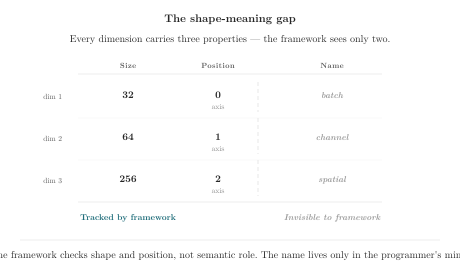
\includegraphics{figures/shape_meanings_gap.pdf}
\caption{Three properties of a coordinate: domain and position are
checked; the name is not}
\end{figure}

This is the shape-meanings gap. The shape says \emph{how many}. The role
says \emph{which one}. Every framework knows the shape. None of them
know the role.

\begin{center}\rule{0.5\linewidth}{0.4pt}\end{center}

Let's make this concrete. Here is a reduction:

\begin{Shaded}
\begin{Highlighting}[]
\NormalTok{x }\OperatorTok{=}\NormalTok{ torch.randn(}\DecValTok{32}\NormalTok{, }\DecValTok{64}\NormalTok{, }\DecValTok{256}\NormalTok{)}
\NormalTok{y }\OperatorTok{=}\NormalTok{ x.mean(dim}\OperatorTok{=}\DecValTok{1}\NormalTok{)}
\end{Highlighting}
\end{Shaded}

What was eliminated? The code says \texttt{dim=1}. If you are the
author, and you just wrote this line, you know that position 1 is
\texttt{channel}. If you are a colleague reading this six months later,
you have to reconstruct that fact. You look at the variable name. You
look for a comment. You trace the data pipeline backward. You hold your
breath and assume.

Now imagine a different notation:

\begin{Shaded}
\begin{Highlighting}[]
\KeywordTok{let}\NormalTok{ y}\OperatorTok{[}\NormalTok{b, s}\OperatorTok{]}\NormalTok{ = mean}\OperatorTok{[}\NormalTok{channel}\OperatorTok{]}\NormalTok{(x}\OperatorTok{[}\NormalTok{b, channel, s}\OperatorTok{]}\NormalTok{);}
\end{Highlighting}
\end{Shaded}

The bracket after \texttt{mean} names the coordinate being eliminated.
The brackets after \texttt{y} and \texttt{x} name the coordinates that
survive. The compiler checks that \texttt{channel} actually exists on
\texttt{x}. The reader sees the elimination without reconstructing it.
The fact that was previously in a comment---``average over
channels''---is now in the syntax, where the compiler can enforce it and
the reader can audit it.

This is not a hypothetical language. It is the one we will use for the
rest of this book. Its syntax first appears in Chapter 3. But the idea
it embodies---\textbf{give every dimension a name}---is independent of
any particular notation. You can practice it in NumPy docstrings, in
einops patterns, in the type annotations of your own code. The habit is
the payload. The syntax is only the delivery mechanism.

\begin{center}\rule{0.5\linewidth}{0.4pt}\end{center}

Before we move on, let's be precise about what ``naming a coordinate''
means.

A coordinate has three properties. First, a \textbf{name}:
\texttt{batch}, \texttt{channel}, \texttt{time}, \texttt{feature}. The
name carries the semantic role. Second, a \textbf{domain}: the set of
values the coordinate can take. For a tensor of shape
\texttt{(32,\ 64,\ 256)}, the \texttt{batch} coordinate ranges from
\texttt{0} to \texttt{31}, \texttt{channel} from \texttt{0} to
\texttt{63}, and \texttt{spatial} from \texttt{0} to \texttt{255}.
Third, a \textbf{position}: where this coordinate sits in the tensor's
shape tuple. In \texttt{(32,\ 64,\ 256)}, \texttt{batch} is at position
0, \texttt{channel} at position 1, \texttt{spatial} at position 2.

Positional notation records only the domain and the
position---\texttt{(32,\ 64,\ 256)} tells you the sizes and their order,
but not their names. Named notation records all three:
\texttt{{[}batch:\ 32,\ channel:\ 64,\ spatial:\ 256{]}}.

When you write \texttt{x.mean(dim=1)}, you are asking the position to
stand in for the name. It works until the position changes. When you
write \texttt{mean{[}channel{]}(x)}, you are using the name directly.
The position becomes an implementation detail---the compiler's problem,
not yours.

\begin{center}\rule{0.5\linewidth}{0.4pt}\end{center}

\hypertarget{an-analogy-the-parking-lot}{%
\subsection{An Analogy: The Parking
Lot}\label{an-analogy-the-parking-lot}}

You park your car in Row D, Slot 7. The ticket in your pocket says
``D-7.'' You return after dinner to find the lot has been repainted. The
rows now run perpendicular to their old orientation. Row D is now
somewhere else entirely. Your ticket, which records a \emph{position} in
a fixed coordinate system, sends you to the wrong car.

The lot's \emph{shape} hasn't changed. It is still an 8 × 20 grid. A
shape checker would tell you everything is fine. But the \emph{role} of
each row---which row is ``D''---has moved.

This is what happens when you write \texttt{x.transpose(1,\ 2)}. The
shape is still \texttt{(32,\ 256,\ 64)}. A shape checker sees the same
three numbers. But the positions have been reassigned. Dimension 1 is no
longer \texttt{channel}. Dimension 2 is no longer \texttt{spatial}. The
ticket in your pocket---\texttt{dim=1}---now points to the wrong car.

A named-coordinate notation is like a ticket that says ``the blue Honda
Civic'' instead of ``D-7.'' The car may move, but the description finds
it.

\begin{center}\rule{0.5\linewidth}{0.4pt}\end{center}

This chapter has said nothing you couldn't have figured out from fifteen
minutes with a debugger and a whiteboard. That is by design. The ideas
in Part I are simple. Their simplicity is the point.

The next chapter applies the same name-over-position instinct to a
second primitive: permutation.

\hypertarget{try-it}{%
\subsubsection{Try It}\label{try-it}}

\begin{enumerate}
\def\labelenumi{\arabic{enumi}.}
\item
  Open a Python REPL. Create \texttt{x\ =\ torch.randn(2,\ 3,\ 4)}.
  Decide which dimension is \texttt{batch}, which is \texttt{time},
  which is \texttt{feature}. Write that down on paper. Now write
  \texttt{x.mean(dim=1)}. Which dimension did you eliminate? If someone
  swapped dimensions 1 and 2 upstream, would your \texttt{mean} call
  still eliminate the one you intended?
\item
  The same exercise, but with \texttt{x.permute(0,\ 2,\ 1)}. Write down
  what the permutation \emph{means} in terms of your chosen coordinate
  names. Now imagine dimension 0 and dimension 1 are swapped upstream.
  Does your \texttt{permute(0,\ 2,\ 1)} still mean the same thing?
\end{enumerate}

\newpage

\hypertarget{chapter-2-moving-flowers-without-losing-the-trail}{%
\section{Chapter 2 · Moving Flowers Without Losing the
Trail}\label{chapter-2-moving-flowers-without-losing-the-trail}}

\begin{quote}
``The map is not the territory.''

--- Alfred Korzybski
\end{quote}

\emph{Primitives · Coordinate permutation}

\begin{center}\rule{0.5\linewidth}{0.4pt}\end{center}

A permutation is an operation that changes the order of dimensions
without changing any values. It is the simplest tensor operation there
is---no arithmetic, no reduction, just relabeling positions.

It is also a reliable source of 11 PM debugging sessions.

The problem is not that permutation is hard. The problem is that
positional permutation is a description of \emph{mechanics} rather than
\emph{intent}. The mechanics are correct. The intent is invisible. When
upstream changes the mechanics---same operation, different
positions---the intent silently drifts.

Here is a concrete example. An image-processing pipeline takes input in
\texttt{(batch,\ height,\ width,\ channel)} and needs it in
\texttt{(batch,\ channel,\ height,\ width)}:

\begin{Shaded}
\begin{Highlighting}[]
\NormalTok{x }\OperatorTok{=}\NormalTok{ x.permute(}\DecValTok{0}\NormalTok{, }\DecValTok{3}\NormalTok{, }\DecValTok{1}\NormalTok{, }\DecValTok{2}\NormalTok{)}
\end{Highlighting}
\end{Shaded}

The programmer writes this while looking at a diagram that says
``channel moves from position 3 to position 1.'' The diagram is correct.
The code is correct. Six months later, upstream changes its output
convention to \texttt{(batch,\ width,\ height,\ channel)}. Height and
width have swapped. \texttt{permute(0,\ 3,\ 1,\ 2)} still executes
without complaint. Channel still ends up at position 1---correct. But
height and width are now in positions the programmer did not intend. The
shapes are identical. The values are wrong.

No shape checker catches this. No type checker catches this. The bug
will surface in production as ``the model is slightly worse on images
with non-square aspect ratios,'' and it will take a human being several
hours to trace the silent swap back to this one line.

The root cause: \texttt{(0,\ 3,\ 1,\ 2)} describes a rearrangement of
\emph{positions}. What the programmer needed to describe was a
rearrangement of \emph{identities}---``move the dimension called
\texttt{channel} to the front, and keep everything else in order.''

\begin{center}\rule{0.5\linewidth}{0.4pt}\end{center}

\hypertarget{an-analogy-driving-directions}{%
\subsection{An Analogy: Driving
Directions}\label{an-analogy-driving-directions}}

Two sets of driving directions get you from the library to the bakery.

Set A: ``Turn left at the third light. Turn right at the second stop
sign. It's the fourth building on the right.''

Set B: ``Turn left from Main Street onto Oak Avenue. Turn right from Oak
onto Elm. It's the building between the post office and the park.''

Set A is positional. It works until a road closes, a light is removed,
or the city renumbers the blocks. Then ``the third light'' is a
different intersection. Set B is named. It works regardless of how the
roads are numbered, because it references identities that are stable
under infrastructure changes.

\begin{figure}
\centering
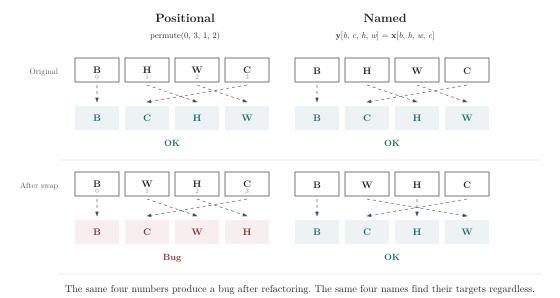
\includegraphics{figures/permute_survival.pdf}
\caption{Positional permute silently breaks when upstream changes; named
permute survives}
\end{figure}

The figure tests both notations against a common refactoring. Top row:
the original pipeline maps BHWC to BCHW. On the left,
\texttt{permute(0,3,1,2)}---read ``old axis 0 stays at 0, old axis 3
moves to 1, old axis 1 moves to 2, old axis 2 moves to 3''---produces
the correct result. Marked OK. On the right, the named expression
\texttt{y{[}b,c,h,w{]}\ =\ x{[}b,h,w,c{]}} produces the same correct
result. Both pass. Bottom row: upstream swaps height and width, so the
input is now BWHC. The positional instruction executes
identically---\texttt{permute(0,3,1,2)} is still the same four
numbers---but the output is now B,C,W,H. Height and width are silently
exchanged. Marked Bug. The named expression
\texttt{y{[}b,c,h,w{]}\ =\ x{[}b,h,w,c{]}} adapts automatically:
\texttt{h} maps to the second axis in the input regardless of where
height landed, \texttt{w} maps to the third. Marked OK. The instruction
did not change. The meaning did.

\texttt{permute(0,\ 3,\ 1,\ 2)} is Set A. It says ``take the dimension
at old position 0 and put it at new position 0, take old position 3 to
new position 1\ldots{}'' When upstream changes the dimension order, the
positions shift, and the same permute arguments produce a different
semantic result.

\texttt{y{[}b,\ c,\ h,\ w{]}\ =\ x{[}b,\ h,\ w,\ c{]}} is Set B. It says
``put the coordinate named \texttt{c} at position 1, regardless of where
it was before.'' When upstream changes, the coordinate name finds its
target.

The difference is not syntax. It is durability.

Einops addresses this with a string-based notation:

\begin{Shaded}
\begin{Highlighting}[]
\NormalTok{y }\OperatorTok{=}\NormalTok{ rearrange(x, }\StringTok{"batch height width channel -> batch channel height width"}\NormalTok{)}
\end{Highlighting}
\end{Shaded}

This is better. The names survive renaming of upstream positions,
because \texttt{rearrange} matches by name, not by index. A reader can
see what moved without reconstructing the position map.

But the string is still a string. The names \texttt{height} and
\texttt{width} are not checked against any declaration. They are local
to this one call. If the tensor actually contains \texttt{time} rather
than \texttt{height}, the string won't catch it---it will happily treat
\texttt{time} as if it were \texttt{height}, because the names in the
string are just pattern variables, not coordinate declarations.

What we want is for the coordinate names to be \textbf{checked facts},
not comments embedded in syntax:

\begin{Shaded}
\begin{Highlighting}[]
\KeywordTok{let}\NormalTok{ y}\OperatorTok{[}\NormalTok{b, c, h, w}\OperatorTok{]}\NormalTok{ = x}\OperatorTok{[}\NormalTok{b, h, w, c}\OperatorTok{]}\NormalTok{;}
\end{Highlighting}
\end{Shaded}

This is an einlang rectangular declaration. The left-hand side declares
the output coordinates. The right-hand side indexes the input by those
same coordinate names. \texttt{b} appears on both sides in the same
position---it survives unchanged. \texttt{h} appears on the left at
position 2 and on the right at position 1---it has been moved. The
compiler checks that every coordinate on the right actually exists on
\texttt{x}, and that every coordinate on the left appears somewhere on
the right.

You don't need a \texttt{permute} function. You don't need a
\texttt{rearrange} string. You just write where each coordinate goes,
and the compiler figures out the movement. The code says \emph{what you
want}, not \emph{how to achieve it}.

This is our first encounter with a pattern that will recur through the
entire book: \textbf{when coordinate names appear in the syntax,
operations become self-documenting.} The same line of code that
instructs the compiler also informs the reader. There is no separate
channel of documentation that can drift out of sync.

\begin{center}\rule{0.5\linewidth}{0.4pt}\end{center}

Positional permutation is not evil. It is the right abstraction for a
compiler pass that only needs to know ``move this stride to that
position.'' But source code is not written for compilers. It is written
for the human who will debug it at 11 PM, three months after the
original author left the team. That human needs to know \emph{what moved
where and why}. Position numbers answer the first question, but not the
second. Names answer both.

In the next chapter, we introduce a more dramatic operation: reduction.
A reduction does not merely rearrange coordinates. It eliminates one.
And the name of the eliminated coordinate matters more than any other.

\hypertarget{try-it-1}{%
\subsubsection{Try It}\label{try-it-1}}

\begin{enumerate}
\def\labelenumi{\arabic{enumi}.}
\item
  Take the permute bug from this chapter. Write down a convention for
  your own code that would have prevented it. Does your convention rely
  on variable names? Comments? Assertions? What happens to each of those
  when someone refactors the pipeline six months later?
\item
  In einops, write
  \texttt{rearrange(x,\ "batch\ time\ feature\ -\textgreater{}\ batch\ feature\ time")}.
  Now imagine \texttt{x} arrives with shape
  \texttt{(batch,\ feature,\ time)} instead. Does the rearrange still
  produce the correct result? Why or why not?
\end{enumerate}

\newpage

\hypertarget{chapter-3-a-small-farewell}{%
\section{Chapter 3 · A Small
Farewell}\label{chapter-3-a-small-farewell}}

\begin{quote}
``By relieving the brain of all unnecessary work, a good notation sets
it free to concentrate on more advanced problems.''

--- Alfred North Whitehead
\end{quote}

\emph{Primitives · Coordinate elimination and reduction}

\begin{center}\rule{0.5\linewidth}{0.4pt}\end{center}

A permutation moves coordinates around. A reduction makes one disappear.

This is a bigger deal than it sounds. When you eliminate a coordinate,
you are making an irreversible decision. All the variation along that
coordinate collapses into a single number. If you eliminate the wrong
coordinate, every downstream result is contaminated---not with a crash,
but with a mathematically valid answer to the wrong question.

And yet, in positional notation, a reduction is almost invisible.
\texttt{x.mean(dim=1)} is eight characters. The identity of the
eliminated coordinate occupies one of those characters: \texttt{1}. The
other seven are ceremony.

This chapter introduces the first einlang syntax. We're going to write
tensor operations where the eliminated coordinate is named
explicitly---where the code says \emph{what was lost}, not just
\emph{where it used to live}.

\begin{center}\rule{0.5\linewidth}{0.4pt}\end{center}

\hypertarget{rectangular-declarations}{%
\subsection{Rectangular Declarations}\label{rectangular-declarations}}

Before we can eliminate a coordinate, we need to name the ones we're
keeping. In einlang, you name coordinates with a \textbf{rectangular
declaration}:

\begin{Shaded}
\begin{Highlighting}[]
\KeywordTok{let}\NormalTok{ doubled}\OperatorTok{[}\NormalTok{i, j}\OperatorTok{]}\NormalTok{ = matrix}\OperatorTok{[}\NormalTok{i, j}\OperatorTok{]}\NormalTok{ * }\DecValTok{2.0}\NormalTok{;}
\end{Highlighting}
\end{Shaded}

Let's read this carefully. The \texttt{let} binds a new, immutable
tensor. The \texttt{{[}i,\ j{]}} on the left declares the output
coordinates---the new tensor will have two dimensions, and we are naming
them \texttt{i} and \texttt{j}. The \texttt{matrix{[}i,\ j{]}} on the
right indexes the input tensor \texttt{matrix} by those same
coordinates. The compiler infers that \texttt{i} ranges from \texttt{0}
to \texttt{matrix.shape{[}0{]}} and \texttt{j} from \texttt{0} to
\texttt{matrix.shape{[}1{]}}.

This is not a loop. It is a declaration. You are stating a fact: ``for
all \texttt{i} and \texttt{j} in their respective domains,
\texttt{doubled{[}i,\ j{]}} equals \texttt{matrix{[}i,\ j{]}\ *\ 2.0}.''
The compiler handles the iteration. You handle the meaning.

The index slots in the declaration bracket can take four forms:

\begin{itemize}
\tightlist
\item
  \textbf{A name}: \texttt{i}, \texttt{j}, \texttt{batch},
  \texttt{channel}---the standard case. The compiler infers the range
  from how the name is used in the body.
\item
  \textbf{A name with an explicit domain}: \texttt{i\ in\ 0..n}---when
  you need to control the range directly.
\item
  \textbf{A literal}: \texttt{0}---used for base cases in recurrences
  (we'll see these in Chapter 9).
\item
  \textbf{A named rest}: \texttt{..batch}---stands for zero or more
  adjacent axes. We'll meet these in the next chapter.
\end{itemize}

\begin{center}\rule{0.5\linewidth}{0.4pt}\end{center}

\hypertarget{reduction}{%
\subsection{Reduction}\label{reduction}}

Now the main event. A reduction iterates over a coordinate and combines
all the values along it using an associative operation. The coordinate
appears in the reduction bracket---and then it is gone from the result:

\begin{Shaded}
\begin{Highlighting}[]
\KeywordTok{let}\NormalTok{ total = sum}\OperatorTok{[}\NormalTok{i}\OperatorTok{]}\NormalTok{(data}\OperatorTok{[}\NormalTok{i}\OperatorTok{]}\NormalTok{);}
\end{Highlighting}
\end{Shaded}

\texttt{sum{[}i{]}(...)} says: for every value of \texttt{i}, evaluate
the body \texttt{data{[}i{]}}, and sum the results. The coordinate
\texttt{i} is introduced by the \texttt{sum}, used in the body, and
consumed by the reduction. It does not appear in
\texttt{total}---\texttt{total} is a scalar.

The four reduction operations are \texttt{sum}, \texttt{max},
\texttt{min}, and \texttt{prod}. Each has an identity element that fills
in when the domain is empty: \texttt{sum} starts from \texttt{0},
\texttt{prod} from \texttt{1}, \texttt{max} from negative infinity,
\texttt{min} from positive infinity.

A reduction can eliminate multiple coordinates at once:

\begin{Shaded}
\begin{Highlighting}[]
\KeywordTok{let}\NormalTok{ grand_total = sum}\OperatorTok{[}\NormalTok{i, j}\OperatorTok{]}\NormalTok{(matrix}\OperatorTok{[}\NormalTok{i, j}\OperatorTok{]}\NormalTok{);}
\end{Highlighting}
\end{Shaded}

And a reduction can leave some coordinates intact---producing a tensor
rather than a scalar:

\begin{Shaded}
\begin{Highlighting}[]
\KeywordTok{let}\NormalTok{ row_sums}\OperatorTok{[}\NormalTok{i}\OperatorTok{]}\NormalTok{ = sum}\OperatorTok{[}\NormalTok{j}\OperatorTok{]}\NormalTok{(matrix}\OperatorTok{[}\NormalTok{i, j}\OperatorTok{]}\NormalTok{);}
\KeywordTok{let}\NormalTok{ col_sums}\OperatorTok{[}\NormalTok{j}\OperatorTok{]}\NormalTok{ = sum}\OperatorTok{[}\NormalTok{i}\OperatorTok{]}\NormalTok{(matrix}\OperatorTok{[}\NormalTok{i, j}\OperatorTok{]}\NormalTok{);}
\end{Highlighting}
\end{Shaded}

These two lines produce the same output shape (a 1D tensor of length
equal to the surviving coordinate). But they mean completely different
things. \texttt{row\_sums{[}i{]}} sums over columns, leaving rows.
\texttt{col\_sums{[}j{]}} sums over rows, leaving columns. The
difference is entirely in the bracket after \texttt{sum}---one
character, carrying the full semantic weight of the operation.

In a positional API, these would be \texttt{matrix.sum(dim=1)} and
\texttt{matrix.sum(dim=0)}. The reader must remember which position is
rows and which is columns. The code does not help.

\begin{center}\rule{0.5\linewidth}{0.4pt}\end{center}

\hypertarget{matrix-multiplication}{%
\subsection{Matrix Multiplication}\label{matrix-multiplication}}

With rectangular declarations and reductions, we have enough machinery
to write matrix multiplication:

\begin{Shaded}
\begin{Highlighting}[]
\KeywordTok{let}\NormalTok{ C}\OperatorTok{[}\NormalTok{i, j}\OperatorTok{]}\NormalTok{ = sum}\OperatorTok{[}\NormalTok{k}\OperatorTok{]}\NormalTok{(A}\OperatorTok{[}\NormalTok{i, k}\OperatorTok{]}\NormalTok{ * B}\OperatorTok{[}\NormalTok{k, j}\OperatorTok{]}\NormalTok{);}
\end{Highlighting}
\end{Shaded}

\begin{figure}
\centering
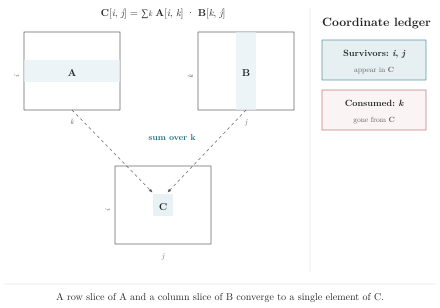
\includegraphics{figures/matmul_coords.pdf}
\caption{Coordinates flow through matmul: i and j survive, k is
consumed}
\end{figure}

The figure lays out the three matrices. \(\mathbf{A}\) carries
coordinates \(\{i, k\}\)---rows indexed by \(i\), columns by \(k\).
\(\mathbf{B}\) carries \(\{k, j\}\)---rows indexed by \(k\), columns by
\(j\). The \texttt{sum{[}k{]}} bracket between them names the coordinate
they share and that the reduction consumes. \(\mathbf{C}\) carries
\(\{i, j\}\)---only the survivors. On the right, a two-column ledger
partitions the coordinates: \(i\) and \(j\) in the Survivors column
(they appear in \(\mathbf{C}\)), \(k\) in the Consumed column (gone from
\(\mathbf{C}\)). This ledger is the visual form of the coordinate-audit
instinct we are building.

If you've taken a linear algebra course, this line needs no explanation.
It is the mathematical definition of matrix multiplication, transcribed
character for character:

\[C_{ij} = \sum_k A_{ik} B_{kj}\]

The coordinate \texttt{k} is introduced by \texttt{sum}, used to index
both \texttt{A} and \texttt{B} (forcing their shared dimension to
agree---the compiler checks this), and consumed. The coordinates
\texttt{i} and \texttt{j} survive into the result.

Notice what this line does \emph{not} contain: - No \texttt{transpose}.
The indexing pattern \texttt{B{[}k,\ j{]}} naturally expresses that
\texttt{B}'s rows are \texttt{k} and columns are \texttt{j}. - No
\texttt{matmul} function name. The operation is defined by the
coordinates. - No \texttt{@} operator whose meaning you have to look up.

The line says exactly what it means. And if you get the coordinates
wrong---if you write \texttt{B{[}j,\ k{]}} instead of
\texttt{B{[}k,\ j{]}}---the compiler catches it, because \texttt{k}'s
range from \texttt{A} won't match \texttt{j}'s range from \texttt{B}.

\begin{center}\rule{0.5\linewidth}{0.4pt}\end{center}

\hypertarget{how-to-read-a-reduction-the-two-column-ledger}{%
\subsection{How to Read a Reduction: The Two-Column
Ledger}\label{how-to-read-a-reduction-the-two-column-ledger}}

A reduction is the most semantically loaded operation in tensor
programming. Every reduction is making two claims at once: which
coordinate is being \emph{consumed} (gone from the result), and which
coordinates are \emph{surviving} (present in the result). When you read
a reduction, draw an imaginary line down the middle of the page:

\begin{longtable}[]{@{}ll@{}}
\toprule
\begin{minipage}[b]{0.54\columnwidth}\raggedright
Survivors\strut
\end{minipage} & \begin{minipage}[b]{0.40\columnwidth}\raggedright
Locals\strut
\end{minipage}\tabularnewline
\midrule
\endhead
\begin{minipage}[t]{0.54\columnwidth}\raggedright
Coordinates that appear in the result\strut
\end{minipage} & \begin{minipage}[t]{0.40\columnwidth}\raggedright
Coordinates introduced in the reduction bracket\strut
\end{minipage}\tabularnewline
\begin{minipage}[t]{0.54\columnwidth}\raggedright
They keep their identity across the operation\strut
\end{minipage} & \begin{minipage}[t]{0.40\columnwidth}\raggedright
They are consumed---gone from the output\strut
\end{minipage}\tabularnewline
\begin{minipage}[t]{0.54\columnwidth}\raggedright
They can be used by later operations\strut
\end{minipage} & \begin{minipage}[t]{0.40\columnwidth}\raggedright
They exist only within the reduction body\strut
\end{minipage}\tabularnewline
\bottomrule
\end{longtable}

For \texttt{let\ row\_sums{[}i{]}\ =\ sum{[}j{]}(matrix{[}i,\ j{]});}:

\begin{itemize}
\tightlist
\item
  \textbf{Survivors}: \texttt{i} (appears on the left-hand side,
  survives into \texttt{row\_sums})
\item
  \textbf{Locals}: \texttt{j} (introduced by \texttt{sum{[}j{]}},
  consumed, gone)
\end{itemize}

For
\texttt{let\ C{[}i,\ j{]}\ =\ sum{[}k{]}(A{[}i,\ k{]}\ *\ B{[}k,\ j{]});}:

\begin{itemize}
\tightlist
\item
  \textbf{Survivors}: \texttt{i}, \texttt{j} (appear on the left,
  survive into \texttt{C})
\item
  \textbf{Locals}: \texttt{k} (introduced by \texttt{sum{[}k{]}}, aligns
  \texttt{A} and \texttt{B}, consumed)
\end{itemize}

This ledger is the coordinate audit in miniature. Every reduction you
encounter, pause and fill in the two columns. If you can't fill them in
from the code alone---if you need to print shapes or consult a
comment---the code is hiding information that the notation should have
recorded.

A five-step rule for reading any reduction:

\begin{enumerate}
\def\labelenumi{\arabic{enumi}.}
\tightlist
\item
  \textbf{Identity the reduction}: which operation (\texttt{sum},
  \texttt{max}, \texttt{min}, \texttt{prod}) and which coordinates are
  in its bracket?
\item
  \textbf{Identify the survivors}: which coordinates appear on the
  left-hand side of the \texttt{let}?
\item
  \textbf{Identify the consumed}: which coordinates appear in the
  reduction bracket but not on the left?
\item
  \textbf{Verify alignment}: do the consumed coordinates index matching
  positions across all terms in the body?
\item
  \textbf{State the claim}: in one sentence, what does this reduction
  assert? ``For each \texttt{i}, sum over all \texttt{j}.'' ``For each
  \texttt{{[}b,\ out{]}}, contract \texttt{{[}in{]}} between the input
  and the weight.''
\end{enumerate}

This takes five seconds. It catches the bug where
\texttt{sum{[}class{]}} silently became \texttt{sum{[}batch{]}} after a
refactoring.

\begin{center}\rule{0.5\linewidth}{0.4pt}\end{center}

\hypertarget{what-weve-just-learned}{%
\subsection{What We've Just Learned}\label{what-weve-just-learned}}

This chapter introduced three things that will carry us through the rest
of the book:

\begin{enumerate}
\def\labelenumi{\arabic{enumi}.}
\tightlist
\item
  \textbf{Rectangular declarations} (\texttt{let\ C{[}i,\ j{]}\ =\ ...})
  name the coordinates of a new tensor and define its values by indexing
  existing tensors.
\item
  \textbf{Reductions} (\texttt{sum{[}k{]}(...)},
  \texttt{max{[}k{]}(...)}, \texttt{min{[}k{]}(...)},
  \texttt{prod{[}k{]}(...)}) consume a coordinate---they introduce it in
  the reduction bracket, use it in the body, and erase it from the
  result.
\item
  \textbf{Coordinates are checked, not commented.} When you write
  \texttt{sum{[}k{]}(A{[}i,\ k{]}\ *\ B{[}k,\ j{]})}, the compiler
  verifies that \texttt{A} has a \texttt{k} dimension, that \texttt{B}
  has a \texttt{k} dimension, and that their ranges agree. A typo in a
  coordinate name is a compile error, not a runtime mystery.
\end{enumerate}

We are still in the primitives layer. We've learned to name coordinates
and to eliminate them. In the next chapter, we learn the third
primitive: when a coordinate is \emph{copied} rather than eliminated.

\hypertarget{try-it-2}{%
\subsubsection{Try It}\label{try-it-2}}

\begin{enumerate}
\def\labelenumi{\arabic{enumi}.}
\item
  Write the einlang expression for a vector dot product: given two 1D
  tensors \texttt{a{[}i{]}} and \texttt{b{[}i{]}}, produce a scalar
  \texttt{dot}. Compare it to \texttt{torch.dot(a,\ b)}. Which version
  tells you which coordinate was summed?
\item
  Write the einlang expression for
  \texttt{torch.nn.functional.linear(input,\ weight,\ bias)}---a linear
  layer that computes
  \texttt{output{[}b,\ out{]}\ =\ sum{[}in{]}(input{[}b,\ in{]}\ *\ weight{[}out,\ in{]})\ +\ bias{[}out{]}}.
  Identify which coordinates survive, which is consumed, and which is
  omitted from the bias term.
\item
  A friend writes
  \texttt{let\ C{[}i,\ j{]}\ =\ sum{[}k{]}(A{[}i,\ k{]}\ *\ B{[}j,\ k{]});}
  thinking it's matrix multiplication. Is it? If not, what is it
  computing, and why does the compiler accept it?
\end{enumerate}

\newpage

\hypertarget{chapter-4-copy-and-a-promise}{%
\section{Chapter 4 · Copy, and a
Promise}\label{chapter-4-copy-and-a-promise}}

\begin{quote}
``The absence of a signal is itself a signal.''

--- Geoffrey Hinton (apocryphal)
\end{quote}

\emph{Primitives · Broadcasting}

\begin{center}\rule{0.5\linewidth}{0.4pt}\end{center}

Broadcasting is one of the most convenient features of modern tensor
frameworks. It lets you write \texttt{x\ +\ bias} when \texttt{x} has
shape \texttt{(32,\ 64)} and \texttt{bias} has shape
\texttt{(64,)}---the framework silently expands \texttt{bias} along the
missing dimension, as if you'd written
\texttt{x\ +\ bias.repeat(32,\ 1)}. It saves keystrokes. It saves
memory. It reads cleanly.

It also buries a semantic claim inside a shape-compatibility rule.

The shape rule says: if a dimension has size 1 in one operand, it can be
expanded to match the other operand's size at that position. The
semantic claim says: the value along that dimension is \emph{truly
independent} of the coordinate being expanded. If \texttt{bias} has
shape \texttt{(64,)} and you add it to \texttt{x} of shape
\texttt{(32,\ 64)}, you are asserting that \texttt{bias} does not depend
on \texttt{batch}---that the same 64 values apply identically to every
one of the 32 batch elements.

The shape rule is checked by the compiler. The semantic claim is checked
by no one.

When the claim is true, broadcasting is a clean, memory-efficient
notation for a genuine structural fact. When the claim is false---when
\texttt{bias} actually \emph{does} vary with batch, but you accidentally
loaded it at the wrong shape---broadcasting silently smears the wrong
values across 32 batch elements. The shapes are compatible. The result
is wrong.

\begin{center}\rule{0.5\linewidth}{0.4pt}\end{center}

\hypertarget{broadcasting-in-einlang}{%
\subsection{Broadcasting in einlang}\label{broadcasting-in-einlang}}

Einlang takes a deliberate position: broadcasting is allowed, but only
in cases where no coordinate name needs to be inferred. There are
exactly two cases:

\textbf{Same-rank broadcasting.} Two tensors with identical shapes can
be combined elementwise. No expansion needed:

\begin{Shaded}
\begin{Highlighting}[]
\KeywordTok{let}\NormalTok{ sum_AB}\OperatorTok{[}\NormalTok{i, j}\OperatorTok{]}\NormalTok{ = A}\OperatorTok{[}\NormalTok{i, j}\OperatorTok{]}\NormalTok{ + B}\OperatorTok{[}\NormalTok{i, j}\OperatorTok{]}\NormalTok{;}
\end{Highlighting}
\end{Shaded}

\textbf{Scalar broadcasting.} A scalar can be combined with any tensor:

\begin{Shaded}
\begin{Highlighting}[]
\KeywordTok{let}\NormalTok{ scaled}\OperatorTok{[}\NormalTok{i, j}\OperatorTok{]}\NormalTok{ = matrix}\OperatorTok{[}\NormalTok{i, j}\OperatorTok{]}\NormalTok{ * }\DecValTok{2.0}\NormalTok{;}
\KeywordTok{let}\NormalTok{ shifted}\OperatorTok{[}\NormalTok{i, j}\OperatorTok{]}\NormalTok{ = matrix}\OperatorTok{[}\NormalTok{i, j}\OperatorTok{]}\NormalTok{ + }\DecValTok{10.0}\NormalTok{;}
\end{Highlighting}
\end{Shaded}

The scalar case is unambiguous---there are no coordinate names to infer,
because a scalar has no coordinates.

\textbf{Everything else requires explicit indexing.} If you want to add
a vector bias to a matrix, you must write the coordinate that the bias
omits:

\begin{figure}
\centering
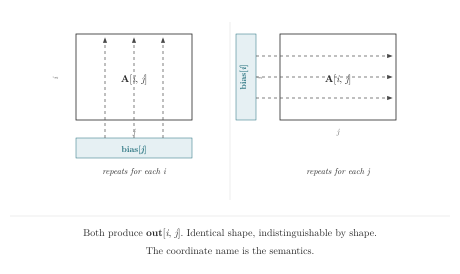
\includegraphics{figures/broadcasting.pdf}
\caption{Feature bias vs batch bias: same shape, two meanings}
\end{figure}

\begin{Shaded}
\begin{Highlighting}[]
\KeywordTok{let}\NormalTok{ out}\OperatorTok{[}\NormalTok{i, j}\OperatorTok{]}\NormalTok{ = A}\OperatorTok{[}\NormalTok{i, j}\OperatorTok{]}\NormalTok{ + bias}\OperatorTok{[}\NormalTok{j}\OperatorTok{]}\NormalTok{;}
\end{Highlighting}
\end{Shaded}

The coordinate \texttt{i} appears on \texttt{A} and \texttt{out}, but
not on \texttt{bias}. Its absence from \texttt{bias} is the notation for
broadcasting: \texttt{bias} is indexed only by \texttt{j}, so it is
replicated across all values of \texttt{i}. The code states the semantic
claim directly---\texttt{bias} does not depend on \texttt{i}---and the
claim is visible to both the reader and the compiler.

Compare this to the implicit version: \texttt{A\ +\ bias}. The shapes
match. The broadcast happens. But \emph{which coordinate was broadcast
over}? You have to know the shapes to answer that. And if the shapes
change upstream, the answer changes with them, silently.

\begin{center}\rule{0.5\linewidth}{0.4pt}\end{center}

\hypertarget{named-rest-..batch}{%
\subsection{\texorpdfstring{Named Rest:
\texttt{..batch}}{Named Rest: ..batch}}\label{named-rest-..batch}}

So far our coordinates have been single, explicit names. But real tensor
code often needs to be polymorphic over how many batch dimensions there
are. A normalization function shouldn't care whether the input is
\texttt{(batch,\ feature)}, \texttt{(batch,\ time,\ feature)}, or
\texttt{(batch,\ head,\ time,\ feature)}. It only cares that
\texttt{feature} is the last dimension and everything else is
batch-like.

Einlang provides \textbf{named rest indices} for this:

\begin{Shaded}
\begin{Highlighting}[]
\KeywordTok{let}\NormalTok{ result}\OperatorTok{[}\NormalTok{..batch, j}\OperatorTok{]}\NormalTok{ = x}\OperatorTok{[}\NormalTok{..batch, j}\OperatorTok{]}\NormalTok{ + bias}\OperatorTok{[}\NormalTok{j}\OperatorTok{]}\NormalTok{;}
\KeywordTok{let}\NormalTok{ row_sum}\OperatorTok{[}\NormalTok{..batch}\OperatorTok{]}\NormalTok{ = sum}\OperatorTok{[}\NormalTok{j}\OperatorTok{]}\NormalTok{(x}\OperatorTok{[}\NormalTok{..batch, j}\OperatorTok{]}\NormalTok{);}
\end{Highlighting}
\end{Shaded}

The notation \texttt{..batch} stands for zero or more adjacent axes,
collectively referred to as \texttt{batch}. The same rest name must
describe the same axis span everywhere it appears within an expression.
The compiler infers which concrete axes \texttt{..batch} covers from the
shape of \texttt{x}.

This is not a wildcard. It is a named group. The name \texttt{batch}
carries semantic weight---it says ``these leading dimensions are all
batch-like, and the operation treats them uniformly.'' If upstream adds
a \texttt{head} dimension between \texttt{batch} and \texttt{time},
\texttt{..batch} absorbs it automatically. If upstream removes a
dimension, \texttt{..batch} shrinks. The code does not need to change,
because the code was written in terms of \emph{roles}, not positions.

\begin{center}\rule{0.5\linewidth}{0.4pt}\end{center}

\hypertarget{the-principle-of-explicit-omission}{%
\subsection{The Principle of Explicit
Omission}\label{the-principle-of-explicit-omission}}

Broadcasting is not the only way a coordinate can be absent from an
expression. Any time a coordinate appears in the output but not in a
particular input term, that term is being implicitly replicated along
that coordinate. The pattern is:

\begin{Shaded}
\begin{Highlighting}[]
\KeywordTok{let}\NormalTok{ y}\OperatorTok{[}\NormalTok{i, j, k}\OperatorTok{]}\NormalTok{ = term1}\OperatorTok{[}\NormalTok{i, j}\OperatorTok{]}\NormalTok{ + term2}\OperatorTok{[}\NormalTok{j, k}\OperatorTok{]}\NormalTok{;}
\end{Highlighting}
\end{Shaded}

\texttt{term1} omits \texttt{k}---it is replicated along \texttt{k}.
\texttt{term2} omits \texttt{i}---it is replicated along \texttt{i}.
Both omissions are visible in the indexing pattern, because the
coordinates are written explicitly.

This is the principle of explicit omission: \textbf{if a term is
independent of a coordinate, the indexing should show it.} When the
indexing shows it, the reader can audit it. When the indexing hides it,
the reader must guess.

In the next chapter, we'll see what happens when broadcasting promises
interact with gradients. A forward broadcast is a promise of
independence. A backward gradient collects dependence. The two
directions must agree---and when they don't, the bug is invisible to
shape checks but visible to named coordinates.

\textbf{The Inversion Rule.} Broadcast and reduction are inverses. What
you broadcast over in the forward pass, you reduce over in the backward
pass. \texttt{bias{[}j{]}} omits \texttt{i} in the forward
direction---broadcast.
\texttt{dbias{[}j{]}\ =\ sum{[}i{]}(dy{[}i,\ j{]})} consumes \texttt{i}
in the backward direction---reduction. The omitted coordinate and the
consumed coordinate are the same coordinate. Memorize this pairing. It
catches more bugs than any other single rule in this book.

\hypertarget{try-it-3}{%
\subsubsection{Try It}\label{try-it-3}}

\begin{enumerate}
\def\labelenumi{\arabic{enumi}.}
\item
  In PyTorch, write
  \texttt{x\ =\ torch.randn(8,\ 10);\ b\ =\ torch.randn(10);\ y\ =\ x\ +\ b}.
  What shape is \texttt{b} broadcast over? Now imagine \texttt{x} is
  transposed upstream to shape \texttt{(10,\ 8)}. Does \texttt{x\ +\ b}
  still work? What does it now broadcast over? Is that what you
  intended?
\item
  Write an einlang declaration that adds a per-class bias
  \texttt{class\_bias{[}c{]}} to a logit tensor
  \texttt{logits{[}b,\ c{]}}. Which coordinate is the bias independent
  of? How does the code make that independence visible?
\item
  What does
  \texttt{let\ out{[}..rest,\ c{]}\ =\ x{[}..rest,\ c{]}\ +\ shift{[}c{]};}
  do if \texttt{x} has shape \texttt{(2,\ 3,\ 4,\ 5)}? What if
  \texttt{x} has shape \texttt{(6,\ 7)}?
\end{enumerate}

\newpage

\hypertarget{chapter-5-when-promises-chain-together}{%
\section{Chapter 5 · When Promises Chain
Together}\label{chapter-5-when-promises-chain-together}}

\begin{quote}
``Trust, but verify.''

--- Russian proverb
\end{quote}

\emph{Primitives to Combinations · Broadcast self-audit, where clauses,
and the first look at gradients}

\begin{center}\rule{0.5\linewidth}{0.4pt}\end{center}

Chapter 4 ended with a principle: when a term omits a coordinate, it
promises independence from that coordinate. This chapter asks what
happens when those promises interact---when one operation's broadcast
feeds into another operation's reduction, when gradients flow backward
through a broadcast, and when a conditional guard depends on the very
values being combined.

We are crossing the bridge from primitives to combinations. The
operations are still elementary, but we are about to compose them in
ways that reveal hidden structure.

\begin{center}\rule{0.5\linewidth}{0.4pt}\end{center}

\hypertarget{the-broadcast-self-audit}{%
\subsection{The Broadcast Self-Audit}\label{the-broadcast-self-audit}}

A forward broadcast makes a promise. A backward gradient collects
dependence. If the two disagree, the gradient is silently wrong.

Consider a linear layer with a bias:

\begin{Shaded}
\begin{Highlighting}[]
\KeywordTok{let}\NormalTok{ z}\OperatorTok{[}\NormalTok{b, out}\OperatorTok{]}\NormalTok{ = sum}\OperatorTok{[}\KeywordTok{in}\OperatorTok{]}\NormalTok{(x}\OperatorTok{[}\NormalTok{b, }\KeywordTok{in}\OperatorTok{]}\NormalTok{ * W}\OperatorTok{[}\NormalTok{out, }\KeywordTok{in}\OperatorTok{]}\NormalTok{) + bias}\OperatorTok{[}\NormalTok{out}\OperatorTok{]}\NormalTok{;}
\end{Highlighting}
\end{Shaded}

The bias term omits \texttt{b}---it promises that the bias does not
depend on the batch element. The forward pass is correct. Now compute
the gradient of the loss with respect to the bias:

\begin{Shaded}
\begin{Highlighting}[]
\KeywordTok{let}\NormalTok{ d_bias}\OperatorTok{[}\NormalTok{out}\OperatorTok{]}\NormalTok{ = sum}\OperatorTok{[}\NormalTok{b}\OperatorTok{]}\NormalTok{(d_loss}\OperatorTok{[}\NormalTok{b, out}\OperatorTok{]}\NormalTok{);}
\end{Highlighting}
\end{Shaded}

The gradient sums over \texttt{b}. Why? Because in the forward pass,
\texttt{bias{[}out{]}} was replicated across every batch element. Every
batch element carries a piece of the gradient signal. To update
\texttt{bias}, we must collect all those pieces. The omitted coordinate
becomes the reduced coordinate in the backward pass.

This is the broadcast-reduce duality: \textbf{what you broadcast over in
the forward pass, you reduce over in the backward pass.}

Now ask yourself three questions about any broadcast in your code:

\begin{enumerate}
\def\labelenumi{\arabic{enumi}.}
\tightlist
\item
  \textbf{What coordinate am I broadcasting over?} Is the name visible
  in the code, or is it inferred from position?
\item
  \textbf{Is independence truly justified?} Does the broadcast value
  genuinely not depend on that coordinate, or is this a shape
  coincidence?
\item
  \textbf{What will the gradient do?} In the backward pass, the
  broadcast coordinate becomes a reduction coordinate. Does that
  reduction produce the right shape for the parameter update?
\end{enumerate}

These three questions are the broadcast self-audit. They cost nothing to
ask. They catch the class of bugs where a broadcast is shape-correct but
semantically wrong.

\begin{center}\rule{0.5\linewidth}{0.4pt}\end{center}

\hypertarget{introducing-y-x}{%
\subsection{\texorpdfstring{Introducing
\texttt{@y\ /\ @x}}{Introducing @y / @x}}\label{introducing-y-x}}

Einlang provides built-in automatic differentiation. You don't call
\texttt{loss.backward()}. You don't register hooks. You write the
derivative you want directly:

\begin{Shaded}
\begin{Highlighting}[]
\KeywordTok{let}\NormalTok{ x = }\DecValTok{1.0}\NormalTok{;}
\KeywordTok{let}\NormalTok{ y = }\DecValTok{2.0}\NormalTok{;}
\KeywordTok{let}\NormalTok{ z = x + y;}
\KeywordTok{let}\NormalTok{ dz_dx = @z / @x;   }\CommentTok{// 1.0}
\KeywordTok{let}\NormalTok{ dz_dy = @z / @y;   }\CommentTok{// 1.0}
\end{Highlighting}
\end{Shaded}

\texttt{@z\ /\ @x} is an expression, not a framework call. It means
``the derivative of the named binding \texttt{z} with respect to the
named binding \texttt{x}.'' For scalars, it evaluates to a number. The
compiler computes it through the chain rule, tracing the dependency
graph you constructed with \texttt{let} bindings.

We will explore automatic differentiation in depth in Chapter 8. For
now, we use it in the simplest possible way: as a tool for verifying
that our broadcast contracts are self-consistent. If the gradient has
the wrong shape, the broadcast was wrong. If the gradient sums over a
coordinate you didn't expect, your broadcast omitted a coordinate you
didn't intend.

\texttt{@z\ /\ @x} is a diagnostic instrument before it is an
optimization tool. Point it at any broadcast. The shape of the result
will tell you whether the broadcast contract holds.

\begin{center}\rule{0.5\linewidth}{0.4pt}\end{center}

\hypertarget{the-where-clause}{%
\subsection{\texorpdfstring{The \texttt{where}
Clause}{The where Clause}}\label{the-where-clause}}

Sometimes a computation should only apply to a subset of coordinate
values. In a positional API, you'd create a mask tensor, multiply, and
hope the mask doesn't silently broadcast into the wrong dimension. In
einlang, you attach a \textbf{\texttt{where} clause} directly to the
declaration:

\begin{Shaded}
\begin{Highlighting}[]
\KeywordTok{let}\NormalTok{ pos_sum = sum}\OperatorTok{[}\NormalTok{i}\OperatorTok{]}\NormalTok{(data}\OperatorTok{[}\NormalTok{i}\OperatorTok{]}\NormalTok{) }\KeywordTok{where}\NormalTok{ data}\OperatorTok{[}\NormalTok{i}\OperatorTok{]}\NormalTok{ > }\DecValTok{0}\NormalTok{;}
\end{Highlighting}
\end{Shaded}

The where clause is evaluated for each combination of the enclosing
index variables. For reductions, elements where the guard is false are
skipped---the reduction's identity element is used instead. For
rectangular declarations, filtered-out positions receive the default
value (zero for numeric types).

A where clause can also bind intermediate variables to avoid
recomputation:

\begin{Shaded}
\begin{Highlighting}[]
\KeywordTok{let}\NormalTok{ output}\OperatorTok{[}\NormalTok{i, j}\OperatorTok{]}\NormalTok{ = activated}
    \KeywordTok{where}\NormalTok{ z = sum}\OperatorTok{[}\NormalTok{k}\OperatorTok{]}\NormalTok{(input}\OperatorTok{[}\NormalTok{i, k}\OperatorTok{]}\NormalTok{ * weight}\OperatorTok{[}\NormalTok{k, j}\OperatorTok{]}\NormalTok{) + bias}\OperatorTok{[}\NormalTok{j}\OperatorTok{]}\NormalTok{,}
\NormalTok{          activated = }\KeywordTok{if}\NormalTok{ z > }\DecValTok{0.0} \OperatorTok{\{}\NormalTok{ z }\OperatorTok{\}} \KeywordTok{else} \OperatorTok{\{} \DecValTok{0.0} \OperatorTok{\}}\NormalTok{;}
\end{Highlighting}
\end{Shaded}

Without the where clause, you'd write the \texttt{sum{[}k{]}(...)}
expression twice---once for the comparison and once for the value. With
the where clause, you name the shared subexpression \texttt{z} and refer
to it in \texttt{activated}. The bindings are evaluated in order; later
bindings can reference earlier ones.

The where clause is not a separate language feature bolted onto tensor
operations. It is the natural extension of the idea that declarations
state facts over coordinate domains. A where clause narrows the domain
over which the fact holds. The syntax reflects the semantics directly.

\begin{center}\rule{0.5\linewidth}{0.4pt}\end{center}

\hypertarget{from-primitives-to-combinations}{%
\subsection{From Primitives to
Combinations}\label{from-primitives-to-combinations}}

We have now covered the four primitives of tensor computation: -
\textbf{Naming} (Chapter 1): every dimension gets a name tag. -
\textbf{Permutation} (Chapter 2): coordinate movement is stated in terms
of names, not positions. - \textbf{Reduction} (Chapter 3): a consumed
coordinate is named in the reduction bracket. - \textbf{Broadcasting}
(Chapter 4): an omitted coordinate is visible by its absence from an
index list.

We have also introduced our first means of combining these primitives:
the where clause (which scopes a computation over a restricted
coordinate domain) and the derivative operator (which reverses the flow
of dependence).

In the next chapter, we give the language a name and learn how to
combine primitives not just in single declarations, but in functions
that carry coordinate information across call boundaries.

\hypertarget{try-it-4}{%
\subsubsection{Try It}\label{try-it-4}}

\begin{enumerate}
\def\labelenumi{\arabic{enumi}.}
\item
  Given
  \texttt{let\ z{[}b,\ o{]}\ =\ sum{[}i{]}(x{[}b,\ i{]}\ *\ W{[}o,\ i{]})\ +\ bias{[}o{]};},
  write the gradient \texttt{@z\ /\ @bias}. What coordinate does it sum
  over? Why that one?
\item
  Write an einlang expression that sums only the positive elements of
  \texttt{data{[}i{]}}, divided by the count of positive elements (i.e.,
  the mean of positive values). Use a where clause. Compare the number
  of lines to the equivalent PyTorch.
\item
  A colleague writes
  \texttt{let\ y{[}b,\ f{]}\ =\ x{[}b,\ f{]}\ +\ scale{[}f{]}\ where\ scale{[}f{]}\ \textgreater{}\ 0;}.
  What does this do? Is it correct?
\end{enumerate}

\newpage

\hypertarget{chapter-6-putting-the-pieces-together}{%
\section{Chapter 6 · Putting the Pieces
Together}\label{chapter-6-putting-the-pieces-together}}

\begin{quote}
``The art of programming is the art of organizing complexity.''

--- Edsger Dijkstra
\end{quote}

\emph{Combinations · Meeting einlang}

\begin{center}\rule{0.5\linewidth}{0.4pt}\end{center}

We have spent five chapters learning to name coordinates. We name them
when they survive, when they are consumed, when they are copied, and
when they are rearranged. Every operation so far has been a single
statement---a \texttt{let} declaration with brackets.

Real programs are not single statements. They are compositions. A
softmax is not one operation but three---a max reduction, a broadcast
subtraction, an exponentiation, a sum reduction, and a division. Each
step involves coordinates with distinct roles. Composing them naively,
with intermediate \texttt{let} bindings for every step, produces working
code. But it scatters the coordinate story across multiple lines, and it
gives the reader no way to see, at a glance, which coordinates are
structurally load-bearing and which are just passing through.

This chapter introduces the mechanism that turns scattered primitives
into a coherent composition: the \textbf{coordinate-aware function}. It
is the pivotal idea of the book. Everything before this chapter has been
preparation for it. Everything after this chapter builds on it.

And at the end of the chapter, we give the language a name.

\begin{center}\rule{0.5\linewidth}{0.4pt}\end{center}

\hypertarget{the-softmax-decomposition}{%
\subsection{The Softmax Decomposition}\label{the-softmax-decomposition}}

Softmax is the workhorse of classification. It takes a vector of logits
and returns a probability distribution:

\[\text{softmax}(x)_j = \frac{e^{x_j}}{\sum_k e^{x_k}}\]

Decomposed into primitives, it is three steps:

\begin{Shaded}
\begin{Highlighting}[]
\CommentTok{// Step 1: find the maximum for numerical stability}
\KeywordTok{let}\NormalTok{ m = max}\OperatorTok{[}\NormalTok{j}\OperatorTok{]}\NormalTok{(logits}\OperatorTok{[}\NormalTok{j}\OperatorTok{]}\NormalTok{);}

\CommentTok{// Step 2: exponentiate the shifted values}
\KeywordTok{let}\NormalTok{ e}\OperatorTok{[}\NormalTok{j}\OperatorTok{]}\NormalTok{ = exp(logits}\OperatorTok{[}\NormalTok{j}\OperatorTok{]}\NormalTok{ - m);}

\CommentTok{// Step 3: normalize}
\KeywordTok{let}\NormalTok{ z = sum}\OperatorTok{[}\NormalTok{k}\OperatorTok{]}\NormalTok{(e}\OperatorTok{[}\NormalTok{k}\OperatorTok{]}\NormalTok{);}
\KeywordTok{let}\NormalTok{ probs}\OperatorTok{[}\NormalTok{j}\OperatorTok{]}\NormalTok{ = e}\OperatorTok{[}\NormalTok{j}\OperatorTok{]}\NormalTok{ / z;}
\end{Highlighting}
\end{Shaded}

This works. Every coordinate is named. Every reduction states what it
consumes. But notice the subtle thing that happened: the stability scan
uses \texttt{j} as the scanned coordinate, and the normalization uses
\texttt{k}. These are the \emph{same} coordinate---the class
dimension---used in two different roles. The notation doesn't capture
that identity because the names are local to each statement. A reader
has to check that \texttt{j} in the \texttt{max} and \texttt{k} in the
\texttt{sum} refer to the same domain.

This is not wrong. It is just local. The coordinate story is told one
statement at a time.

\begin{center}\rule{0.5\linewidth}{0.4pt}\end{center}

\hypertarget{the-coordinate-aware-function}{%
\subsection{The Coordinate-Aware
Function}\label{the-coordinate-aware-function}}

What if we could package this pattern---``normalize over the coordinate
named in brackets''---as a single reusable operation, and make the
coordinate name part of its \textbf{contract}?

\begin{Shaded}
\begin{Highlighting}[]
\KeywordTok{fn}\NormalTok{ softmax[j](x: }\OperatorTok{[}\DataTypeTok{f32}\NormalTok{; ..left, j, ..right}\OperatorTok{]}\NormalTok{)}
\NormalTok{    -> }\OperatorTok{[}\DataTypeTok{f32}\NormalTok{; ..left, j, ..right}\OperatorTok{]}
\OperatorTok{\{}
    \KeywordTok{let}\NormalTok{ m}\OperatorTok{[}\NormalTok{..left, ..right}\OperatorTok{]}\NormalTok{ = max}\OperatorTok{[}\NormalTok{j}\OperatorTok{]}\NormalTok{(x}\OperatorTok{[}\NormalTok{..left, j, ..right}\OperatorTok{]}\NormalTok{);}
    \KeywordTok{let}\NormalTok{ e}\OperatorTok{[}\NormalTok{..left, j, ..right}\OperatorTok{]}\NormalTok{ = exp(x}\OperatorTok{[}\NormalTok{..left, j, ..right}\OperatorTok{]}\NormalTok{ - m}\OperatorTok{[}\NormalTok{..left, ..right}\OperatorTok{]}\NormalTok{);}
    \KeywordTok{let}\NormalTok{ z}\OperatorTok{[}\NormalTok{..left, ..right}\OperatorTok{]}\NormalTok{ = sum}\OperatorTok{[}\NormalTok{j}\OperatorTok{]}\NormalTok{(e}\OperatorTok{[}\NormalTok{..left, j, ..right}\OperatorTok{]}\NormalTok{);}
\NormalTok{    e}\OperatorTok{[}\NormalTok{..left, j, ..right}\OperatorTok{]}\NormalTok{ / z}\OperatorTok{[}\NormalTok{..left, ..right}\OperatorTok{]}
\OperatorTok{\}}
\end{Highlighting}
\end{Shaded}

Let's read this carefully. It is the most important code block in the
book.

\texttt{fn\ softmax{[}j{]}}---the \texttt{j} in brackets after the
function name is a \textbf{coordinate parameter}. It is not a value. It
is not a number. It is a coordinate name that the caller supplies at the
call site.

\texttt{x:\ {[}f32;\ ..left,\ j,\ ..right{]}}---the parameter \texttt{x}
is a tensor whose shape includes the coordinate \texttt{j}, plus zero or
more leading coordinates (\texttt{..left}) and zero or more trailing
coordinates (\texttt{..right}). These are \textbf{packs}---they stand
for whatever coordinates surround \texttt{j} in the actual argument.

\texttt{-\textgreater{}\ {[}f32;\ ..left,\ j,\ ..right{]}}---the return
type has the same coordinate structure as the input. Normalization
preserves the shape. What gets consumed and reconstructed inside the
function is invisible to the caller.

The function body is the same three-step decomposition we wrote before,
but with rest packs instead of concrete single coordinates. The packs
\texttt{..left} and \texttt{..right} thread through the computation
untouched, carrying whatever batch-like dimensions the caller provides.

Now the call:

\begin{Shaded}
\begin{Highlighting}[]
\KeywordTok{let}\NormalTok{ logits}\OperatorTok{[}\NormalTok{b, class}\OperatorTok{]}\NormalTok{ = model(x}\OperatorTok{[}\NormalTok{b, feature}\OperatorTok{]}\NormalTok{);}
\KeywordTok{let}\NormalTok{ p}\OperatorTok{[}\NormalTok{b, class}\OperatorTok{]}\NormalTok{ = softmax}\OperatorTok{[}\NormalTok{class}\OperatorTok{]}\NormalTok{(logits}\OperatorTok{[}\NormalTok{b, class}\OperatorTok{]}\NormalTok{);}
\end{Highlighting}
\end{Shaded}

The caller writes \texttt{softmax{[}class{]}(...)}. The \texttt{class}
in brackets is not a comment. It is not a string. It is a coordinate
argument---the name of the dimension the function will normalize over.
The compiler checks that \texttt{logits} indeed has a \texttt{class}
coordinate. If it doesn't, the call is a compile error.

Compare this to the standard API:

\begin{Shaded}
\begin{Highlighting}[]
\NormalTok{p }\OperatorTok{=}\NormalTok{ torch.softmax(logits, dim}\OperatorTok{=-}\DecValTok{1}\NormalTok{)}
\end{Highlighting}
\end{Shaded}

\texttt{dim=-1} says ``the last one.'' If the last dimension is
\texttt{class}, this is correct. If upstream changes the dimension
order, \texttt{dim=-1} silently begins normalizing over \texttt{batch},
or \texttt{feature}, or whatever happens to be last. The code runs. The
output is a valid probability distribution---just over the wrong
coordinate.

Now compare to a different einlang call:

\begin{Shaded}
\begin{Highlighting}[]
\KeywordTok{let}\NormalTok{ p}\OperatorTok{[}\NormalTok{b, class}\OperatorTok{]}\NormalTok{ = softmax}\OperatorTok{[}\NormalTok{b}\OperatorTok{]}\NormalTok{(logits}\OperatorTok{[}\NormalTok{b, class}\OperatorTok{]}\NormalTok{);}
\end{Highlighting}
\end{Shaded}

This normalizes over \texttt{b}---the batch dimension. Every batch
element sums to 1 individually, rather than every class summing to 1 per
batch element. This is a one-character bug (\texttt{b} instead of
\texttt{class}). It is also a compile error, because
\texttt{softmax{[}b{]}} would attempt to consume \texttt{b}, and the
function signature says \texttt{b} should survive in \texttt{..left}.
The coordinate contract catches the error at the call site.

\begin{center}\rule{0.5\linewidth}{0.4pt}\end{center}

\hypertarget{what-just-happened}{%
\subsection{What Just Happened}\label{what-just-happened}}

A coordinate-aware function does something that no positional API can
do: it makes the \textbf{identity} of the operated-on coordinate part of
the function's type-level contract. The caller must name the coordinate.
The compiler checks the name against the argument's layout. The function
body uses the name without knowing its position.

This is the combination layer. The primitives---naming, permuting,
reducing, broadcasting---are composed into a function whose coordinate
behavior is specified in its signature. The function can be called,
passed around, and composed further, without losing the coordinate
information that the primitives established.

The rest of this chapter names the language and explores what
coordinate-aware functions unlock.

\begin{center}\rule{0.5\linewidth}{0.4pt}\end{center}

\hypertarget{one-coordinate-three-jobs}{%
\subsection{One Coordinate, Three
Jobs}\label{one-coordinate-three-jobs}}

Softmax is not one operation. It is three, sharing the same coordinate
domain but playing different roles:

\begin{Shaded}
\begin{Highlighting}[]
\CommentTok{// Inside softmax[j], the coordinate j plays three distinct roles:}
\KeywordTok{let}\NormalTok{ m}\OperatorTok{[}\NormalTok{..left, ..right}\OperatorTok{]}\NormalTok{ = max}\OperatorTok{[}\NormalTok{q}\OperatorTok{]}\NormalTok{(x}\OperatorTok{[}\NormalTok{..left, q, ..right}\OperatorTok{]}\NormalTok{);    }\CommentTok{// Role 1: stability scan (q)}
\KeywordTok{let}\NormalTok{ e}\OperatorTok{[}\NormalTok{..left, k, ..right}\OperatorTok{]}\NormalTok{ = exp(x}\OperatorTok{[}\NormalTok{..left, k, ..right}\OperatorTok{]}\NormalTok{ - m); }\CommentTok{// Role 2: exponentiate (k)}
\KeywordTok{let}\NormalTok{ z}\OperatorTok{[}\NormalTok{..left, ..right}\OperatorTok{]}\NormalTok{ = sum}\OperatorTok{[}\NormalTok{j}\OperatorTok{]}\NormalTok{(e}\OperatorTok{[}\NormalTok{..left, j, ..right}\OperatorTok{]}\NormalTok{);     }\CommentTok{// Role 3: normalize (j)}
\end{Highlighting}
\end{Shaded}

All three---\texttt{q}, \texttt{k}, \texttt{j}---range over the same
domain (the class axis). But each carries a different \textbf{gradient
contract}. The stability scan (\texttt{q}) passes a sparse gradient:
only the maximum element receives a signal. The denominator scan
(\texttt{j}) passes a dense gradient: every element contributes to the
sum. The output (\texttt{k} after division) has a
diagonal-plus-off-diagonal structure: each element's gradient depends on
itself (through the numerator) and on every other element (through the
denominator).

\begin{figure}
\centering
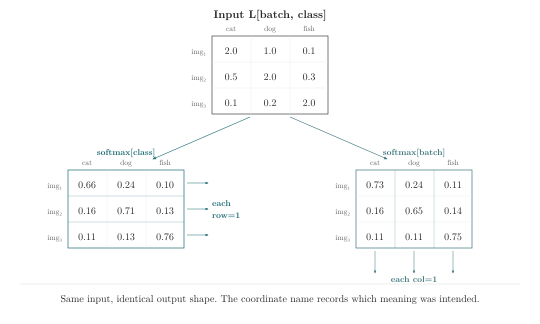
\includegraphics{figures/softmax_roles.pdf}
\caption{The Square Matrix Test: when dimensions have equal extent, only
the coordinate name records which meaning was intended}
\end{figure}

The figure shows the Square Matrix Test applied to softmax. Two
\(3 \times 3\) probability matrices sit side by side, with row labels
(img1, img2, img3) and column labels (cat, dog, fish). The left matrix
was produced by \texttt{softmax{[}class{]}}---every row sums to 1,
meaning each image's class probabilities are normalized against each
other. The right matrix was produced by
\texttt{softmax{[}batch{]}}---every row also sums to 1, but the
normalization ran over examples instead of classes. When
\texttt{batch\_size\ ==\ num\_classes\ ==\ 3}, the two matrices are
numerically identical. The numbers in every cell match. No shape checker
catches this. No gradient check catches this. Only a notation that
records \emph{which coordinate is the distribution} catches this.

Here is softmax over class vs.~softmax over batch, with 3 classes and 3
examples:

\begin{verbatim}
Logits (correct layout [batch, class]):
         cat  dog  fish
  img1: [2.0, 1.0, 0.1]  →  softmax over class → [0.66, 0.24, 0.10]
  img2: [0.5, 2.0, 0.3]  →  softmax over class → [0.14, 0.63, 0.23]
  img3: [0.1, 0.2, 2.0]  →  softmax over class → [0.10, 0.12, 0.78]
  Each row sums to 1.0. This is correct.

Logits (swapped layout [class, batch]):
  img1: [2.0, 1.0, 0.1]  →  softmax over batch → [0.66, 0.24, 0.10]
  img2: [0.5, 2.0, 0.3]  →  softmax over batch → [0.14, 0.63, 0.23]
  img3: [0.1, 0.2, 2.0]  →  softmax over batch → [0.10, 0.12, 0.78]
  Each row sums to 1.0. The numbers are IDENTICAL.
\end{verbatim}

When \texttt{batch\_size\ ==\ num\_classes}, the probability matrix is
square. Softmax over rows and softmax over columns produce the same
numbers when the matrix has symmetric structure. The loss curves
overlay. The calibration reports pass. Six weeks later, a deployed model
silently normalizes examples against each other instead of classes
against each other.

No shape checker catches this. No gradient check catches this. Only a
notation that records \emph{which coordinate is the distribution}
catches this. \texttt{softmax{[}class{]}(logits)} records it.
\texttt{softmax(logits,\ dim=-1)} does not.

In a \texttt{dim=-1} API, these three roles collapse into a single
integer. The reader cannot see which role \texttt{dim=-1} plays at each
step of the decomposition. In the named-coordinate version, the roles
are given distinct letters, and a reader can audit whether the gradient
contracts are satisfied.

\hypertarget{the-square-matrix-test}{%
\subsection{The Square Matrix Test}\label{the-square-matrix-test}}

There is a simple, brutal test for whether a piece of tensor code is
robust to coordinate swaps. Set all dimension sizes equal. Swap two
axes. Ask: does the program still mean the same thing?

For a square input where
\texttt{batch\_size\ ==\ num\_classes\ ==\ 128}:

\begin{Shaded}
\begin{Highlighting}[]
\KeywordTok{let}\NormalTok{ probs}\OperatorTok{[}\NormalTok{batch, class}\OperatorTok{]}\NormalTok{ = softmax}\OperatorTok{[}\NormalTok{class}\OperatorTok{]}\NormalTok{(logits}\OperatorTok{[}\NormalTok{batch, class}\OperatorTok{]}\NormalTok{);   }\CommentTok{// correct}
\KeywordTok{let}\NormalTok{ probs}\OperatorTok{[}\NormalTok{class, batch}\OperatorTok{]}\NormalTok{ = softmax}\OperatorTok{[}\NormalTok{batch}\OperatorTok{]}\NormalTok{(logits}\OperatorTok{[}\NormalTok{class, batch}\OperatorTok{]}\NormalTok{);   }\CommentTok{// bug}
\end{Highlighting}
\end{Shaded}

Both lines produce a \texttt{(128,\ 128)} matrix where every row sums to
1. The cross-entropy loss descends identically. The training curves
overlay perfectly. But the first normalizes classes against each other.
The second normalizes examples against each other. A deployed model
using the second version will produce confidence scores that drift with
batch size.

The Square Matrix Test is named after this property: when all extents
are equal, a coordinate swap can hide inside shape compatibility. The
test asks: if I rename the axes, does the program's \emph{meaning}
change? If so, the renamed axes should be reflected in the source---and
the source should make them visible enough that a rename would break
compilation or at minimum readability.

Apply the Square Matrix Test to any softmax call you write. If
\texttt{softmax{[}class{]}(logits)} would silently become wrong when
\texttt{class} and \texttt{batch} swap, your notation is not recording
the necessary fact.

\hypertarget{the-language-gets-a-name}{%
\subsection{The Language Gets a Name}\label{the-language-gets-a-name}}

We have been writing in a notation that puts coordinate names in
brackets, that requires reductions to state what they consume, that
makes broadcasting explicit in the indexing pattern. This notation needs
a name.

It is called \textbf{einlang}---a contraction of ``Einstein'' and
``language,'' acknowledging the debt to Einstein summation notation
while distinguishing itself as a full programming language rather than a
string-based convention.

The name is not the point. The point is what the name represents: a
language where coordinates are first-class syntactic entities, not
comments embedded in variable names. Where the compiler checks
coordinate contracts. Where the reader can audit coordinate flow without
reconstructing it from shape arithmetic.

Einlang is the microscope. The coordinate habit is the specimen. This
book teaches both.

\begin{center}\rule{0.5\linewidth}{0.4pt}\end{center}

\hypertarget{composition-without-pipelines}{%
\subsection{Composition Without
Pipelines}\label{composition-without-pipelines}}

Some languages use a pipeline operator
(\texttt{\textbar{}\textgreater{}}) to thread data through a sequence of
transformations. Einlang does not need one. \texttt{let} bindings
already express data-flow composition:

\begin{Shaded}
\begin{Highlighting}[]
\KeywordTok{let}\NormalTok{ step1 = normalize}\OperatorTok{[}\NormalTok{feature}\OperatorTok{]}\NormalTok{(raw);}
\KeywordTok{let}\NormalTok{ step2 = activate(step1);}
\KeywordTok{let}\NormalTok{ step3 = project}\OperatorTok{[}\NormalTok{out}\OperatorTok{]}\NormalTok{(step2, weight);}
\end{Highlighting}
\end{Shaded}

Each step names its result. The names serve as documentation. The data
flow is visible in the sequence of bindings. No new syntax is required
because the language's existing means of combination---\texttt{let}
declarations, function calls, coordinate arguments---already compose
cleanly.

This is a deliberate choice. Einlang is a small language. Every
syntactic addition must justify itself against the alternative of using
what's already there. Pipeline operators, in particular, add a new
control-flow concept for a benefit---reading transformations in
execution order---that named \texttt{let} bindings already provide.

\begin{center}\rule{0.5\linewidth}{0.4pt}\end{center}

\hypertarget{what-we-carry-forward}{%
\subsection{What We Carry Forward}\label{what-we-carry-forward}}

This chapter crossed a threshold. Before it, we worked with
primitives---single statements that name, permute, reduce, or broadcast
coordinates. After it, we have a means of combination: the
coordinate-aware function, whose signature declares which coordinates it
consumes, which it preserves, and which it is polymorphic over.

The next three chapters explore what happens when combinations interact:
the traps that refactoring creates (Chapter 7), the mirror world of
gradients (Chapter 8), and the challenge of updating parameters across
time (Chapter 9).

\hypertarget{try-it-5}{%
\subsubsection{Try It}\label{try-it-5}}

\begin{enumerate}
\def\labelenumi{\arabic{enumi}.}
\item
  Rewrite the softmax decomposition as a coordinate-aware function
  \texttt{fn\ my\_softmax{[}coord{]}(x:\ {[}f32;\ ..left,\ coord,\ ..right{]})\ -\textgreater{}\ {[}f32;\ ..left,\ coord,\ ..right{]}}.
  Test it mentally on a 2D tensor \texttt{logits{[}b,\ c{]}} and a 3D
  tensor \texttt{scores{[}b,\ h,\ c{]}}. Does your function work for
  both?
\item
  What happens if you call \texttt{softmax{[}class{]}(logits)} but
  \texttt{logits} has shape \texttt{(32,\ 10)} and has never been bound
  with coordinate names? (Hint: the compiler requires coordinates to be
  grounded. Read the error.)
\item
  A colleague proposes a function
  \texttt{fn\ top1{[}class{]}(x:\ {[}f32;\ ..left,\ class,\ ..right{]})\ -\textgreater{}\ {[}i32;\ ..left,\ ..right{]}}
  that returns the index of the maximum element along \texttt{class}.
  Write its body using \texttt{argmax}. What coordinates survive in the
  result?
\end{enumerate}

\newpage

\hypertarget{chapter-7-the-refactoring-trap}{%
\section{Chapter 7 · The Refactoring
Trap}\label{chapter-7-the-refactoring-trap}}

\begin{quote}
``The first principle is that you must not fool yourself---and you are
the easiest person to fool.''

--- Richard Feynman
\end{quote}

\emph{Combinations · Immutability, where-clause bindings, and boolean
guards}

\begin{center}\rule{0.5\linewidth}{0.4pt}\end{center}

There is a species of refactoring that makes code shorter, cleaner, and
wrong.

It happens when you notice that two branches of an \texttt{if} share a
structure, so you merge them into a single loop. Or when you see a
repeated subexpression and factor it out. Or when you inline a variable
that ``isn't doing anything.''

Each of these is a good instinct. Each of them, applied to tensor code
without coordinate awareness, can silently delete the information that
made the code correct.

This chapter is about the traps that sit between ``it works'' and ``it's
clean.'' The traps are not bugs in the language. They are bugs in the
assumption that shorter code preserves meaning. In a positional
notation, that assumption is frequently false. In a named-coordinate
notation, the syntax itself prevents the most common forms of semantic
collapse.

\begin{center}\rule{0.5\linewidth}{0.4pt}\end{center}

\hypertarget{immutability-the-binding-that-doesnt-change}{%
\subsection{Immutability: The Binding That Doesn't
Change}\label{immutability-the-binding-that-doesnt-change}}

Every \texttt{let} binding in einlang is immutable. Once a name is bound
to a value, that binding cannot be changed within its scope:

\begin{Shaded}
\begin{Highlighting}[]
\KeywordTok{let}\NormalTok{ x = }\DecValTok{10}\NormalTok{;}
\KeywordTok{let}\NormalTok{ x = x + }\DecValTok{1}\NormalTok{;   }\CommentTok{// ERROR: redefinition of `x` in the same scope}
\KeywordTok{let}\NormalTok{ x_next = x + }\DecValTok{1}\NormalTok{;   }\CommentTok{// OK: new name}
\end{Highlighting}
\end{Shaded}

This is not a stylistic preference. It is a semantic guarantee that
serves the coordinate audit. When you see \texttt{x{[}b,\ c{]}} on line
50 and trace it back to its definition on line 10, you know that
\texttt{x} still means what it meant on line 10. There is no mutation
that could have changed its shape, its coordinates, or its values
between definition and use.

In a language with mutable variables, refactoring often introduces bugs
by accidentally rebinding a name to a tensor with a different coordinate
layout. You had \texttt{x} as \texttt{(batch,\ channel,\ spatial)};
later someone inserts \texttt{x\ =\ x.transpose(1,\ 2)}. The name
\texttt{x} now points to a tensor with a different axis order. All
downstream code that assumed the original order is now silently wrong.
The shapes might even match, if \texttt{channel} and \texttt{spatial}
happen to have the same size.

Immutability eliminates this class of bug entirely. A \texttt{let}
binding is a definition, not an assignment. It states a fact. Facts
don't change.

\begin{center}\rule{0.5\linewidth}{0.4pt}\end{center}

\hypertarget{the-where-clause-naming-without-cluttering}{%
\subsection{The Where Clause: Naming Without
Cluttering}\label{the-where-clause-naming-without-cluttering}}

Chapter 5 introduced the \texttt{where} clause for boolean guards. But
the where clause has a second, equally important role: it provides a
scoped space for intermediate variables that are only relevant to a
single declaration:

\begin{Shaded}
\begin{Highlighting}[]
\KeywordTok{let}\NormalTok{ output}\OperatorTok{[}\NormalTok{i, j}\OperatorTok{]}\NormalTok{ = activated}
    \KeywordTok{where}\NormalTok{ z = sum}\OperatorTok{[}\NormalTok{k}\OperatorTok{]}\NormalTok{(input}\OperatorTok{[}\NormalTok{i, k}\OperatorTok{]}\NormalTok{ * weight}\OperatorTok{[}\NormalTok{k, j}\OperatorTok{]}\NormalTok{) + bias}\OperatorTok{[}\NormalTok{j}\OperatorTok{]}\NormalTok{,}
\NormalTok{          activated = }\KeywordTok{if}\NormalTok{ z > }\DecValTok{0.0} \OperatorTok{\{}\NormalTok{ z }\OperatorTok{\}} \KeywordTok{else} \OperatorTok{\{} \DecValTok{0.0} \OperatorTok{\}}\NormalTok{;}
\end{Highlighting}
\end{Shaded}

Without the where clause, you face a choice. Either you repeat the
\texttt{sum{[}k{]}(...)} expression:

\begin{Shaded}
\begin{Highlighting}[]
\CommentTok{// Bad: duplicated computation, and the two copies can drift apart}
\KeywordTok{let}\NormalTok{ output}\OperatorTok{[}\NormalTok{i, j}\OperatorTok{]}\NormalTok{ = }\KeywordTok{if}\NormalTok{ sum}\OperatorTok{[}\NormalTok{k}\OperatorTok{]}\NormalTok{(input}\OperatorTok{[}\NormalTok{i, k}\OperatorTok{]}\NormalTok{ * weight}\OperatorTok{[}\NormalTok{k, j}\OperatorTok{]}\NormalTok{) + bias}\OperatorTok{[}\NormalTok{j}\OperatorTok{]}\NormalTok{ > }\DecValTok{0.0}
    \OperatorTok{\{}\NormalTok{ sum}\OperatorTok{[}\NormalTok{k}\OperatorTok{]}\NormalTok{(input}\OperatorTok{[}\NormalTok{i, k}\OperatorTok{]}\NormalTok{ * weight}\OperatorTok{[}\NormalTok{k, j}\OperatorTok{]}\NormalTok{) + bias}\OperatorTok{[}\NormalTok{j}\OperatorTok{]} \OperatorTok{\}}
    \KeywordTok{else} \OperatorTok{\{} \DecValTok{0.0} \OperatorTok{\}}\NormalTok{;}
\end{Highlighting}
\end{Shaded}

Or you introduce a temporary tensor that exists at the scope level:

\begin{Shaded}
\begin{Highlighting}[]
\CommentTok{// Better, but `z` now lives in the outer scope}
\KeywordTok{let}\NormalTok{ z}\OperatorTok{[}\NormalTok{i, j}\OperatorTok{]}\NormalTok{ = sum}\OperatorTok{[}\NormalTok{k}\OperatorTok{]}\NormalTok{(input}\OperatorTok{[}\NormalTok{i, k}\OperatorTok{]}\NormalTok{ * weight}\OperatorTok{[}\NormalTok{k, j}\OperatorTok{]}\NormalTok{) + bias}\OperatorTok{[}\NormalTok{j}\OperatorTok{]}\NormalTok{;}
\KeywordTok{let}\NormalTok{ output}\OperatorTok{[}\NormalTok{i, j}\OperatorTok{]}\NormalTok{ = }\KeywordTok{if}\NormalTok{ z}\OperatorTok{[}\NormalTok{i, j}\OperatorTok{]}\NormalTok{ > }\DecValTok{0.0} \OperatorTok{\{}\NormalTok{ z}\OperatorTok{[}\NormalTok{i, j}\OperatorTok{]} \OperatorTok{\}} \KeywordTok{else} \OperatorTok{\{} \DecValTok{0.0} \OperatorTok{\}}\NormalTok{;}
\end{Highlighting}
\end{Shaded}

The where clause gives you a third option: name the intermediate value,
but keep it lexically scoped to the declaration that needs it.
\texttt{z} and \texttt{activated} exist only within the where clause.
They do not clutter the outer scope. The reader knows they are
implementation details of this one declaration, not structural values
that other code depends on.

This is a small syntactic feature with an outsized impact on refactoring
safety. When you extract a computation into a where-clause binding, you
are not changing the scope of any name visible to other code. You are
localizing the change. Local changes are easier to audit.

\begin{center}\rule{0.5\linewidth}{0.4pt}\end{center}

\hypertarget{boolean-guards-filtering-without-masks}{%
\subsection{Boolean Guards: Filtering Without
Masks}\label{boolean-guards-filtering-without-masks}}

A boolean guard in a where clause filters the domain over which the
declaration applies:

\begin{Shaded}
\begin{Highlighting}[]
\KeywordTok{let}\NormalTok{ pos_sum = sum}\OperatorTok{[}\NormalTok{i}\OperatorTok{]}\NormalTok{(data}\OperatorTok{[}\NormalTok{i}\OperatorTok{]}\NormalTok{) }\KeywordTok{where}\NormalTok{ data}\OperatorTok{[}\NormalTok{i}\OperatorTok{]}\NormalTok{ > }\DecValTok{0}\NormalTok{;}
\KeywordTok{let}\NormalTok{ upper}\OperatorTok{[}\NormalTok{i, j}\OperatorTok{]}\NormalTok{ = matrix}\OperatorTok{[}\NormalTok{i, j}\OperatorTok{]} \KeywordTok{where}\NormalTok{ i <= j;}
\end{Highlighting}
\end{Shaded}

These read like set comprehensions: ``sum over \texttt{i} such that
\texttt{data{[}i{]}} is positive.'' No mask tensor is created. No
broadcasting semantics need to be verified. The guard operates on the
index variables directly.

In a positional framework, you'd write:

\begin{Shaded}
\begin{Highlighting}[]
\NormalTok{mask }\OperatorTok{=}\NormalTok{ data }\OperatorTok{>} \DecValTok{0}
\NormalTok{pos_sum }\OperatorTok{=}\NormalTok{ (data }\OperatorTok{*}\NormalTok{ mask).}\BuiltInTok{sum}\NormalTok{()}
\end{Highlighting}
\end{Shaded}

This creates a temporary tensor \texttt{mask}. It relies on broadcasting
to align \texttt{mask} with \texttt{data}. If \texttt{data} has an
unexpected batch dimension, the mask silently broadcasts into it. If you
later refactor to remove the temporary, you might accidentally change
the broadcasting behavior.

The where clause avoids all of this by attaching the filter to the
reduction syntactically. The filter's domain is the reduction's domain.
There is no separate mask whose shape must be audited.

\begin{center}\rule{0.5\linewidth}{0.4pt}\end{center}

\hypertarget{refactoring-with-names}{%
\subsection{Refactoring with Names}\label{refactoring-with-names}}

Let's put these pieces together. A common refactoring is to take a
repeated pattern and extract it into a function. Here is the before, in
positional PyTorch:

\begin{Shaded}
\begin{Highlighting}[]
\CommentTok{# Before: two instances of the same pattern}
\NormalTok{h1 }\OperatorTok{=}\NormalTok{ torch.relu(torch.matmul(x, W1) }\OperatorTok{+}\NormalTok{ b1)}
\NormalTok{h2 }\OperatorTok{=}\NormalTok{ torch.relu(torch.matmul(x, W2) }\OperatorTok{+}\NormalTok{ b2)}
\end{Highlighting}
\end{Shaded}

A clean refactoring would extract the linear-relu pattern:

\begin{Shaded}
\begin{Highlighting}[]
\KeywordTok{def}\NormalTok{ linear_relu(x, W, b):}
    \ControlFlowTok{return}\NormalTok{ torch.relu(torch.matmul(x, W) }\OperatorTok{+}\NormalTok{ b)}
\end{Highlighting}
\end{Shaded}

What information was lost? The coordinate structure.
\texttt{torch.matmul(x,\ W)} contracts the last dimension of \texttt{x}
with the second-to-last of \texttt{W}. Which coordinate is that? The
function signature doesn't say. The caller has to know that \texttt{x}
must end with the input-feature dimension and \texttt{W} must have
output-feature followed by input-feature. If either convention changes,
every call site silently breaks.

Now in einlang:

\begin{Shaded}
\begin{Highlighting}[]
\KeywordTok{fn}\NormalTok{ linear_relu[in](x: }\OperatorTok{[}\DataTypeTok{f32}\NormalTok{; ..batch, }\KeywordTok{in}\OperatorTok{]}\NormalTok{, W: }\OperatorTok{[}\DataTypeTok{f32}\NormalTok{; out, }\KeywordTok{in}\OperatorTok{]}\NormalTok{, b: }\OperatorTok{[}\DataTypeTok{f32}\NormalTok{; out}\OperatorTok{]}\NormalTok{)}
\NormalTok{    -> }\OperatorTok{[}\DataTypeTok{f32}\NormalTok{; ..batch, out}\OperatorTok{]}
\OperatorTok{\{}
    \KeywordTok{let}\NormalTok{ z}\OperatorTok{[}\NormalTok{..batch, out}\OperatorTok{]}\NormalTok{ = sum}\OperatorTok{[}\KeywordTok{in}\OperatorTok{]}\NormalTok{(x}\OperatorTok{[}\NormalTok{..batch, }\KeywordTok{in}\OperatorTok{]}\NormalTok{ * W}\OperatorTok{[}\NormalTok{out, }\KeywordTok{in}\OperatorTok{]}\NormalTok{) + b}\OperatorTok{[}\NormalTok{out}\OperatorTok{]}\NormalTok{;}
    \KeywordTok{if}\NormalTok{ z}\OperatorTok{[}\NormalTok{..batch, out}\OperatorTok{]}\NormalTok{ > }\DecValTok{0.0} \OperatorTok{\{}\NormalTok{ z}\OperatorTok{[}\NormalTok{..batch, out}\OperatorTok{]} \OperatorTok{\}} \KeywordTok{else} \OperatorTok{\{} \DecValTok{0.0} \OperatorTok{\}}
\OperatorTok{\}}
\end{Highlighting}
\end{Shaded}

The coordinate \texttt{in} is a coordinate parameter---it names the
contracted dimension. The coordinate \texttt{out} appears in
\texttt{W}'s shape and the return type. The rest pack \texttt{..batch}
handles whatever batch structure the caller provides. The coordinate
contract is in the type signature. The compiler checks it at every call
site. The refactoring did not hide anything, because the syntax had a
place to put the facts.

\begin{center}\rule{0.5\linewidth}{0.4pt}\end{center}

When you refactor, you are making a bet: that the new, shorter code is
equivalent to the old, longer code. In a positional notation, verifying
that bet requires holding the coordinate story in your head while
comparing two versions of the code. In a named-coordinate notation, the
coordinate story is part of the text you're comparing. The bet is easier
to verify because the evidence is on the page.

Next chapter: the gradient. When the forward pass eliminates a
coordinate, the backward pass must recover it. We'll see how the
coordinate contract extends naturally into differentiation.

\hypertarget{try-it-6}{%
\subsubsection{Try It}\label{try-it-6}}

\begin{enumerate}
\def\labelenumi{\arabic{enumi}.}
\tightlist
\item
  Refactor the following into a single declaration with a where clause.
  Does your version still clearly state which coordinates survive and
  which are consumed?
\end{enumerate}

\begin{Shaded}
\begin{Highlighting}[]
\KeywordTok{let}\NormalTok{ scores}\OperatorTok{[}\NormalTok{b, i, j}\OperatorTok{]}\NormalTok{ = sum}\OperatorTok{[}\NormalTok{d}\OperatorTok{]}\NormalTok{(Q}\OperatorTok{[}\NormalTok{b, i, d}\OperatorTok{]}\NormalTok{ * K}\OperatorTok{[}\NormalTok{b, j, d}\OperatorTok{]}\NormalTok{);}
\KeywordTok{let}\NormalTok{ weights}\OperatorTok{[}\NormalTok{b, i, j}\OperatorTok{]}\NormalTok{ = softmax}\OperatorTok{[}\NormalTok{j}\OperatorTok{]}\NormalTok{(scores}\OperatorTok{[}\NormalTok{b, i, j}\OperatorTok{]}\NormalTok{);}
\KeywordTok{let}\NormalTok{ output}\OperatorTok{[}\NormalTok{b, i, d}\OperatorTok{]}\NormalTok{ = sum}\OperatorTok{[}\NormalTok{j}\OperatorTok{]}\NormalTok{(weights}\OperatorTok{[}\NormalTok{b, i, j}\OperatorTok{]}\NormalTok{ * V}\OperatorTok{[}\NormalTok{b, j, d}\OperatorTok{]}\NormalTok{);}
\end{Highlighting}
\end{Shaded}

\begin{enumerate}
\def\labelenumi{\arabic{enumi}.}
\setcounter{enumi}{1}
\item
  A colleague argues that \texttt{let} immutability is ``annoying''
  because it forces them to invent new names for every intermediate
  tensor. Write a one-paragraph response. What does immutability buy you
  during a refactoring, specifically when coordinate layouts might
  change?
\item
  In the boolean guard
  \texttt{let\ upper{[}i,\ j{]}\ =\ matrix{[}i,\ j{]}\ where\ i\ \textless{}=\ j;},
  what happens to positions where \texttt{i\ \textgreater{}\ j}? What
  value do they take in the output tensor?
\end{enumerate}

\newpage

\hypertarget{chapter-8-the-challenge-of-walking-backward}{%
\section{Chapter 8 · The Challenge of Walking
Backward}\label{chapter-8-the-challenge-of-walking-backward}}

\begin{quote}
``In the forward pass, you eliminate information. In the backward pass,
you guess.''

--- The author, after a long debugging session
\end{quote}

\emph{Combinations, mirrored · Automatic differentiation}

\begin{center}\rule{0.5\linewidth}{0.4pt}\end{center}

Chapter 5 introduced \texttt{@y\ /\ @x} as a diagnostic tool for
broadcast contracts. We used it in the simplest possible
setting---scalar derivatives---to verify that our forward broadcasts
produced the expected backward reductions.

This chapter goes deeper. We trace gradients through matrix
multiplication, through convolution, through functions we define
ourselves. At each step, the coordinate names tell the story of what the
gradient must sum over---and what happens when the names are wrong.

\begin{center}\rule{0.5\linewidth}{0.4pt}\end{center}

\hypertarget{the-gradient-as-coordinate-subtraction}{%
\subsection{The Gradient as Coordinate
Subtraction}\label{the-gradient-as-coordinate-subtraction}}

A derivative measures sensitivity. \texttt{@loss\ /\ @W} asks: if I
perturb \texttt{W} by a small amount, how much does \texttt{loss}
change? For scalar \texttt{loss} and scalar \texttt{W}, the answer is a
single number. For tensor \texttt{W}, the answer is a tensor of the same
shape as \texttt{W}---each element says how \texttt{loss} responds to
perturbing that specific element.

This means the shape of \texttt{@loss\ /\ @W} is the shape of
\texttt{W}. The set of coordinates on the result of differentiation is
exactly the set of coordinates on the denominator.

But \texttt{loss} is a scalar---it has no coordinates. So the path from
\texttt{W} to \texttt{loss} must eliminate every coordinate that
\texttt{W} carries. The gradient computation must reconstruct those
eliminations in reverse: every forward reduction becomes a backward
broadcast, and every forward broadcast becomes a backward reduction.

Let's trace this for matrix multiplication.

\begin{center}\rule{0.5\linewidth}{0.4pt}\end{center}

\begin{figure}
\centering
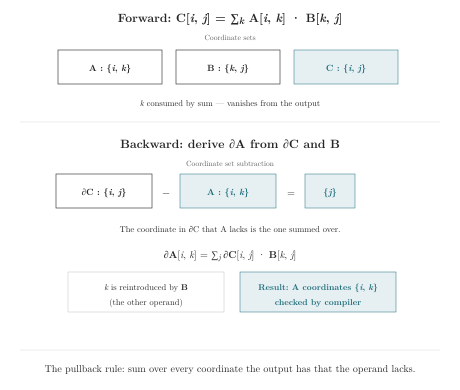
\includegraphics{figures/gradient_pullback.pdf}
\caption{Forward and backward: the gradient sums over coordinates in C
but not in A}
\end{figure}

The figure traces the full round trip. Top half (Forward): matrices
\(\mathbf{A}\) and \(\mathbf{B}\) feed into \(\mathbf{C}\) through a
\texttt{sum{[}k{]}} reduction. The coordinate sets are annotated:
\(\mathbf{A} : \{i,k\}\), \(\mathbf{B} : \{k,j\}\),
\(\mathbf{C} : \{i,j\}\). The divider marks the reversal. Bottom half
(Backward): the incoming gradient \(\partial\mathbf{C}\) (with
coordinates \(\{i,j\}\)) and the operand \(\mathbf{B}\) (with
\(\{k,j\}\)) feed into \(\partial\mathbf{A}\) (with \(\{i,k\}\)). The
set subtraction rule is written out:
\(\mathbf{C}\{i,j\} \setminus \mathbf{A}\{i,k\} = \{j\}\). The
coordinate \(j\)---present in \(\mathbf{C}\) but absent from
\(\mathbf{A}\)---is the one summed over. The coordinate \(k\)---absent
from \(\mathbf{C}\) but present in \(\mathbf{A}\)---is reintroduced by
\(\mathbf{B}\). This is not a special case for matrix multiplication. It
is the universal pullback rule for sum-of-products: sum over what the
output has that the operand lacks.

\hypertarget{the-matmul-pullback}{%
\subsection{The Matmul Pullback}\label{the-matmul-pullback}}

Forward pass:

\begin{Shaded}
\begin{Highlighting}[]
\KeywordTok{let}\NormalTok{ C}\OperatorTok{[}\NormalTok{i, j}\OperatorTok{]}\NormalTok{ = sum}\OperatorTok{[}\NormalTok{k}\OperatorTok{]}\NormalTok{(A}\OperatorTok{[}\NormalTok{i, k}\OperatorTok{]}\NormalTok{ * B}\OperatorTok{[}\NormalTok{k, j}\OperatorTok{]}\NormalTok{);}
\end{Highlighting}
\end{Shaded}

\texttt{C} has coordinates \texttt{{[}i,\ j{]}}. \texttt{A} has
\texttt{{[}i,\ k{]}}. \texttt{B} has \texttt{{[}k,\ j{]}}. The
coordinate \texttt{k} is consumed by the reduction.

Now suppose we have \texttt{dC{[}i,\ j{]}}---the gradient of the loss
with respect to \texttt{C}. We want \texttt{@C\ /\ @A} and
\texttt{@C\ /\ @B}.

For \texttt{@C\ /\ @A}: the result must have coordinates
\texttt{{[}i,\ k{]}} (the coordinates of \texttt{A}). The gradient
signal \texttt{dC} has coordinates \texttt{{[}i,\ j{]}}. We need to
eliminate \texttt{j} and introduce \texttt{k}. Which operation does
that? Multiply \texttt{dC{[}i,\ j{]}} by the \emph{other} input
\texttt{B{[}k,\ j{]}}, and sum over \texttt{j}:

\begin{Shaded}
\begin{Highlighting}[]
\KeywordTok{let}\NormalTok{ dA}\OperatorTok{[}\NormalTok{i, k}\OperatorTok{]}\NormalTok{ = sum}\OperatorTok{[}\NormalTok{j}\OperatorTok{]}\NormalTok{(dC}\OperatorTok{[}\NormalTok{i, j}\OperatorTok{]}\NormalTok{ * B}\OperatorTok{[}\NormalTok{k, j}\OperatorTok{]}\NormalTok{);}
\end{Highlighting}
\end{Shaded}

The sum coordinate is \texttt{j}---the coordinate that \texttt{A} does
not have but \texttt{C} does. The surviving coordinates are \texttt{i}
(shared between \texttt{A} and \texttt{C}) and \texttt{k} (from
\texttt{A}, reintroduced by \texttt{B}).

This is the pullback rule: \textbf{the gradient sums over the
set-difference of coordinates between the output and the operand.}
\texttt{C} has \texttt{\{i,\ j\}}. \texttt{A} has \texttt{\{i,\ k\}}.
The difference is \texttt{\{j\}} minus \texttt{\{k\}}---we sum over
\texttt{j} and \texttt{k} is provided by \texttt{B}.

You don't need to memorize the formula for a matmul pullback. You need
the coordinate accounting. Which coordinates does the operand carry?
Which does the output carry? The reduction coordinates in the gradient
are exactly the coordinates present in the output but absent from the
operand.

This rule is general. It works for any sum-of-products expression, not
just matrix multiplication. It works for convolutions, for bilinear
layers, for attention score computations. The coordinates tell you what
to sum over. The rest is just multiplication with the other operands.

\begin{center}\rule{0.5\linewidth}{0.4pt}\end{center}

\hypertarget{the-five-step-pullback-procedure}{%
\subsection{The Five-Step Pullback
Procedure}\label{the-five-step-pullback-procedure}}

The pullback rule of Chapter 7 can be turned into a mechanical
procedure. Given a forward expression and a target operand, derive the
gradient:

\begin{enumerate}
\def\labelenumi{\arabic{enumi}.}
\tightlist
\item
  \textbf{Hold one cell} of the target operand. Choose a specific
  element---say \texttt{A{[}i₀,\ k₀{]}}.
\item
  \textbf{List every output cell that reads it.} For
  \texttt{C{[}i,\ j{]}\ =\ sum{[}k{]}(A{[}i,\ k{]}\ *\ B{[}k,\ j{]})},
  the held cell \texttt{A{[}i₀,\ k₀{]}} is read by every output where
  \texttt{i\ =\ i₀} and the sum includes \texttt{k\ =\ k₀}. That means
  \texttt{C{[}i₀,\ j{]}} for \emph{all} \texttt{j}.
\item
  \textbf{Attach the incoming gradient.} Each output cell
  \texttt{C{[}i₀,\ j{]}} carries a gradient signal
  \texttt{dC{[}i₀,\ j{]}}. The contribution from the path through
  \texttt{A{[}i₀,\ k₀{]}} is \texttt{dC{[}i₀,\ j{]}\ *\ B{[}k₀,\ j{]}}.
\item
  \textbf{Multiply by the local derivative.} For elementwise
  multiplication inside the sum, the local derivative of
  \texttt{A{[}i,\ k{]}\ *\ B{[}k,\ j{]}} with respect to
  \texttt{A{[}i,\ k{]}} is \texttt{B{[}k,\ j{]}}. So the total
  sensitivity at \texttt{A{[}i₀,\ k₀{]}} is
  \texttt{sum{[}j{]}(dC{[}i₀,\ j{]}\ *\ B{[}k₀,\ j{]})}.
\item
  \textbf{Sum the routes.} The path coordinate---the coordinate in
  \texttt{C} but not in \texttt{A}---is \texttt{j}. Sum over it.
\end{enumerate}

The result:
\texttt{dA{[}i,\ k{]}\ =\ sum{[}j{]}(dC{[}i,\ j{]}\ *\ B{[}k,\ j{]})}.
No calculus memorization. No transpose rules. Just coordinate
accounting.

This procedure works for \emph{any} sum-of-products expression in
einlang. For convolution, the same five steps produce the weight
gradient with the correct index arithmetic. The coordinate set
subtraction is the engine. The five steps are the manual.

\begin{center}\rule{0.5\linewidth}{0.4pt}\end{center}

\hypertarget{convolution-gradients}{%
\subsection{Convolution Gradients}\label{convolution-gradients}}

A convolution is a sum of products, just like matrix multiplication, but
with index arithmetic:

\begin{Shaded}
\begin{Highlighting}[]
\KeywordTok{let}\NormalTok{ conv}\OperatorTok{[}\NormalTok{b, oc, oh, ow}\OperatorTok{]}\NormalTok{ = sum}\OperatorTok{[}\NormalTok{ic, kh, kw}\OperatorTok{]}\NormalTok{(}
\NormalTok{    input}\OperatorTok{[}\NormalTok{b, ic, oh + kh, ow + kw}\OperatorTok{]}\NormalTok{ * weight}\OperatorTok{[}\NormalTok{oc, ic, kh, kw}\OperatorTok{]}
\NormalTok{);}
\end{Highlighting}
\end{Shaded}

The gradient with respect to \texttt{weight} sums over everything that
\texttt{weight} does not own:

\begin{Shaded}
\begin{Highlighting}[]
\KeywordTok{let}\NormalTok{ dW}\OperatorTok{[}\NormalTok{oc, ic, kh, kw}\OperatorTok{]}\NormalTok{ = sum}\OperatorTok{[}\NormalTok{b, oh, ow}\OperatorTok{]}\NormalTok{(}
\NormalTok{    dConv}\OperatorTok{[}\NormalTok{b, oc, oh, ow}\OperatorTok{]}\NormalTok{ * input}\OperatorTok{[}\NormalTok{b, ic, oh + kh, ow + kw}\OperatorTok{]}
\NormalTok{);}
\end{Highlighting}
\end{Shaded}

The coordinates \texttt{b}, \texttt{oh}, \texttt{ow} are summed away
because they appear in the output but not in \texttt{weight}. The
coordinates \texttt{oc}, \texttt{ic}, \texttt{kh}, \texttt{kw} survive
because they \emph{are} \texttt{weight}'s coordinates.

Again: set subtraction. The formula is mechanically derivable from the
coordinate sets.

\begin{center}\rule{0.5\linewidth}{0.4pt}\end{center}

\hypertarget{custom-differentiation-with-fn}{%
\subsection{\texorpdfstring{Custom Differentiation with
\texttt{@fn}}{Custom Differentiation with @fn}}\label{custom-differentiation-with-fn}}

Some functions have derivatives that are better expressed directly than
derived by the compiler. Einlang supports custom derivative rules with
\texttt{@fn}:

\begin{Shaded}
\begin{Highlighting}[]
\KeywordTok{fn}\NormalTok{ relu(x) }\OperatorTok{\{} \KeywordTok{if}\NormalTok{ x > }\DecValTok{0.0} \OperatorTok{\{}\NormalTok{ x }\OperatorTok{\}} \KeywordTok{else} \OperatorTok{\{} \DecValTok{0.0} \OperatorTok{\}} \OperatorTok{\}}

\NormalTok{@fn relu(x) }\OperatorTok{\{}
    \KeywordTok{if}\NormalTok{ x > }\DecValTok{0.0} \OperatorTok{\{}\NormalTok{ @x }\OperatorTok{\}} \KeywordTok{else} \OperatorTok{\{} \DecValTok{0.0} \OperatorTok{\}}
\OperatorTok{\}}
\end{Highlighting}
\end{Shaded}

The \texttt{@fn} declaration shares the function's name and parameter
list. Inside the body, \texttt{@x} refers to the tangent flowing through
parameter \texttt{x}. The body describes how to assemble the output
tangent from the input tangents.

Custom rules can also be coordinate-aware:

\begin{Shaded}
\begin{Highlighting}[]
\NormalTok{@fn softmax}\OperatorTok{[}\NormalTok{j}\OperatorTok{]}\NormalTok{(x: }\OperatorTok{[}\DataTypeTok{f32}\NormalTok{; ..left, j, ..right}\OperatorTok{]}\NormalTok{) }\OperatorTok{\{}
\NormalTok{    softmax_tangent}\OperatorTok{[}\NormalTok{j}\OperatorTok{]}\NormalTok{(x, @x)}
\OperatorTok{\}}
\end{Highlighting}
\end{Shaded}

The coordinate parameter \texttt{j} appears in both the primal function
and its derivative rule. The tangent computation follows the same
coordinate contract as the primal.

Custom rules are useful when: - The function calls external code
(Python/NumPy) whose internals the compiler can't trace. - You want a
surrogate derivative---for example, a straight-through estimator that
passes the gradient through a discrete operation. - The derivative is
simpler to write by hand than to let the compiler derive (rare, but it
happens).

\begin{center}\rule{0.5\linewidth}{0.4pt}\end{center}

\hypertarget{recurrence-and-gradients}{%
\subsection{Recurrence and Gradients}\label{recurrence-and-gradients}}

A recurrence defines a sequence where later elements depend on earlier
ones:

\begin{Shaded}
\begin{Highlighting}[]
\KeywordTok{let}\NormalTok{ fib}\OperatorTok{[}\DecValTok{0}\OperatorTok{]}\NormalTok{ = }\DecValTok{0}\NormalTok{;}
\KeywordTok{let}\NormalTok{ fib}\OperatorTok{[}\DecValTok{1}\OperatorTok{]}\NormalTok{ = }\DecValTok{1}\NormalTok{;}
\KeywordTok{let}\NormalTok{ fib}\OperatorTok{[}\NormalTok{n }\KeywordTok{in} \DecValTok{2.}\NormalTok{.}\DecValTok{8}\OperatorTok{]}\NormalTok{ = fib}\OperatorTok{[}\NormalTok{n-}\DecValTok{1}\OperatorTok{]}\NormalTok{ + fib}\OperatorTok{[}\NormalTok{n-}\DecValTok{2}\OperatorTok{]}\NormalTok{;}
\end{Highlighting}
\end{Shaded}

The gradient of a recurrence is itself a recurrence, running backward in
time. If you differentiate \texttt{fib{[}7{]}} with respect to
\texttt{fib{[}0{]}}, the compiler automatically constructs the backward
recurrence that propagates the tangent from \texttt{n=7} back to
\texttt{n=0}. The same coordinate names serve both
directions---\texttt{n} steps forward, and the gradient steps backward
along \texttt{n}.

We'll explore recurrence in depth in Chapter 11. For now, the key
insight: \textbf{the coordinate structure of a recurrence determines the
coordinate structure of its gradient.} Forward and backward share the
same index domain. The same bracket syntax serves both.

\begin{center}\rule{0.5\linewidth}{0.4pt}\end{center}

\hypertarget{where-clauses-in-the-backward-pass}{%
\subsection{Where Clauses in the Backward
Pass}\label{where-clauses-in-the-backward-pass}}

A where clause in the forward pass affects the backward pass. Consider:

\begin{Shaded}
\begin{Highlighting}[]
\KeywordTok{let}\NormalTok{ pos_sum = sum}\OperatorTok{[}\NormalTok{i}\OperatorTok{]}\NormalTok{(data}\OperatorTok{[}\NormalTok{i}\OperatorTok{]}\NormalTok{) }\KeywordTok{where}\NormalTok{ data}\OperatorTok{[}\NormalTok{i}\OperatorTok{]}\NormalTok{ > }\DecValTok{0}\NormalTok{;}
\end{Highlighting}
\end{Shaded}

In the forward pass, only positive elements are summed. In the backward
pass, the gradient signal is distributed only to the positive elements.
Elements that were filtered out receive zero gradient. The where clause
acts as a gate in both directions---forward filtering, backward masking.

The consistency is automatic. You don't write a separate backward
filter. The where clause defines the domain of the operation, and the
domain applies in both directions.

\begin{center}\rule{0.5\linewidth}{0.4pt}\end{center}

The gradient is not a separate computation from the forward pass. It is
the forward pass, read backward. The coordinate names that organize the
forward pass---which survive, which are consumed, which are
omitted---organize the backward pass in exactly the same way. A
coordinate eliminated by a forward sum becomes a coordinate introduced
by a backward broadcast. A coordinate omitted by a forward broadcast
becomes a coordinate summed by a backward reduction.

The names are the same. The direction is reversed. The principle is
symmetric.

\hypertarget{try-it-7}{%
\subsubsection{Try It}\label{try-it-7}}

\begin{enumerate}
\def\labelenumi{\arabic{enumi}.}
\item
  Given
  \texttt{let\ C{[}i,\ j{]}\ =\ sum{[}k{]}(A{[}i,\ k{]}\ *\ B{[}k,\ j{]});},
  derive the gradient \texttt{dC\_dB} using set subtraction. Verify your
  result by checking that the surviving coordinates match \texttt{B}'s
  coordinates \texttt{{[}k,\ j{]}}.
\item
  Write a custom \texttt{@fn} rule for
  \texttt{fn\ square(x)\ \{\ x\ *\ x\ \}}. The derivative should be
  \texttt{2.0\ *\ x\ *\ @x}. Test it mentally: if \texttt{x\ =\ 3.0},
  what is \texttt{@square(x)\ /\ @x}?
\item
  A convolution
  \texttt{let\ y{[}b,\ o,\ i,\ j{]}\ =\ sum{[}c,\ kh,\ kw{]}(x{[}b,\ c,\ i+kh,\ j+kw{]}\ *\ W{[}o,\ c,\ kh,\ kw{]})}
  has forward coordinates \texttt{{[}b,\ o,\ i,\ j{]}} and weight
  coordinates \texttt{{[}o,\ c,\ kh,\ kw{]}}. What coordinates must the
  weight gradient sum over? Why?
\end{enumerate}

\newpage

\hypertarget{chapter-9-updates-with-names}{%
\section{Chapter 9 · Updates, with
Names}\label{chapter-9-updates-with-names}}

\begin{quote}
``The only way to make sense of change is to plunge into it, move with
it, and join the dance.''

--- Alan Watts
\end{quote}

\emph{Combinations · Parameter updates and recurrence syntax}

\begin{center}\rule{0.5\linewidth}{0.4pt}\end{center}

A trained model is a collection of parameter tensors whose values have
been adjusted by an optimizer. The optimizer's job is to nudge each
parameter in the direction that reduces the loss. Which direction? That
depends on the parameter's shape, its coordinate names, and the
gradient's coordinate structure.

This chapter is about the intersection of optimization and coordinate
names. When a weight decay regularizer pushes all values toward zero, it
should push uniformly across the \emph{feature} dimension but not across
the \emph{output} dimension. When an optimizer normalizes gradients by
their variance, it should normalize within each \emph{layer}, not across
layers. These distinctions are invisible in a parameter tensor named
\texttt{w} with shape \texttt{(128,\ 64)}. They become visible when the
tensor carries coordinate names.

\begin{center}\rule{0.5\linewidth}{0.4pt}\end{center}

\hypertarget{parameters-vs.hyperparameters}{%
\subsection{Parameters
vs.~Hyperparameters}\label{parameters-vs.hyperparameters}}

Einlang distinguishes between two kinds of named values:

\begin{Shaded}
\begin{Highlighting}[]
\KeywordTok{let}\NormalTok{ weight: }\OperatorTok{[}\DataTypeTok{f32}\NormalTok{; out, }\KeywordTok{in}\OperatorTok{]}\NormalTok{ = init_random(out, }\KeywordTok{in}\NormalTok{);}
\KeywordTok{let}\NormalTok{ learning_rate: }\DataTypeTok{f32}\NormalTok{ = }\DecValTok{0.001}\NormalTok{;}
\end{Highlighting}
\end{Shaded}

Both are immutable bindings. Both are in scope for subsequent code. But
they have different roles in the optimization story. \texttt{weight} is
a parameter---its value changes during training, driven by gradients.
\texttt{learning\_rate} is a hyperparameter---it controls the
optimizer's behavior but is not itself updated by gradients.

In einlang, the distinction is semantic rather than syntactic. Both use
\texttt{let}. The convention is that parameters carry tensor types with
coordinate names, while hyperparameters are scalars or small
configuration tensors. The coordinate names on parameters serve as
documentation for the optimizer: \texttt{weight{[}out,\ in{]}} tells you
that the first axis corresponds to output neurons and the second to
input neurons. A weight decay regularizer that treats all elements
uniformly can apply without coordinate awareness, but a per-layer or
per-neuron regularization policy needs to know which axis is which.

This is not a language feature. It is a naming discipline. But the
discipline is only possible because the language provides a place to put
the names. When your tensor framework only records shapes, you can't
name the axes; when you can't name the axes, you can't write a
regularizer that distinguishes them.

\begin{center}\rule{0.5\linewidth}{0.4pt}\end{center}

\hypertarget{recurrence-for-parameter-updates}{%
\subsection{Recurrence for Parameter
Updates}\label{recurrence-for-parameter-updates}}

Training is inherently sequential. You compute a forward pass, compute a
loss, compute gradients, and update parameters---then repeat. The
repetition has a time structure. In einlang, that structure is expressed
with \textbf{recurrence declarations}:

\begin{Shaded}
\begin{Highlighting}[]
\KeywordTok{let}\NormalTok{ w}\OperatorTok{[}\DecValTok{0}\NormalTok{, out, }\KeywordTok{in}\OperatorTok{]}\NormalTok{ = init_random(out, }\KeywordTok{in}\NormalTok{);}
\KeywordTok{let}\NormalTok{ w}\OperatorTok{[}\NormalTok{t }\KeywordTok{in} \DecValTok{1.}\NormalTok{.T, out, }\KeywordTok{in}\OperatorTok{]}\NormalTok{ = w}\OperatorTok{[}\NormalTok{t-}\DecValTok{1}\NormalTok{, out, }\KeywordTok{in}\OperatorTok{]}\NormalTok{ - lr * grad}\OperatorTok{[}\NormalTok{t-}\DecValTok{1}\NormalTok{, out, }\KeywordTok{in}\OperatorTok{]}\NormalTok{;}
\end{Highlighting}
\end{Shaded}

This defines \texttt{w} over a time coordinate \texttt{t}. At
\texttt{t=0}, \texttt{w} is the random initialization. At each
subsequent step, \texttt{w} is the previous \texttt{w} minus a gradient
step. The recurrence reads backward in time (\texttt{t-1})---a
fundamental constraint that we'll explore in Chapter 11.

The coordinate \texttt{t} makes the training trajectory explicit. You
can inspect \texttt{w{[}10,\ out,\ in{]}} to see the weights after 10
steps. You can compute
\texttt{w{[}T-1,\ out,\ in{]}\ -\ w{[}0,\ out,\ in{]}} to see the total
change. The time dimension is not hidden inside a mutable variable---it
is a coordinate like any other.

\begin{center}\rule{0.5\linewidth}{0.4pt}\end{center}

\hypertarget{declaration-bracket-rules}{%
\subsection{Declaration Bracket Rules}\label{declaration-bracket-rules}}

Recurrences introduce an important syntactic constraint: what can appear
in the declaration bracket.

Every index slot in a \texttt{let} declaration's left-hand-side bracket
must be one of:

\begin{itemize}
\tightlist
\item
  An \textbf{identifier}: \texttt{i}, \texttt{t}, \texttt{batch},
  \texttt{channel}---a name for the index variable.
\item
  A \textbf{literal}: \texttt{0}, \texttt{1}---used for base cases in
  recurrences.
\item
  A \textbf{named rest}: \texttt{..batch}---standing for zero or more
  axes.
\end{itemize}

Expressions are \textbf{not} allowed in the declaration bracket. You
cannot write:

\begin{Shaded}
\begin{Highlighting}[]
\KeywordTok{let}\NormalTok{ fib}\OperatorTok{[}\NormalTok{n-}\DecValTok{1}\OperatorTok{]}\NormalTok{ = ...;   }\CommentTok{// ERROR: n-1 is an expression, not an identifier}
\end{Highlighting}
\end{Shaded}

The declaration bracket names \emph{what} is being defined. The body
says \emph{how} it is computed. This separation keeps the declaration
side simple and declarative, while the computation side can use
arbitrary index expressions.

In a recurrence, the body references earlier elements using index
arithmetic:

\begin{Shaded}
\begin{Highlighting}[]
\KeywordTok{let}\NormalTok{ fib}\OperatorTok{[}\NormalTok{n }\KeywordTok{in} \DecValTok{2.}\NormalTok{.}\DecValTok{8}\OperatorTok{]}\NormalTok{ = fib}\OperatorTok{[}\NormalTok{n-}\DecValTok{1}\OperatorTok{]}\NormalTok{ + fib}\OperatorTok{[}\NormalTok{n-}\DecValTok{2}\OperatorTok{]}\NormalTok{;   }\CommentTok{// OK: n-1, n-2 are in the body}
\end{Highlighting}
\end{Shaded}

The recurrence index range \texttt{n\ in\ 2..8} goes in the declaration
bracket---it defines the domain over which the recurrence holds. The
expressions \texttt{n-1} and \texttt{n-2} go in the body---they compute
the value by referencing earlier elements.

The constraint that recurrences may only reference \textbf{backward}
along every dimension is enforced by the compiler. You cannot read
\texttt{fib{[}n+1{]}} when defining \texttt{fib{[}n{]}}---that value
hasn't been computed yet. This is not an arbitrary restriction. It is
the mathematical definition of a recurrence: each value depends only on
values with strictly smaller indices.

\begin{center}\rule{0.5\linewidth}{0.4pt}\end{center}

\hypertarget{the-shape-of-optimization}{%
\subsection{The Shape of Optimization}\label{the-shape-of-optimization}}

Let's put these pieces together. A full optimization step in einlang:

\begin{Shaded}
\begin{Highlighting}[]
\CommentTok{// Forward pass}
\KeywordTok{let}\NormalTok{ logits}\OperatorTok{[}\NormalTok{t, b, class}\OperatorTok{]}\NormalTok{ = model(x}\OperatorTok{[}\NormalTok{t, b, feature}\OperatorTok{]}\NormalTok{, w}\OperatorTok{[}\NormalTok{t, out, feature}\OperatorTok{]}\NormalTok{);}
\KeywordTok{let}\NormalTok{ loss}\OperatorTok{[}\NormalTok{t}\OperatorTok{]}\NormalTok{ = cross_entropy}\OperatorTok{[}\NormalTok{class}\OperatorTok{]}\NormalTok{(logits}\OperatorTok{[}\NormalTok{t, b, class}\OperatorTok{]}\NormalTok{, labels}\OperatorTok{[}\NormalTok{t, b}\OperatorTok{]}\NormalTok{);}

\CommentTok{// Gradient}
\KeywordTok{let}\NormalTok{ grad}\OperatorTok{[}\NormalTok{t, out, feature}\OperatorTok{]}\NormalTok{ = @loss}\OperatorTok{[}\NormalTok{t}\OperatorTok{]}\NormalTok{ / @w}\OperatorTok{[}\NormalTok{t, out, feature}\OperatorTok{]}\NormalTok{;}

\CommentTok{// Update}
\KeywordTok{let}\NormalTok{ w}\OperatorTok{[}\NormalTok{t+}\DecValTok{1}\NormalTok{, out, feature}\OperatorTok{]}\NormalTok{ = w}\OperatorTok{[}\NormalTok{t, out, feature}\OperatorTok{]}\NormalTok{ - lr * grad}\OperatorTok{[}\NormalTok{t, out, feature}\OperatorTok{]}\NormalTok{;}
\end{Highlighting}
\end{Shaded}

The time coordinate \texttt{t} threads through forward, loss, gradient,
and update. Every tensor knows its temporal position. The gradient
\texttt{@loss{[}t{]}\ /\ @w{[}t,\ out,\ feature{]}} is explicitly
anchored to time step \texttt{t}. The optimizer step defines
\texttt{w{[}t+1{]}} in terms of \texttt{w{[}t{]}} and
\texttt{grad{[}t{]}}.

This is not the only way to write optimization in einlang. You can use a
simpler style with separate \texttt{let} bindings per step. But the
recurrence form makes the temporal structure explicit, and explicitness
is what the coordinate habit demands.

\begin{center}\rule{0.5\linewidth}{0.4pt}\end{center}

We have now covered the combination layer. We can write functions that
carry coordinate contracts (Chapter 6), refactor them safely (Chapter
7), differentiate them (Chapter 8), and optimize them across time
(Chapter 9). The next layer is abstraction: building our own primitives.

\hypertarget{try-it-8}{%
\subsubsection{Try It}\label{try-it-8}}

\begin{enumerate}
\def\labelenumi{\arabic{enumi}.}
\item
  Write a recurrence that defines exponential moving average:
  \texttt{ema{[}0{]}\ =\ x{[}0{]};\ ema{[}t\ in\ 1..T{]}\ =\ alpha\ *\ x{[}t{]}\ +\ (1\ -\ alpha)\ *\ ema{[}t-1{]};}.
  What constraints does the compiler enforce on this recurrence?
\item
  Why can't you write \texttt{let\ w{[}t+1{]}\ =\ ...} in the
  declaration bracket? What would be ambiguous about allowing forward
  references?
\item
  A colleague defines
  \texttt{let\ h{[}t\ in\ 0..T{]}\ =\ step(h{[}t+1{]},\ x{[}t{]});}. The
  compiler rejects it. Why? What assumption about time does this
  violate?
\end{enumerate}

\newpage

\hypertarget{chapter-10-building-your-own-blocks}{%
\section{Chapter 10 · Building Your Own
Blocks}\label{chapter-10-building-your-own-blocks}}

\begin{quote}
``If you have a procedure with ten parameters, you probably missed
some.''

--- Alan Perlis
\end{quote}

\emph{Abstraction · Coordinate-aware functions, packs, selection
reductions}

\begin{center}\rule{0.5\linewidth}{0.4pt}\end{center}

Primitives let you say simple things. Combinations let you compose
simple things into complex ones. Abstraction lets you name the complex
things and use them as if they were primitive.

This is the third layer of the pyramid we've been building, and it is
where the coordinate habit becomes a tool for \emph{design} rather than
just \emph{audit}. You are no longer asking whether an existing
operation respects coordinate identities. You are building new
operations whose coordinate identities are part of their public
contract.

\begin{center}\rule{0.5\linewidth}{0.4pt}\end{center}

\hypertarget{the-anatomy-of-a-coordinate-aware-function}{%
\subsection{The Anatomy of a Coordinate-Aware
Function}\label{the-anatomy-of-a-coordinate-aware-function}}

Chapter 6 introduced the basic form. Here is the complete syntax:

\begin{Shaded}
\begin{Highlighting}[]
\KeywordTok{fn}\NormalTok{ normalize[coord](x: }\OperatorTok{[}\DataTypeTok{f32}\NormalTok{; ..left, coord, ..right}\OperatorTok{]}\NormalTok{)}
\NormalTok{    -> }\OperatorTok{[}\DataTypeTok{f32}\NormalTok{; ..left, coord, ..right}\OperatorTok{]}
\OperatorTok{\{}
    \KeywordTok{let}\NormalTok{ m}\OperatorTok{[}\NormalTok{..left, ..right}\OperatorTok{]}\NormalTok{ = max}\OperatorTok{[}\NormalTok{coord}\OperatorTok{]}\NormalTok{(x}\OperatorTok{[}\NormalTok{..left, coord, ..right}\OperatorTok{]}\NormalTok{);}
    \KeywordTok{let}\NormalTok{ centered}\OperatorTok{[}\NormalTok{..left, coord, ..right}\OperatorTok{]}\NormalTok{ = x}\OperatorTok{[}\NormalTok{..left, coord, ..right}\OperatorTok{]}\NormalTok{ - m}\OperatorTok{[}\NormalTok{..left, ..right}\OperatorTok{]}\NormalTok{;}
    \KeywordTok{let}\NormalTok{ scale}\OperatorTok{[}\NormalTok{..left, ..right}\OperatorTok{]}\NormalTok{ = sum}\OperatorTok{[}\NormalTok{coord}\OperatorTok{]}\NormalTok{(centered}\OperatorTok{[}\NormalTok{..left, coord, ..right}\OperatorTok{]}\NormalTok{ ** }\DecValTok{2.0}\NormalTok{);}
\NormalTok{    centered}\OperatorTok{[}\NormalTok{..left, coord, ..right}\OperatorTok{]}\NormalTok{ / (scale}\OperatorTok{[}\NormalTok{..left, ..right}\OperatorTok{]}\NormalTok{ ** }\DecValTok{0.5}\NormalTok{ + }\DecValTok{1}\NormalTok{e-}\DecValTok{5}\NormalTok{)}
\OperatorTok{\}}
\end{Highlighting}
\end{Shaded}

Four things to notice:

\textbf{First, the coordinate parameter \texttt{coord}.} It appears in
brackets after the function name and in the type signatures of both the
parameter and the return. It is not a value---you cannot do arithmetic
on it. It is a coordinate identity, and the compiler treats it as such.
When the function body uses \texttt{max{[}coord{]}} and
\texttt{sum{[}coord{]}}, the compiler verifies that \texttt{coord} is
the same coordinate parameter declared in the function signature.

\textbf{Second, the rest packs \texttt{..left} and \texttt{..right}.}
They stand for whatever coordinates surround \texttt{coord} in the
actual argument. If the caller passes a tensor \texttt{x{[}b,\ t,\ f{]}}
and writes \texttt{normalize{[}f{]}(x)}, then \texttt{..left} binds to
\texttt{{[}b,\ t{]}} and \texttt{..right} binds to nothing (empty). If
the caller passes \texttt{x{[}b,\ h,\ f,\ d{]}} with
\texttt{normalize{[}f{]}(x)}, then \texttt{..left} binds to
\texttt{{[}b,\ h{]}} and \texttt{..right} binds to \texttt{{[}d{]}}. The
function body is polymorphic over the surrounding structure.

\textbf{Third, coordinate flow.} Inside the function body, the
coordinate \texttt{coord} is in scope. It can be used in reductions
(\texttt{max{[}coord{]}}, \texttt{sum{[}coord{]}}), in indexing,
and---implicitly---in the output shape. The packs \texttt{..left} and
\texttt{..right} flow from the input signature to the output signature.
The compiler ensures that the function body produces a result with the
advertised coordinates.

\textbf{Fourth, the return type annotation.} The
\texttt{-\textgreater{}\ {[}f32;\ ..left,\ coord,\ ..right{]}} tells the
compiler (and the reader) which coordinates survive the function. The
function body's final expression must have this coordinate structure. If
it doesn't---if you accidentally consumed \texttt{coord} without
reconstructing it, or dropped a pack---the compiler reports a coordinate
mismatch.

\begin{center}\rule{0.5\linewidth}{0.4pt}\end{center}

\hypertarget{packs-and-polymorphism}{%
\subsection{Packs and Polymorphism}\label{packs-and-polymorphism}}

Packs are what make coordinate-aware functions reusable across different
tensor ranks. There are three patterns:

\textbf{Leading packs} (\texttt{..left} or \texttt{..batch}): absorb
dimensions that come before the coordinate of interest. Used when the
function treats all leading dimensions uniformly---batch dimensions,
head dimensions, any prefix that the operation is independent of.

\textbf{Trailing packs} (\texttt{..right} or \texttt{..rest}): absorb
dimensions that come after. Used when the function operates on a
coordinate and doesn't care what follows.

\textbf{Named spatial packs} (\texttt{..spatial}): absorb spatial
dimensions as a group. Useful for functions that move or reshape spatial
coordinates as a unit:

\begin{Shaded}
\begin{Highlighting}[]
\KeywordTok{fn}\NormalTok{ move_channel[channel, ..spatial](x: }\OperatorTok{[}\DataTypeTok{f32}\NormalTok{; channel, ..spatial}\OperatorTok{]}\NormalTok{)}
\NormalTok{    -> }\OperatorTok{[}\DataTypeTok{f32}\NormalTok{; ..spatial, channel}\OperatorTok{]}
\OperatorTok{\{}
    \CommentTok{// channel moves to the end; spatial dimensions move to the front}
\NormalTok{    x}\OperatorTok{[}\NormalTok{..spatial, channel}\OperatorTok{]}   \CommentTok{// not valid syntax, but the intent is clear}
\OperatorTok{\}}
\end{Highlighting}
\end{Shaded}

A pack can also be an explicit coordinate parameter:

\begin{Shaded}
\begin{Highlighting}[]
\KeywordTok{fn}\NormalTok{ id_axes[..axes](x: }\OperatorTok{[}\DataTypeTok{f32}\NormalTok{; ..axes}\OperatorTok{]}\NormalTok{) -> }\OperatorTok{[}\DataTypeTok{f32}\NormalTok{; ..axes}\OperatorTok{]} \OperatorTok{\{}
\NormalTok{    x}
\OperatorTok{\}}
\end{Highlighting}
\end{Shaded}

When a pack is ambiguous at the call site---when the compiler can't
infer which axes belong to it---the caller disambiguates by grouping:

\begin{Shaded}
\begin{Highlighting}[]
\NormalTok{id_axes}\OperatorTok{[}\NormalTok{(height, width)}\OperatorTok{]}\NormalTok{(x)   }\CommentTok{// pass height and width as a single pack}
\end{Highlighting}
\end{Shaded}

Pack parameters make coordinate-aware functions rank-polymorphic: the
same function works on 2D, 3D, 4D, or higher-dimensional tensors, as
long as the coordinate of interest exists somewhere in the shape.

\begin{center}\rule{0.5\linewidth}{0.4pt}\end{center}

\hypertarget{selection-reductions}{%
\subsection{Selection Reductions}\label{selection-reductions}}

A normal reduction returns a combined value. A selection reduction
returns an address:

\begin{Shaded}
\begin{Highlighting}[]
\KeywordTok{let}\NormalTok{ pred}\OperatorTok{[}\NormalTok{b}\OperatorTok{]}\NormalTok{ = argmax}\OperatorTok{[}\NormalTok{class}\OperatorTok{]}\NormalTok{(logits}\OperatorTok{[}\NormalTok{b, class}\OperatorTok{]}\NormalTok{);}
\end{Highlighting}
\end{Shaded}

\texttt{max{[}class{]}(logits{[}b,\ class{]})} returns the maximum
\emph{value} for each \texttt{b}.
\texttt{argmax{[}class{]}(logits{[}b,\ class{]})} returns the index
within the \texttt{class} domain where that maximum occurs. The result
has the surviving coordinates---\texttt{{[}b{]}}---plus an implicit
address domain: the integer stored at each \texttt{b} is understood to
be an address in the \texttt{class} coordinate space.

This is more than a convenience. It is a contract. The return value of
\texttt{argmax{[}class{]}} is not just an integer tensor. It is an
integer tensor whose values are addresses in the \texttt{class} domain.
Later code can use this address to index back into the \texttt{class}
dimension of another tensor, and the compiler can verify that the index
is used correctly.

Selection reductions are the natural complement to ordinary reductions.
\texttt{sum} collapses a coordinate into a combined value.
\texttt{argmax} pinpoints a location within the coordinate. Both consume
the coordinate from the result. Both name it in the same bracket syntax.
Both participate in the coordinate contract system.

\begin{center}\rule{0.5\linewidth}{0.4pt}\end{center}

\hypertarget{one-skeleton-four-normalizations}{%
\subsection{One Skeleton, Four
Normalizations}\label{one-skeleton-four-normalizations}}

Every normalization function follows the same coordinate skeleton:
reduce to get statistics, broadcast statistics back, apply elementwise.
The difference is only which coordinates play which roles:

\begin{longtable}[]{@{}llll@{}}
\toprule
\begin{minipage}[b]{0.22\columnwidth}\raggedright
Function\strut
\end{minipage} & \begin{minipage}[b]{0.22\columnwidth}\raggedright
Reduction coords\strut
\end{minipage} & \begin{minipage}[b]{0.22\columnwidth}\raggedright
Broadcast coords\strut
\end{minipage} & \begin{minipage}[b]{0.22\columnwidth}\raggedright
Survivors\strut
\end{minipage}\tabularnewline
\midrule
\endhead
\begin{minipage}[t]{0.22\columnwidth}\raggedright
Softmax\strut
\end{minipage} & \begin{minipage}[t]{0.22\columnwidth}\raggedright
\texttt{q} (max), \texttt{k} (sum)\strut
\end{minipage} & \begin{minipage}[t]{0.22\columnwidth}\raggedright
\texttt{m{[}b{]}} (broadcast \texttt{j})\strut
\end{minipage} & \begin{minipage}[t]{0.22\columnwidth}\raggedright
\texttt{b}, \texttt{j}\strut
\end{minipage}\tabularnewline
\begin{minipage}[t]{0.22\columnwidth}\raggedright
LayerNorm\strut
\end{minipage} & \begin{minipage}[t]{0.22\columnwidth}\raggedright
\texttt{f} (mean ×2)\strut
\end{minipage} & \begin{minipage}[t]{0.22\columnwidth}\raggedright
\texttt{gamma{[}f{]}}, \texttt{beta{[}f{]}}\strut
\end{minipage} & \begin{minipage}[t]{0.22\columnwidth}\raggedright
\texttt{b}, \texttt{t}, \texttt{f}\strut
\end{minipage}\tabularnewline
\begin{minipage}[t]{0.22\columnwidth}\raggedright
RMSNorm\strut
\end{minipage} & \begin{minipage}[t]{0.22\columnwidth}\raggedright
\texttt{f} (mean)\strut
\end{minipage} & \begin{minipage}[t]{0.22\columnwidth}\raggedright
\texttt{gamma{[}f{]}}\strut
\end{minipage} & \begin{minipage}[t]{0.22\columnwidth}\raggedright
\texttt{b}, \texttt{t}, \texttt{f}\strut
\end{minipage}\tabularnewline
\begin{minipage}[t]{0.22\columnwidth}\raggedright
GroupNorm\strut
\end{minipage} & \begin{minipage}[t]{0.22\columnwidth}\raggedright
\texttt{c\_in\_group}, \texttt{i2}, \texttt{j2}\strut
\end{minipage} & \begin{minipage}[t]{0.22\columnwidth}\raggedright
\texttt{gamma{[}g,\ c\_in\_group{]}},
\texttt{beta{[}g,\ c\_in\_group{]}}\strut
\end{minipage} & \begin{minipage}[t]{0.22\columnwidth}\raggedright
\texttt{b}, \texttt{g}, \texttt{c\_in\_group}, \texttt{i},
\texttt{j}\strut
\end{minipage}\tabularnewline
\bottomrule
\end{longtable}

In a positional API, all four collapse to a single \texttt{dim} argument
whose meaning shifts with the surrounding layout. \texttt{LayerNorm} and
\texttt{RMSNorm} both use \texttt{dim=-1}---but normalize different
statistics. \texttt{GroupNorm} uses three reduction dimensions buried in
a \texttt{reshape} chain. The skeleton is invisible.

In a named-coordinate API, the skeleton is a template you can check. The
reduction bracket names the consumed coordinates. The indexing pattern
names the survivors. The broadcast parameters name the omission. A
reviewer can verify that the broadcast coordinate in LayerNorm matches
the broadcast coordinate in the gradient without reconstructing both
from positional offsets.

This is abstraction: recognizing a pattern, naming it, and reusing it.
The pattern is ``normalize with named coordinates.'' Each instance fills
in the specific coordinates. The skeleton is constant.

\begin{center}\rule{0.5\linewidth}{0.4pt}\end{center}

\hypertarget{coordinate-facts-and-their-flow}{%
\subsection{Coordinate Facts and Their
Flow}\label{coordinate-facts-and-their-flow}}

A coordinate name on a tensor is not just documentation. It is a
\textbf{coordinate fact}---a piece of type-level information that the
compiler tracks through the program.

Coordinate facts flow through pointwise operations automatically. If
\texttt{x} carries the fact that it has coordinates
\texttt{{[}b,\ class{]}}, then \texttt{x\ **\ 2.0} also has coordinates
\texttt{{[}b,\ class{]}}. You don't need to re-declare them:

\begin{Shaded}
\begin{Highlighting}[]
\KeywordTok{let}\NormalTok{ x}\OperatorTok{[}\NormalTok{b, class}\OperatorTok{]}\NormalTok{ = logits}\OperatorTok{[}\NormalTok{b, class}\OperatorTok{]}\NormalTok{ - max_logit}\OperatorTok{[}\NormalTok{b}\OperatorTok{]}\NormalTok{;}
\KeywordTok{let}\NormalTok{ pred}\OperatorTok{[}\NormalTok{b}\OperatorTok{]}\NormalTok{ = argmax}\OperatorTok{[}\NormalTok{class}\OperatorTok{]}\NormalTok{(x ** }\DecValTok{2.0}\NormalTok{);   }\CommentTok{// x ** 2.0 still has [b, class]}
\end{Highlighting}
\end{Shaded}

The compiler preserves coordinate facts through arithmetic, through
function calls that return tensors, through \texttt{if} expressions. The
only operations that change coordinate facts are those that explicitly
manipulate coordinates: reductions (which consume), rectangular
declarations (which introduce), and coordinate-aware function calls
(which thread them through signatures).

This flow is the foundation of abstraction. When you wrap a computation
in a coordinate-aware function, the coordinate facts flow from the
caller, through the function body, and out to the result. The function
doesn't need to re-derive what the caller already knew. The facts
propagate.

\begin{center}\rule{0.5\linewidth}{0.4pt}\end{center}

\hypertarget{abstraction-as-naming}{%
\subsection{Abstraction as Naming}\label{abstraction-as-naming}}

Abstraction means naming a pattern so you can use it as if it were
primitive. In einlang, the patterns you name are coordinate
patterns---``normalize over this coordinate,'' ``select the maximum
index along this coordinate,'' ``contract these two coordinates and
leave the rest.''

A coordinate-aware function is a named coordinate pattern. The name goes
before the brackets. The pattern's parameters---which coordinates it
consumes, which it preserves, which it is polymorphic over---go in the
brackets and the type signature. The pattern's implementation goes in
the body. The pattern's contract is enforced by the compiler at every
call site.

This is the purpose of abstraction: not just factoring out repeated
code, but creating a new vocabulary in which to think about the problem.
After you define \texttt{fn\ softmax{[}j{]}(...)}, you stop thinking
about max-then-exp-then-sum-then-divide. You think ``softmax over
\texttt{j}.'' The implementation details recede. The coordinate contract
remains visible.

\hypertarget{try-it-9}{%
\subsubsection{Try It}\label{try-it-9}}

\begin{enumerate}
\def\labelenumi{\arabic{enumi}.}
\item
  Write
  \texttt{fn\ top1{[}class{]}(x:\ {[}f32;\ ..left,\ class,\ ..right{]})\ -\textgreater{}\ {[}i32;\ ..left,\ ..right{]}}
  using \texttt{argmax}. What happens to the \texttt{class} coordinate
  in the result? Why is \texttt{..right} present in the return type but
  not \texttt{class}?
\item
  Write
  \texttt{fn\ rms\_norm{[}feature{]}(x:\ {[}f32;\ ..batch,\ feature{]},\ gamma:\ {[}f32;\ feature{]})\ -\textgreater{}\ {[}f32;\ ..batch,\ feature{]}}.
  The formula: \texttt{x\ *\ gamma\ /\ sqrt(mean(x\^{}2)\ +\ eps)}. Use
  rest packs to support arbitrary batch structure.
\item
  If \texttt{x{[}b,\ c{]}} has coordinates \texttt{{[}b,\ c{]}} and you
  compute \texttt{let\ pred{[}b{]}\ =\ argmax{[}c{]}(x{[}b,\ c{]});},
  what are the coordinates of \texttt{pred}? What is the type of
  \texttt{pred{[}0{]}}?
\end{enumerate}

\newpage

\hypertarget{chapter-11-names-in-time}{%
\section{Chapter 11 · Names in Time}\label{chapter-11-names-in-time}}

\begin{quote}
``Time is what prevents everything from happening at once.''

--- John Archibald Wheeler
\end{quote}

\emph{Abstraction extended · Recurrence relations, directional
constraints, and gradients through time}

\begin{center}\rule{0.5\linewidth}{0.4pt}\end{center}

A tensor is a map from coordinates to values. When one of those
coordinates represents time, the map acquires a direction. The value at
time \texttt{t} can depend on the value at time \texttt{t-1}. It cannot
depend on the value at time \texttt{t+1}---that value does not exist
yet.

This is intuitively obvious when stated as a sentence. It is easy to
violate when writing code. A \texttt{for} loop that mutates a state
variable has no built-in protection against accidentally reading a
future value through an aliased reference. A positional recurrence like
\texttt{h{[}t{]}\ =\ f(h{[}t+1{]})} is accepted by most tensor
frameworks as a valid indexing operation---the array exists, so the read
succeeds---even though it is mathematically nonsensical as a causal
definition.

Einlang's recurrence syntax is designed to make the direction of time
visible in the source and enforceable by the compiler.

\begin{center}\rule{0.5\linewidth}{0.4pt}\end{center}

\hypertarget{recurrence-syntax-revisited}{%
\subsection{Recurrence Syntax,
Revisited}\label{recurrence-syntax-revisited}}

A recurrence in einlang is a self-referential rectangular declaration
with an explicit domain:

\begin{Shaded}
\begin{Highlighting}[]
\KeywordTok{let}\NormalTok{ fib}\OperatorTok{[}\DecValTok{0}\OperatorTok{]}\NormalTok{ = }\DecValTok{0}\NormalTok{;}
\KeywordTok{let}\NormalTok{ fib}\OperatorTok{[}\DecValTok{1}\OperatorTok{]}\NormalTok{ = }\DecValTok{1}\NormalTok{;}
\KeywordTok{let}\NormalTok{ fib}\OperatorTok{[}\NormalTok{n }\KeywordTok{in} \DecValTok{2.}\NormalTok{.}\DecValTok{8}\OperatorTok{]}\NormalTok{ = fib}\OperatorTok{[}\NormalTok{n-}\DecValTok{1}\OperatorTok{]}\NormalTok{ + fib}\OperatorTok{[}\NormalTok{n-}\DecValTok{2}\OperatorTok{]}\NormalTok{;}
\end{Highlighting}
\end{Shaded}

The base cases (\texttt{fib{[}0{]}}, \texttt{fib{[}1{]}}) are evaluated
first. The recursive case is evaluated in increasing order of
\texttt{n}, so that \texttt{fib{[}n-1{]}} and \texttt{fib{[}n-2{]}} are
already computed when \texttt{fib{[}n{]}} is evaluated.

The key syntactic constraint: \textbf{the index slot in the declaration
bracket may only contain an identifier, a literal, or a named rest. No
expressions.} You write \texttt{fib{[}n\ in\ 2..8{]}}, not
\texttt{fib{[}n-1{]}}. The expression \texttt{n-1} belongs in the body,
where it references a value already defined:

\begin{Shaded}
\begin{Highlighting}[]
\KeywordTok{let}\NormalTok{ fib}\OperatorTok{[}\NormalTok{n }\KeywordTok{in} \DecValTok{2.}\NormalTok{.}\DecValTok{8}\OperatorTok{]}\NormalTok{ = fib}\OperatorTok{[}\NormalTok{n-}\DecValTok{1}\OperatorTok{]}\NormalTok{ + fib}\OperatorTok{[}\NormalTok{n-}\DecValTok{2}\OperatorTok{]}\NormalTok{;}
\CommentTok{//  ^^^^^^^^^^^^^^   ^^^  ^^^}
\CommentTok{//  declaration      body index expressions (backward references)}
\CommentTok{//  bracket}
\end{Highlighting}
\end{Shaded}

This separation is not arbitrary. The declaration bracket names
\emph{what} is being defined---the element at index \texttt{n} over the
domain \texttt{2..8}. The body says \emph{how} to compute it---by
referencing elements at indices \texttt{n-1} and \texttt{n-2}. The left
side is a definition. The right side is a computation.

\begin{center}\rule{0.5\linewidth}{0.4pt}\end{center}

\hypertarget{the-backward-only-constraint}{%
\subsection{The Backward-Only
Constraint}\label{the-backward-only-constraint}}

The compiler enforces a simple rule: \textbf{when defining an element of
a recurrence array, you may only read elements at strictly smaller
indices along every dimension.}

For a 1D recurrence, this means \texttt{h{[}t-1{]}} is allowed and
\texttt{h{[}t+1{]}} is an error. For a 2D recurrence with time and space
dimensions, the rule applies per dimension:

\begin{Shaded}
\begin{Highlighting}[]
\CommentTok{// Valid: backward in time, backward in space}
\KeywordTok{let}\NormalTok{ h}\OperatorTok{[}\NormalTok{t }\KeywordTok{in} \DecValTok{1.}\NormalTok{.T, i }\KeywordTok{in} \DecValTok{1.}\NormalTok{.N-}\DecValTok{1}\NormalTok{, j }\KeywordTok{in} \DecValTok{1.}\NormalTok{.N-}\DecValTok{1}\OperatorTok{]}\NormalTok{ =}
\NormalTok{    f(h}\OperatorTok{[}\NormalTok{t-}\DecValTok{1}\NormalTok{, i, j}\OperatorTok{]}\NormalTok{, h}\OperatorTok{[}\NormalTok{t, i-}\DecValTok{1}\NormalTok{, j}\OperatorTok{]}\NormalTok{, h}\OperatorTok{[}\NormalTok{t, i, j-}\DecValTok{1}\OperatorTok{]}\NormalTok{);}

\CommentTok{// Error: reads the future in time}
\KeywordTok{let}\NormalTok{ h}\OperatorTok{[}\NormalTok{t }\KeywordTok{in} \DecValTok{0.}\NormalTok{.T-}\DecValTok{1}\NormalTok{, i, j}\OperatorTok{]}\NormalTok{ = f(h}\OperatorTok{[}\NormalTok{t+}\DecValTok{1}\NormalTok{, i, j}\OperatorTok{]}\NormalTok{);}
\CommentTok{//                               ^^^^^^ ERROR}

\CommentTok{// Error: reads the future in space}
\KeywordTok{let}\NormalTok{ h}\OperatorTok{[}\NormalTok{t, i, j}\OperatorTok{]}\NormalTok{ = f(h}\OperatorTok{[}\NormalTok{t, i+}\DecValTok{1}\NormalTok{, j}\OperatorTok{]}\NormalTok{);}
\CommentTok{//                      ^^^^^^ ERROR}
\end{Highlighting}
\end{Shaded}

This constraint has two justifications. The practical one: recurrences
are evaluated in increasing index order, so future values don't exist
yet. The mathematical one: a recurrence is a causal definition. The
value at a point in the index space is determined by values that are
strictly ``before'' it in the partial order induced by the coordinate
axes.

The compiler checks the constraint statically. The index expressions in
the body are compared against the declaration's index variables. Any
read at an index greater than or equal to the declaration index (along
matching dimensions) is rejected. This catches the ``read the future''
bug at compile time, rather than silently producing a value that happens
to be in memory from a previous run.

\begin{center}\rule{0.5\linewidth}{0.4pt}\end{center}

\hypertarget{recurrence-and-autodiff}{%
\subsection{Recurrence and Autodiff}\label{recurrence-and-autodiff}}

A recurrence defines a computation graph that unfolds along the time
axis. The gradient of a recurrence is itself a recurrence, running
backward in time.

Consider:

\begin{Shaded}
\begin{Highlighting}[]
\KeywordTok{let}\NormalTok{ h}\OperatorTok{[}\DecValTok{0}\OperatorTok{]}\NormalTok{ = init;}
\KeywordTok{let}\NormalTok{ h}\OperatorTok{[}\NormalTok{t }\KeywordTok{in} \DecValTok{1.}\NormalTok{.T}\OperatorTok{]}\NormalTok{ = step(h}\OperatorTok{[}\NormalTok{t-}\DecValTok{1}\OperatorTok{]}\NormalTok{, x}\OperatorTok{[}\NormalTok{t}\OperatorTok{]}\NormalTok{);}
\KeywordTok{let}\NormalTok{ loss = loss_fn(h}\OperatorTok{[}\NormalTok{T-}\DecValTok{1}\OperatorTok{]}\NormalTok{);}
\end{Highlighting}
\end{Shaded}

The gradient \texttt{@loss\ /\ @h{[}0{]}} requires propagating the
tangent from \texttt{t=T-1} backward to \texttt{t=0}, through each step
of the recurrence. The compiler constructs this backward recurrence
automatically. The user does not write a separate backward pass. The
same coordinate \texttt{t} that organized the forward computation
organizes the backward computation, running in reverse.

This is not a special case. It is the same pullback rule from Chapter
8---the gradient sums over the set-difference of coordinates---applied
to a graph that happens to be sequential. The coordinate \texttt{t} is a
coordinate like any other. The fact that it represents time, with a
directional constraint, is additional structure that the compiler uses
to order computation, but it does not change the differentiation rules.

\begin{center}\rule{0.5\linewidth}{0.4pt}\end{center}

\hypertarget{time-steps-are-not-loops}{%
\subsection{Time Steps Are Not Loops}\label{time-steps-are-not-loops}}

A \texttt{for} loop is an execution story. It says: ``do this, then
this, then this.'' A recurrence is a dependency story. It says: ``the
value at time \texttt{t} depends on the value at time \texttt{t-1} in
this specific way.''

The difference matters when you ask questions that are not about
execution order:

\begin{itemize}
\item
  \textbf{Storage}: which time steps must be kept in memory? The
  recurrence declaration does not specify---it only states dependencies.
  The compiler can allocate storage based on which time steps are
  actually observed by later code (Chapter 11 of the existing book, now
  folded into this discussion).
\item
  \textbf{Parallelism}: can time steps be computed in parallel? A
  \texttt{for} loop says no (by fiat). A recurrence says: it depends on
  the dependency graph. If the recurrence only references \texttt{t-1},
  it is inherently sequential. If it references \texttt{t-k} for
  \texttt{k\ \textgreater{}\ 1}, there may be pipeline parallelism. The
  dependency structure, not the loop syntax, determines what can be
  parallel.
\item
  \textbf{Gradient checkpointing}: which intermediate values must be
  saved for the backward pass, vs.~recomputed? The recurrence's
  dependency graph answers this question mechanically.
\end{itemize}

The recurrence syntax separates these concerns. The declaration states
the dependency. The compiler decides the execution. The human reasons
about the dependency. The compiler reasons about the execution.

A recurrence makes three causal claims. Each is checkable at the
declaration site:

\begin{enumerate}
\def\labelenumi{\arabic{enumi}.}
\item
  \textbf{Monotonicity.} The index only moves forward. \texttt{t} goes
  from \texttt{0} to \texttt{T-1}. The body references \texttt{t-1},
  \texttt{t-2}, \texttt{t-k}---strictly smaller indices. A reference to
  \texttt{t+1} is a compile error. This is the syntactic embodiment of
  ``the future hasn't happened yet.''
\item
  \textbf{Bounded memory.} The largest backward offset determines the
  recurrence's memory window. If the body only reads \texttt{t-1}, the
  compiler knows a rolling buffer of size 1 suffices. If it reads
  \texttt{t-k}, the window is \texttt{k}. The declaration itself
  advertises the memory requirement.
\item
  \textbf{Acyclicity.} Every dimension of the recurrence must be
  strictly monotonic in its own index. You cannot have
  \texttt{let\ h{[}t,\ i{]}\ =\ f(h{[}t,\ i-1{]},\ h{[}t-1,\ i{]})}
  where two dimensions chase each other in a cycle. The compiler checks
  that each dimension's backward references form a DAG --- a directed
  acyclic graph across the coordinate space.
\end{enumerate}

These claims are not enforced by a \texttt{for} loop. A loop lets you
read any element of any array at any time. The loop's causal structure
is whatever the loop body does---invisible to the compiler, discoverable
only by running the code or reasoning about it carefully. The recurrence
syntax makes the causal structure visible in the declaration.

\begin{center}\rule{0.5\linewidth}{0.4pt}\end{center}

\hypertarget{storage-follows-observation}{%
\subsection{Storage Follows
Observation}\label{storage-follows-observation}}

A recurrence \emph{defines} a sequence of values. It does not
\emph{materialize} all of them.

\begin{Shaded}
\begin{Highlighting}[]
\KeywordTok{let}\NormalTok{ h}\OperatorTok{[}\DecValTok{0}\OperatorTok{]}\NormalTok{ = init;}
\KeywordTok{let}\NormalTok{ h}\OperatorTok{[}\NormalTok{t }\KeywordTok{in} \DecValTok{1.}\NormalTok{.T}\OperatorTok{]}\NormalTok{ = step(h}\OperatorTok{[}\NormalTok{t-}\DecValTok{1}\OperatorTok{]}\NormalTok{, x}\OperatorTok{[}\NormalTok{t}\OperatorTok{]}\NormalTok{);}
\end{Highlighting}
\end{Shaded}

These two lines define \texttt{h} for every \texttt{t} from \texttt{0}
to \texttt{T-1}. But which values actually occupy memory depends on
which values are \emph{observed} by later code:

\begin{Shaded}
\begin{Highlighting}[]
\KeywordTok{let} \KeywordTok{final}\NormalTok{ = h}\OperatorTok{[}\NormalTok{T-}\DecValTok{1}\OperatorTok{]}\NormalTok{;              }\CommentTok{// Only need the last → rolling buffer of 1}
\KeywordTok{let}\NormalTok{ trace}\OperatorTok{[}\NormalTok{t}\OperatorTok{]}\NormalTok{ = h}\OperatorTok{[}\NormalTok{t}\OperatorTok{]}\NormalTok{;             }\CommentTok{// Need every value → full materialization}
\KeywordTok{let}\NormalTok{ every_other}\OperatorTok{[}\NormalTok{u}\OperatorTok{]}\NormalTok{ = h}\OperatorTok{[}\DecValTok{2}\NormalTok{ * u}\OperatorTok{]}\NormalTok{;   }\CommentTok{// Need every other → partial materialization}
\end{Highlighting}
\end{Shaded}

The same recurrence, three different storage plans. The compiler decides
based on the observation pattern, not the definition. The human states
what they need. The compiler allocates accordingly.

This separation---definition, storage, observation---is impossible in a
\texttt{for} loop. A loop fuses all three. You cannot ``observe every
other time step'' without rewriting the loop. You cannot ``checkpoint
and recompute'' without inserting framework-specific calls. The
recurrence syntax keeps these concerns distinct.

Gradient checkpointing is the same idea in reverse. The forward
recurrence produces values the backward recurrence reads. Which
intermediate values should be saved, and which recomputed? The answer
depends on memory budget and compute cost. But the \emph{possibility} of
checkpointing comes from the dependency graph being visible in the
source.

\begin{center}\rule{0.5\linewidth}{0.4pt}\end{center}

\hypertarget{what-weve-built}{%
\subsection{What We've Built}\label{what-weve-built}}

We now have all three layers:

\textbf{Primitives} (Chapters 1--5): naming coordinates, permuting them,
reducing them, broadcasting them. The fundamental operations that
manipulate individual coordinates.

\textbf{Combinations} (Chapters 6--9): composing primitives into
functions with coordinate contracts, refactoring without semantic
collapse, differentiating through compositions, updating parameters
across time.

\textbf{Abstractions} (Chapters 10--11): naming coordinate patterns so
they can be used as primitives---coordinate-aware functions with packs
and selection reductions, and recurrences that make time a first-class
coordinate with directional constraints.

\begin{center}\rule{0.5\linewidth}{0.4pt}\end{center}

\hypertarget{patterns-of-recurrence}{%
\subsection{Patterns of Recurrence}\label{patterns-of-recurrence}}

The simple \texttt{h{[}t{]}\ =\ f(h{[}t-1{]},\ x{[}t{]})} pattern
generalizes in two important directions.

\hypertarget{multiple-gates-the-lstm}{%
\subsubsection{Multiple Gates: The LSTM}\label{multiple-gates-the-lstm}}

An LSTM cell has four gates, each scanning the previous hidden state
with its own weight matrix. The coordinate pattern \texttt{h} (current
output) vs \texttt{h\_prev} (previous output) keeps the roles distinct:

\begin{Shaded}
\begin{Highlighting}[]
\KeywordTok{let}\NormalTok{ hidden}\OperatorTok{[}\NormalTok{t }\KeywordTok{in} \DecValTok{1.}\NormalTok{.T, b, h}\OperatorTok{]}\NormalTok{ = }\OperatorTok{\{}
    \KeywordTok{let}\NormalTok{ g_input = sigmoid(sum}\OperatorTok{[}\NormalTok{i}\OperatorTok{]}\NormalTok{(x}\OperatorTok{[}\NormalTok{t, b, i}\OperatorTok{]}\NormalTok{ * Wi}\OperatorTok{[}\NormalTok{h, i}\OperatorTok{]}\NormalTok{)}
\NormalTok{                        + sum}\OperatorTok{[}\NormalTok{h_prev}\OperatorTok{]}\NormalTok{(hidden}\OperatorTok{[}\NormalTok{t-}\DecValTok{1}\NormalTok{, b, h_prev}\OperatorTok{]}\NormalTok{ * Ui}\OperatorTok{[}\NormalTok{h, h_prev}\OperatorTok{]}\NormalTok{)}
\NormalTok{                        + bi}\OperatorTok{[}\NormalTok{h}\OperatorTok{]}\NormalTok{);}
    \KeywordTok{let}\NormalTok{ g_forget = sigmoid(sum}\OperatorTok{[}\NormalTok{i}\OperatorTok{]}\NormalTok{(x}\OperatorTok{[}\NormalTok{t, b, i}\OperatorTok{]}\NormalTok{ * Wf}\OperatorTok{[}\NormalTok{h, i}\OperatorTok{]}\NormalTok{)}
\NormalTok{                         + sum}\OperatorTok{[}\NormalTok{h_prev}\OperatorTok{]}\NormalTok{(hidden}\OperatorTok{[}\NormalTok{t-}\DecValTok{1}\NormalTok{, b, h_prev}\OperatorTok{]}\NormalTok{ * Uf}\OperatorTok{[}\NormalTok{h, h_prev}\OperatorTok{]}\NormalTok{)}
\NormalTok{                         + bf}\OperatorTok{[}\NormalTok{h}\OperatorTok{]}\NormalTok{);}
    \KeywordTok{let}\NormalTok{ g_output = sigmoid(sum}\OperatorTok{[}\NormalTok{i}\OperatorTok{]}\NormalTok{(x}\OperatorTok{[}\NormalTok{t, b, i}\OperatorTok{]}\NormalTok{ * Wo}\OperatorTok{[}\NormalTok{h, i}\OperatorTok{]}\NormalTok{)}
\NormalTok{                         + sum}\OperatorTok{[}\NormalTok{h_prev}\OperatorTok{]}\NormalTok{(hidden}\OperatorTok{[}\NormalTok{t-}\DecValTok{1}\NormalTok{, b, h_prev}\OperatorTok{]}\NormalTok{ * Uo}\OperatorTok{[}\NormalTok{h, h_prev}\OperatorTok{]}\NormalTok{)}
\NormalTok{                         + bo}\OperatorTok{[}\NormalTok{h}\OperatorTok{]}\NormalTok{);}
    \KeywordTok{let}\NormalTok{ candidate = tanh(sum}\OperatorTok{[}\NormalTok{i}\OperatorTok{]}\NormalTok{(x}\OperatorTok{[}\NormalTok{t, b, i}\OperatorTok{]}\NormalTok{ * Wc}\OperatorTok{[}\NormalTok{h, i}\OperatorTok{]}\NormalTok{)}
\NormalTok{                       + sum}\OperatorTok{[}\NormalTok{h_prev}\OperatorTok{]}\NormalTok{(hidden}\OperatorTok{[}\NormalTok{t-}\DecValTok{1}\NormalTok{, b, h_prev}\OperatorTok{]}\NormalTok{ * Uc}\OperatorTok{[}\NormalTok{h, h_prev}\OperatorTok{]}\NormalTok{)}
\NormalTok{                       + bc}\OperatorTok{[}\NormalTok{h}\OperatorTok{]}\NormalTok{);}

    \KeywordTok{let}\NormalTok{ cell}\OperatorTok{[}\NormalTok{t, b, h}\OperatorTok{]}\NormalTok{ = g_forget * cell}\OperatorTok{[}\NormalTok{t-}\DecValTok{1}\NormalTok{, b, h}\OperatorTok{]}\NormalTok{ + g_input * candidate;}
\NormalTok{    g_output * tanh(cell}\OperatorTok{[}\NormalTok{t, b, h}\OperatorTok{]}\NormalTok{)}
\OperatorTok{\}}\NormalTok{;}
\end{Highlighting}
\end{Shaded}

The same pattern from the simple RNN---\texttt{h} for the current output
unit, \texttt{h\_prev} for the previous unit that is being
scanned---appears four times, once per gate. Each gate has independent
weights. The coordinate names make the roles visible:
\texttt{Wi{[}h,\ i{]}} projects input to hidden,
\texttt{Ui{[}h,\ h\_prev{]}} projects previous hidden to current. The
distinction between \texttt{h} and \texttt{h\_prev} is not a comment. It
is in the indices. A reader who sees \texttt{Ui{[}h\_prev,\ h{]}}
instead of \texttt{Ui{[}h,\ h\_prev{]}} knows immediately that the
recurrence matrix has been transposed---even though a square matrix
produces the same output shape either way.

\hypertarget{two-directions-bidirectional-recurrence}{%
\subsubsection{Two Directions: Bidirectional
Recurrence}\label{two-directions-bidirectional-recurrence}}

Some sequences depend on both past and future context. A bidirectional
recurrence runs two passes---one forward, one backward---over the same
time coordinate:

\begin{Shaded}
\begin{Highlighting}[]
\KeywordTok{let}\NormalTok{ h_f}\OperatorTok{[}\NormalTok{t }\KeywordTok{in} \DecValTok{1.}\NormalTok{.T, b, hidden}\OperatorTok{]}\NormalTok{ = step_f(h_f}\OperatorTok{[}\NormalTok{t-}\DecValTok{1}\NormalTok{, b, hidden}\OperatorTok{]}\NormalTok{, x}\OperatorTok{[}\NormalTok{t, b, feature}\OperatorTok{]}\NormalTok{);}
\KeywordTok{let}\NormalTok{ h_b}\OperatorTok{[}\NormalTok{t }\KeywordTok{in} \DecValTok{0.}\NormalTok{.T-}\DecValTok{1}\NormalTok{, b, hidden}\OperatorTok{]}\NormalTok{ = step_b(h_b}\OperatorTok{[}\NormalTok{t+}\DecValTok{1}\NormalTok{, b, hidden}\OperatorTok{]}\NormalTok{, x}\OperatorTok{[}\NormalTok{t, b, feature}\OperatorTok{]}\NormalTok{);}
\KeywordTok{let}\NormalTok{ h}\OperatorTok{[}\NormalTok{t, b, hidden * }\DecValTok{2}\OperatorTok{]}\NormalTok{ = concat}\OperatorTok{[}\NormalTok{hidden}\OperatorTok{]}\NormalTok{(h_f}\OperatorTok{[}\NormalTok{t, b, hidden}\OperatorTok{]}\NormalTok{, h_b}\OperatorTok{[}\NormalTok{t, b, hidden}\OperatorTok{]}\NormalTok{);}
\end{Highlighting}
\end{Shaded}

The forward pass reads \texttt{t-1}. The backward pass reads
\texttt{t+1}. Both are valid recurrences---the compiler accepts both
because each body only references indices that are already computed
given the enumeration order. The forward recurrence enumerates
\texttt{t} from \texttt{1} to \texttt{T}; \texttt{t-1} is available. The
backward recurrence enumerates from \texttt{T-1} down to \texttt{0};
\texttt{t+1} is available. The compiler infers the enumeration direction
from the index offsets.

The key insight: forward and backward are the same syntactic construct.
They differ only in what the body reads. A \texttt{for} loop obscures
this symmetry by hardcoding direction into control flow. A recurrence
makes direction a property of the index expression.

\begin{center}\rule{0.5\linewidth}{0.4pt}\end{center}

The next chapter is a hinge. We step back from the syntax and ask: what
habits has this journey taught us, independent of any particular
language?

\hypertarget{try-it-10}{%
\subsubsection{Try It}\label{try-it-10}}

\begin{enumerate}
\def\labelenumi{\arabic{enumi}.}
\item
  Write a recurrence for a simple RNN hidden state:
  \texttt{h{[}t\ in\ 1..T,\ b,\ hidden{]}\ =\ tanh(sum{[}in{]}(x{[}t,\ b,\ in{]}\ *\ Wxh{[}hidden,\ in{]})\ +\ sum{[}h\_prev{]}(h{[}t-1,\ b,\ h\_prev{]}\ *\ Whh{[}hidden,\ h\_prev{]}))}.
  Identify every backward reference and verify that none read the
  future.
\item
  What happens if you try to define
  \texttt{let\ h{[}t\ in\ 0..T{]}\ =\ h{[}t+1{]}\ +\ 1;}? What error
  does the compiler give, and why?
\item
  A colleague writes
  \texttt{let\ x{[}t\ in\ 0..T{]}\ =\ if\ t\ ==\ 0\ \{\ init\ \}\ else\ \{\ f(x{[}t-1{]})\ \};}.
  Is this a valid recurrence? What makes it different from the two-line
  base-case + recursive-case form?
\end{enumerate}

\newpage

\hypertarget{chapter-12-the-guardians-booklet}{%
\section{Chapter 12 · The Guardian's
Booklet}\label{chapter-12-the-guardians-booklet}}

\begin{quote}
``We are what we repeatedly do. Excellence, then, is not an act, but a
habit.''

--- Will Durant, paraphrasing Aristotle
\end{quote}

\emph{Meta-cognition · Four habits, independent of syntax}

\begin{center}\rule{0.5\linewidth}{0.4pt}\end{center}

This chapter contains no new syntax.

It contains something more portable: four questions. You can ask them in
any tensor framework, in any language, with any notation. They require
no tooling beyond your attention. They catch the class of bugs that
shape checks cannot.

The preceding eleven chapters earned these questions one at a time. Each
question emerged from a concrete bug story---a silent swap, an invisible
broadcast, a reduction that consumed the wrong coordinate. The questions
are the permanent residue of those stories. The stories are evidence.
The questions are the habit.

\begin{center}\rule{0.5\linewidth}{0.4pt}\end{center}

\hypertarget{habit-1-eliminate-with-a-name}{%
\subsection{Habit 1: Eliminate with a
Name}\label{habit-1-eliminate-with-a-name}}

\textbf{The question:} \emph{Which coordinate did this operation
eliminate? Is the name still in the code?}

Every reduction---\texttt{sum}, \texttt{mean}, \texttt{max},
\texttt{min}---destroys a coordinate. The coordinate's variation is
collapsed into a single value. That value is then used downstream, where
its meaning depends entirely on which coordinate was collapsed.

In a positional API, the eliminated coordinate is identified by a
number: \texttt{dim=1}, \texttt{axis=-1}, \texttt{keepdims=False}. The
number identifies a position. The position is a function of the current
tensor shape. When the shape changes---as it does during refactoring,
pipeline updates, or model architecture experiments---the number
silently refers to a different coordinate. The code is still correct.
The meaning is wrong.

In a named-coordinate notation, the eliminated coordinate is identified
by name: \texttt{sum{[}channel{]}(...)}, \texttt{mean{[}time{]}(...)},
\texttt{max{[}class{]}(...)}. The name is stable under shape changes. If
the coordinate doesn't exist, the compiler reports an error. If the
coordinate exists but shouldn't be eliminated, the reader can audit it.

\textbf{The habit:} When you see a reduction, pause. Say aloud (or in
your head) which coordinate is being eliminated. If the answer is ``the
one at position 2,'' ask: why position 2? What is its name? If the name
is not in the code, write it in a comment. Better: find a way to put it
in the syntax. If your framework has named dimensions (einops, xarray,
etc.), use them. If not, the comment is your bridge.

\begin{center}\rule{0.5\linewidth}{0.4pt}\end{center}

\hypertarget{habit-2-copy-with-a-signature}{%
\subsection{Habit 2: Copy with a
Signature}\label{habit-2-copy-with-a-signature}}

\textbf{The question:} \emph{Which coordinate is this operation copying
along? Is the copy explicit in the code?}

Every broadcast---implicit or explicit---copies a value along a
coordinate. The copy is a semantic claim: the value is independent of
that coordinate. The claim is checked by the shape system (the sizes
must align) but not by the semantic system (the value must genuinely be
independent).

In a positional API, broadcasting is inferred from shape compatibility.
\texttt{x\ +\ bias} where \texttt{x} is \texttt{(32,\ 64)} and
\texttt{bias} is \texttt{(64,)} broadcasts \texttt{bias} along dimension
0. Which coordinate is that? You need to know the shapes to answer. If
the shapes change upstream, the broadcast target changes silently.

In a named-coordinate notation, broadcasting is visible in the indexing
pattern: \texttt{let\ out{[}i,\ j{]}\ =\ A{[}i,\ j{]}\ +\ bias{[}j{]}}.
The coordinate \texttt{i} appears on \texttt{A} and \texttt{out} but not
on \texttt{bias}. The absence is the broadcast. The coordinate being
copied along is \texttt{i}---visible, named, auditable.

\textbf{The habit:} When you see a binary operation between tensors of
different shapes, pause. Identify which coordinate is being broadcast
over. Ask: is independence from that coordinate genuinely justified? If
the broadcast is wrong, will the code error, or will it silently produce
a valid-but-wrong result? If the latter, make the broadcast
explicit---with a comment, a named dimension, or an explicit
\texttt{expand} call that names the axis.

\begin{center}\rule{0.5\linewidth}{0.4pt}\end{center}

\hypertarget{habit-3-permute-with-a-source}{%
\subsection{Habit 3: Permute with a
Source}\label{habit-3-permute-with-a-source}}

\textbf{The question:} \emph{Where did this coordinate come from, and
where is it going? Can you trace the route without reconstructing
position numbers?}

Every permutation---\texttt{transpose}, \texttt{permute},
\texttt{reshape}, \texttt{rearrange}---moves coordinates. The movement
is a semantic claim: ``this coordinate, which used to mean X, now means
Y.'' The claim is stated in the permutation arguments:
\texttt{permute(0,\ 3,\ 1,\ 2)}. The arguments describe how positions
change. They do not describe what the positions mean.

In a named-coordinate notation, permutations are implicit in the
indexing pattern:
\texttt{let\ y{[}b,\ c,\ h,\ w{]}\ =\ x{[}b,\ h,\ w,\ c{]}}. The
coordinate \texttt{c} appears at position 1 on the left and position 3
on the right. The movement is visible. No \texttt{permute} call is
needed.

\textbf{The habit:} When you see a \texttt{permute}, \texttt{transpose},
or \texttt{reshape} chain, pause. Trace one coordinate from source to
destination. Can you do it without writing down the intermediate shapes?
If not, the code is hiding information that should be visible. Write a
comment showing the coordinate map. Better: use einops
\texttt{rearrange} with named axes. Best: use a notation where the
coordinate names are the primary addressing mechanism, and positions are
derived from them.

\begin{center}\rule{0.5\linewidth}{0.4pt}\end{center}

\hypertarget{habit-4-forward-and-backward-symmetric}{%
\subsection{Habit 4: Forward and Backward,
Symmetric}\label{habit-4-forward-and-backward-symmetric}}

\textbf{The question:} \emph{The forward pass eliminated a
coordinate---how does the backward gradient handle it? Are the two
directions symmetric?}

Every forward broadcast becomes a backward reduction. Every forward
reduction becomes a backward broadcast. The coordinates that were
consumed in the forward pass reappear in the backward pass as the
dimensions over which gradients are summed. If the forward pass consumed
the wrong coordinate, the backward pass sums over the wrong
dimension---and the gradient has the correct shape but the wrong values.

In a positional API, the symmetry is invisible. You call
\texttt{loss.backward()} and trust that the autodiff engine computed the
right thing. If it computed the wrong thing because a coordinate was
silently swapped upstream, you discover the error through anomalous
gradients---small but systematic, easy to dismiss as ``noisy training.''

In a named-coordinate notation, the gradient request names the
coordinates it differentiates with respect to:
\texttt{@loss\ /\ @W{[}out,\ in{]}}. The denominator's coordinates
determine the result's coordinates. The compiler derives the reduction
pattern from the coordinate sets, using the same rule from Chapter 8.

\textbf{The habit:} When you inspect a gradient, check its shape against
the parameter it updates. If the shapes match, check the coordinates
they represent. A gradient summed over \texttt{batch} when it should
have summed over \texttt{feature} has the right shape but wrong
semantics. Ask: which coordinates were consumed in the forward pass?
Which are being summed in the backward pass? Are they the same?

\begin{center}\rule{0.5\linewidth}{0.4pt}\end{center}

\hypertarget{these-habits-are-not-about-einlang}{%
\subsection{These Habits Are Not About
einlang}\label{these-habits-are-not-about-einlang}}

Einlang is the microscope we used to examine the specimens. The habits
are what you take home.

You can practice them in PyTorch:

\begin{Shaded}
\begin{Highlighting}[]
\CommentTok{# Instead of:}
\NormalTok{x.mean(dim}\OperatorTok{=}\DecValTok{1}\NormalTok{)}

\CommentTok{# Write:}
\NormalTok{x.mean(dim}\OperatorTok{=}\DecValTok{1}\NormalTok{)  }\CommentTok{# dim 1 = channel}
\end{Highlighting}
\end{Shaded}

The comment is not as good as compiler-checked syntax. But it is better
than nothing. It is a commitment, written down, that \texttt{dim=1}
means \texttt{channel}. When upstream changes the dimension order and
you update the code, the comment becomes a lie---and a lie in a comment
is a bug you can notice, whereas a silent drift in a positional argument
is not.

You can practice them in JAX with einops. You can practice them in NumPy
with docstrings. You can practice them in any framework that gives you a
place to put a name and a discipline to keep it honest.

The habit is free. The habit is portable. The habit catches bugs that
shape checks miss.

\begin{center}\rule{0.5\linewidth}{0.4pt}\end{center}

\hypertarget{the-principles-beneath-the-habits}{%
\subsection{The Principles Beneath the
Habits}\label{the-principles-beneath-the-habits}}

The four habits are not arbitrary rules. They follow from a single
principle that has guided the entire book:

\begin{quote}
\textbf{The Hiding Law.} Do not hide a fact that later reasoning must
recover.
\end{quote}

Eliminated coordinates, broadcast targets, permutation routes, and
gradient addresses all pass this test. They are easy to state when the
formula is written. They are expensive---sometimes impossible---to
rediscover after the formula has been lowered into axis numbers, layout
operations, or execution traces.

Other facts are good candidates for hiding. Register allocation.
Temporary buffer reuse. Device placement. Kernel fusion order. Tiling
shape. Vector width. These matter for performance, but they should not
be facts a reader must recover to know whether \texttt{class} or
\texttt{batch} was normalized.

The boundary: hide implementation. Show semantics. The hard part is
knowing which is which.

\textbf{The Deletion Test.} Delete every comment and every variable name
from a piece of tensor code. What facts remain in the syntax itself? If
the answer does not include ``which coordinate was reduced,'' ``which
coordinate was broadcast,'' and ``which coordinate was the gradient
taken with respect to,'' the notation is hiding facts.

Apply the Deletion Test to \texttt{x.mean(dim=1)}: only the position of
the eliminated coordinate survives. The name is gone. Apply it to
\texttt{mean{[}channel{]}(x)}: the name survives. The test is not about
comments being bad. It is about syntax being the only channel that the
compiler can enforce and that refactoring tools preserve.

\textbf{The Placement Rule.} The programmer owns coordinates. The
compiler owns lowering. When coordinate roles are recorded in the
source, the compiler can read them for shape inference, gradient
lowering, storage planning, and kernel fusion---each pass recovering the
same facts from the same names, rather than reconstructing them from
access patterns. The names are the single source of truth. The compiler
passes are readers of that truth.

This is not a theoretical distinction. It is a concrete design choice
for any tensor notation: put the coordinate facts in the syntax, or put
them in the documentation. The former makes the compiler a co-reader.
The latter makes the compiler a blind executor and the human the sole
bearer of meaning.

\begin{center}\rule{0.5\linewidth}{0.4pt}\end{center}

The remaining chapters are exercises in applying the four habits with
these principles as your compass.

\hypertarget{try-it-11}{%
\subsubsection{Try It}\label{try-it-11}}

\begin{enumerate}
\def\labelenumi{\arabic{enumi}.}
\item
  Take a piece of tensor code you wrote recently. Audit it with the four
  questions. Did you find a broadcast whose target coordinate wasn't
  obvious? A reduction whose eliminated coordinate you had to
  reconstruct from the shape? A permutation you traced by writing down
  intermediate positions?
\item
  The four habits are interdependent. A broadcast made explicit (Habit
  2) makes the backward reduction explicit (Habit 4). A reduction named
  (Habit 1) makes the backward broadcast named (Habit 4). Find an
  example in your own code where fixing one habit automatically fixed
  another.
\item
  A skeptic says: ``I just use einops for everything. Problem solved.''
  Write a one-paragraph response. What does einops give you that
  positional APIs don't? What does it still leave to comments and
  memory?
\end{enumerate}

\newpage

\hypertarget{chapter-13-complex-terrain}{%
\section{Chapter 13 · Complex
Terrain}\label{chapter-13-complex-terrain}}

\begin{quote}
``Everything should be made as simple as possible, but not simpler.''

--- Albert Einstein
\end{quote}

\emph{Applications · Splitting, merging, and self-interaction of
coordinates}

\begin{center}\rule{0.5\linewidth}{0.4pt}\end{center}

A coordinate is not a fixed, atomic thing. It can split into two. Two
can merge into one. One coordinate can interact with another copy of
itself, playing two roles in the same expression. These operations are
common in real tensor code---distance matrices, image patches,
self-attention---and they are where the simple primitives of reduction
and broadcasting meet the complex reality of tensor shapes.

This chapter is organized as a tour of coordinate interactions, from
simple to complex. Each section introduces a pattern, shows the
positional version (to see what gets hidden), and then shows the
named-coordinate version (to see what becomes visible).

\begin{center}\rule{0.5\linewidth}{0.4pt}\end{center}

\hypertarget{splitting-coordinates}{%
\subsection{Splitting Coordinates}\label{splitting-coordinates}}

A coordinate can be split into two. The classic case is a distance
matrix: given \texttt{n} points, produce an \texttt{n\ ×\ n} matrix of
pairwise distances. The input coordinate \texttt{point} splits into
\texttt{point\_i} and \texttt{point\_j}:

\begin{Shaded}
\begin{Highlighting}[]
\KeywordTok{let}\NormalTok{ diff}\OperatorTok{[}\NormalTok{point_i, point_j, d}\OperatorTok{]}\NormalTok{ = points}\OperatorTok{[}\NormalTok{point_i, d}\OperatorTok{]}\NormalTok{ - points}\OperatorTok{[}\NormalTok{point_j, d}\OperatorTok{]}\NormalTok{;}
\KeywordTok{let}\NormalTok{ dist}\OperatorTok{[}\NormalTok{point_i, point_j}\OperatorTok{]}\NormalTok{ = sum}\OperatorTok{[}\NormalTok{d}\OperatorTok{]}\NormalTok{(diff}\OperatorTok{[}\NormalTok{point_i, point_j, d}\OperatorTok{]}\NormalTok{ ** }\DecValTok{2.0}\NormalTok{) ** }\DecValTok{0.5}\NormalTok{;}
\end{Highlighting}
\end{Shaded}

\texttt{point\_i} and \texttt{point\_j} range over the same domain (the
\texttt{n} points) but are independent coordinates. The subtraction
\texttt{points{[}point\_i,\ d{]}\ -\ points{[}point\_j,\ d{]}}
broadcasts naturally---\texttt{point\_i} appears on the first term,
\texttt{point\_j} on the second, so the result is a 3D tensor indexed by
\texttt{(point\_i,\ point\_j,\ d)}.

In a positional API, this requires
\texttt{points.unsqueeze(1)\ -\ points.unsqueeze(0)} or
\texttt{points{[}:,\ None,\ :{]}\ -\ points{[}None,\ :,\ :{]}}. The
reader must infer from the \texttt{None} axes which coordinate is being
split. The names \texttt{point\_i} and \texttt{point\_j} live in a
comment.

The split-coordinate pattern recurs in attention (query \texttt{i}
vs.~key \texttt{j}), in graph neural networks (source node vs.~target
node), and in any computation that compares every element of a set to
every other element.

\begin{center}\rule{0.5\linewidth}{0.4pt}\end{center}

\hypertarget{merging-coordinates}{%
\subsection{Merging Coordinates}\label{merging-coordinates}}

Two coordinates can merge into one. A flattening of a 2D image grid into
a 1D sequence is a merge of \texttt{height} and \texttt{width} into
\texttt{position}:

\begin{Shaded}
\begin{Highlighting}[]
\KeywordTok{let}\NormalTok{ flat}\OperatorTok{[}\NormalTok{b, pos}\OperatorTok{]}\NormalTok{ = image}\OperatorTok{[}\NormalTok{b, pos / width, pos % width}\OperatorTok{]}\NormalTok{;}
\KeywordTok{let}\NormalTok{ image}\OperatorTok{[}\NormalTok{b, h, w}\OperatorTok{]}\NormalTok{ = flat}\OperatorTok{[}\NormalTok{b, h * width + w}\OperatorTok{]}\NormalTok{;}
\end{Highlighting}
\end{Shaded}

The expression \texttt{pos\ /\ width} and \texttt{pos\ \%\ width} in the
index position compute the original coordinates from the flattened one.
The compiler verifies that these index expressions stay within bounds.

The reverse---unflattening---uses \texttt{h\ *\ width\ +\ w} to compute
the flattened index from the original coordinates.

These index arithmetic expressions are the bridge between coordinate
worlds. They are necessary because not all tensor layouts are simple
rectangular grids. Sometimes a coordinate in one representation
corresponds to a function of coordinates in another. The expressions
make that function explicit.

\begin{center}\rule{0.5\linewidth}{0.4pt}\end{center}

\hypertarget{self-interaction-the-k-in-matrix-multiplication}{%
\subsection{\texorpdfstring{Self-Interaction: The \texttt{k} in Matrix
Multiplication}{Self-Interaction: The k in Matrix Multiplication}}\label{self-interaction-the-k-in-matrix-multiplication}}

Matrix multiplication
\texttt{let\ C{[}i,\ j{]}\ =\ sum{[}k{]}(A{[}i,\ k{]}\ *\ B{[}k,\ j{]})}
involves a coordinate \texttt{k} that appears on both \texttt{A} and
\texttt{B}. The compiler checks that \texttt{k} has the same range in
both positions. This is the coordination contract: the two operands must
agree on the size of the shared dimension.

This pattern generalizes. Any time a reduction coordinate indexes
multiple tensors, the compiler enforces range agreement. This catches
the class of bugs where two tensors are meant to share a coordinate
domain but accidentally have different sizes. In a positional API, this
is a runtime error
(\texttt{RuntimeError:\ mat1\ and\ mat2\ shapes\ cannot\ be\ multiplied}).
In a named-coordinate API, it is a compile error with the coordinate
name in the message: ``coordinate \texttt{k} has range 64 in A but range
128 in B.''

\begin{center}\rule{0.5\linewidth}{0.4pt}\end{center}

\hypertarget{depth-to-space-unpacking-coordinates}{%
\subsection{Depth-to-Space: Unpacking
Coordinates}\label{depth-to-space-unpacking-coordinates}}

A striking example of coordinate restructuring is depth-to-space---the
operation that rearranges a tensor from
\texttt{(batch,\ channel\ *\ r\ *\ r,\ height,\ width)} to
\texttt{(batch,\ channel,\ height\ *\ r,\ width\ *\ r)}. In a positional
API, it's a chain of reshape and permute that is nearly impossible to
read without a whiteboard:

\begin{Shaded}
\begin{Highlighting}[]
\NormalTok{x }\OperatorTok{=}\NormalTok{ x.reshape(b, c, r, r, h, w)}
\NormalTok{x }\OperatorTok{=}\NormalTok{ x.permute(}\DecValTok{0}\NormalTok{, }\DecValTok{1}\NormalTok{, }\DecValTok{4}\NormalTok{, }\DecValTok{2}\NormalTok{, }\DecValTok{5}\NormalTok{, }\DecValTok{3}\NormalTok{)}
\NormalTok{x }\OperatorTok{=}\NormalTok{ x.reshape(b, c, h }\OperatorTok{*}\NormalTok{ r, w }\OperatorTok{*}\NormalTok{ r)}
\end{Highlighting}
\end{Shaded}

In einlang, it's an index expression that states directly where each
output cell reads its input:

\begin{Shaded}
\begin{Highlighting}[]
\KeywordTok{let}\NormalTok{ result}\OperatorTok{[}\NormalTok{b, c, i, j}\OperatorTok{]}\NormalTok{ = input}\OperatorTok{[}\NormalTok{b, c * (r*r) + (i % r) * r + (j % r), i / r, j / r}\OperatorTok{]}\NormalTok{;}
\end{Highlighting}
\end{Shaded}

\texttt{i\ /\ r} and \texttt{j\ /\ r} are the coarse spatial coordinates
(which output cell). \texttt{i\ \%\ r} and \texttt{j\ \%\ r} are the
fine spatial coordinates (which sub-pixel within the cell). The channel
index in the input selects the right sub-pixel channel. All the
information that required three operations and a whiteboard diagram is
now in a single address equation.

This is not always the most readable form---the index arithmetic is
dense. But it is \emph{explicit}. The coordinate relationships are
stated, not implied by a sequence of positional transforms. A reader can
verify that every output address maps to a unique input address. A
compiler can check that the indices stay within bounds.

The right notation for a given task depends on the task. Sometimes a
named \texttt{rearrange} string is clearer. Sometimes explicit index
arithmetic is clearer. The principle is the same: \textbf{the coordinate
map should be visible in the source, not reconstructed by the reader.}

\begin{center}\rule{0.5\linewidth}{0.4pt}\end{center}

\hypertarget{convolution-as-index-arithmetic}{%
\subsection{Convolution as Index
Arithmetic}\label{convolution-as-index-arithmetic}}

A convolution is matrix multiplication with spatial structure:

\begin{Shaded}
\begin{Highlighting}[]
\KeywordTok{let}\NormalTok{ conv}\OperatorTok{[}\NormalTok{b, oc, oh, ow}\OperatorTok{]}\NormalTok{ = sum}\OperatorTok{[}\NormalTok{ic, kh, kw}\OperatorTok{]}\NormalTok{(}
\NormalTok{    input}\OperatorTok{[}\NormalTok{b, ic, oh + kh, ow + kw}\OperatorTok{]}\NormalTok{ * weight}\OperatorTok{[}\NormalTok{oc, ic, kh, kw}\OperatorTok{]}
\NormalTok{);}
\end{Highlighting}
\end{Shaded}

The index expressions \texttt{oh\ +\ kh} and \texttt{ow\ +\ kw} slide
the kernel over the input. The compiler infers the valid ranges of
\texttt{oh} and \texttt{ow} from the constraint that \texttt{oh\ +\ kh}
must stay within the input's spatial bounds.

Notice where the expressions live: in the body index positions, not in
the declaration bracket. The declaration bracket names the output
coordinates \texttt{b,\ oc,\ oh,\ ow}---simple identifiers. The body
index expressions \texttt{oh\ +\ kh} describe how to compute the input
indices from the output indices and the kernel coordinates. This is the
same separation we saw in Chapter 11 for recurrences: the left side is a
definition; the right side is a computation.

\begin{center}\rule{0.5\linewidth}{0.4pt}\end{center}

\hypertarget{the-declaration-bracket-vs.the-body}{%
\subsection{The Declaration Bracket vs.~the
Body}\label{the-declaration-bracket-vs.the-body}}

By now a pattern should be clear. The declaration bracket (the left side
of \texttt{let}) and the body index positions (the right side) have
different rules:

\textbf{Declaration bracket}: only identifiers, literals, and named
rests. These \emph{name} what is being defined. They are the coordinates
of the output tensor.

\textbf{Body index positions}: arbitrary expressions involving those
identifiers and other coordinates. These \emph{compute} the input
address from the output address.

This separation is one of the most important design decisions in
einlang. It keeps the declaration side simple---a list of coordinate
names, each with an optional explicit domain. It puts all the complexity
of index arithmetic on the computation side. The reader sees, at a
glance, the coordinate structure of the result. The reader drills into
the body only when they need to understand how that result is computed
from the inputs.

\begin{center}\rule{0.5\linewidth}{0.4pt}\end{center}

\hypertarget{packs-for-batch-polymorphism-revisited}{%
\subsection{Packs for Batch Polymorphism,
Revisited}\label{packs-for-batch-polymorphism-revisited}}

All the patterns in this chapter---splitting, merging, self-interaction,
convolution---work with arbitrary batch structure thanks to rest packs:

\begin{Shaded}
\begin{Highlighting}[]
\KeywordTok{let}\NormalTok{ dist}\OperatorTok{[}\NormalTok{..batch, i, j}\OperatorTok{]}\NormalTok{ = sum}\OperatorTok{[}\NormalTok{d}\OperatorTok{]}\NormalTok{(points}\OperatorTok{[}\NormalTok{..batch, i, d}\OperatorTok{]}\NormalTok{ - points}\OperatorTok{[}\NormalTok{..batch, j, d}\OperatorTok{]}\NormalTok{) ** }\DecValTok{2.0}\NormalTok{;}
\KeywordTok{let}\NormalTok{ conv}\OperatorTok{[}\NormalTok{..batch, oc, oh, ow}\OperatorTok{]}\NormalTok{ = sum}\OperatorTok{[}\NormalTok{ic, kh, kw}\OperatorTok{]}\NormalTok{(}
\NormalTok{    input}\OperatorTok{[}\NormalTok{..batch, ic, oh + kh, ow + kw}\OperatorTok{]}\NormalTok{ * weight}\OperatorTok{[}\NormalTok{oc, ic, kh, kw}\OperatorTok{]}
\NormalTok{);}
\end{Highlighting}
\end{Shaded}

The \texttt{..batch} pack absorbs whatever batch dimensions the caller
provides, leaving the operation's core coordinate logic unchanged. This
is polymorphism through naming: the function doesn't need to know how
many batch dimensions there are, only that they exist and should be
preserved.

\begin{center}\rule{0.5\linewidth}{0.4pt}\end{center}

The patterns in this chapter are not exotic. They are the daily work of
tensor programming. Every one of them can be written in positional
notation. The argument of this book is not that positional notation is
incapable. It is that positional notation hides the coordinate story,
and the coordinate story is what catches the bugs.

\hypertarget{try-it-12}{%
\subsubsection{Try It}\label{try-it-12}}

\begin{enumerate}
\def\labelenumi{\arabic{enumi}.}
\item
  Write a batched pairwise distance computation for
  \texttt{points{[}b,\ n,\ d{]}} that produces
  \texttt{dist{[}b,\ i,\ j{]}}. Use rest packs. How does the batch
  coordinate \texttt{b} flow through the computation?
\item
  Write a 2D max-pooling operation: given
  \texttt{input{[}b,\ c,\ h,\ w{]}}, produce
  \texttt{output{[}b,\ c,\ oh,\ ow{]}} where each output element is the
  maximum over a \texttt{kh\ ×\ kw} window. Use
  \texttt{max{[}kh,\ kw{]}} with index arithmetic.
\item
  A colleague writes
  \texttt{let\ C{[}i,\ j{]}\ =\ sum{[}k{]}(A{[}i,\ k{]}\ *\ B{[}k,\ i{]});}
  thinking it's a valid contraction. The compiler accepts it but
  produces unexpected results. Why? What is this computation actually
  doing?
\end{enumerate}

\newpage

\hypertarget{chapter-14-the-complete-picture}{%
\section{Chapter 14 · The Complete
Picture}\label{chapter-14-the-complete-picture}}

\begin{quote}
``The whole is greater than the sum of its parts.''

--- Aristotle
\end{quote}

\emph{Formalization · A systematic review of einlang syntax}

\begin{center}\rule{0.5\linewidth}{0.4pt}\end{center}

This chapter contains no new syntax. It is a map of territory we have
already explored.

The preceding thirteen chapters introduced einlang's grammar piece by
piece, each piece arriving when the concept it serves had earned its
introduction. The result is a working knowledge of the language, but the
pieces are scattered across chapters. This chapter assembles them into
one place, organized by category rather than by pedagogical necessity.

Think of it as the view from the summit. You climbed the mountain one
trail at a time. Now you can see the whole range.

\begin{center}\rule{0.5\linewidth}{0.4pt}\end{center}

\hypertarget{declarations}{%
\subsection{Declarations}\label{declarations}}

\textbf{\texttt{let}} binds an immutable name to a value:

\begin{Shaded}
\begin{Highlighting}[]
\KeywordTok{let}\NormalTok{ x = }\DecValTok{42}\NormalTok{;}
\KeywordTok{let}\NormalTok{ pi: }\DataTypeTok{f64}\NormalTok{ = }\DecValTok{3.141592653589793}\NormalTok{;}
\KeywordTok{let}\NormalTok{ matrix: }\OperatorTok{[}\DataTypeTok{f32}\NormalTok{; }\DecValTok{2}\NormalTok{, }\DecValTok{3}\OperatorTok{]}\NormalTok{ = }\OperatorTok{[[}\DecValTok{1.0}\NormalTok{, }\DecValTok{2.0}\NormalTok{, }\DecValTok{3.0}\OperatorTok{]}\NormalTok{, }\OperatorTok{[}\DecValTok{4.0}\NormalTok{, }\DecValTok{5.0}\NormalTok{, }\DecValTok{6.0}\OperatorTok{]]}\NormalTok{;}
\end{Highlighting}
\end{Shaded}

Type annotations are optional. When present, the value must be
compatible---same type, or a literal coercible to the annotated type.

All \texttt{let} bindings are immutable. A name cannot be rebound in the
same scope:

\begin{Shaded}
\begin{Highlighting}[]
\KeywordTok{let}\NormalTok{ x = }\DecValTok{10}\NormalTok{;}
\KeywordTok{let}\NormalTok{ x = x + }\DecValTok{1}\NormalTok{;       }\CommentTok{// ERROR: redefinition of `x`}
\KeywordTok{let}\NormalTok{ x_next = x + }\DecValTok{1}\NormalTok{;  }\CommentTok{// OK: new name}
\end{Highlighting}
\end{Shaded}

\begin{center}\rule{0.5\linewidth}{0.4pt}\end{center}

\hypertarget{rectangular-declarations-1}{%
\subsection{Rectangular Declarations}\label{rectangular-declarations-1}}

A rectangular declaration binds a tensor by iterating over index
variables:

\begin{Shaded}
\begin{Highlighting}[]
\KeywordTok{let}\NormalTok{ C}\OperatorTok{[}\NormalTok{i, j}\OperatorTok{]}\NormalTok{ = sum}\OperatorTok{[}\NormalTok{k}\OperatorTok{]}\NormalTok{(A}\OperatorTok{[}\NormalTok{i, k}\OperatorTok{]}\NormalTok{ * B}\OperatorTok{[}\NormalTok{k, j}\OperatorTok{]}\NormalTok{);}
\end{Highlighting}
\end{Shaded}

The index variables on the left-hand side define the output tensor's
coordinates. The compiler infers each variable's range by examining how
it indexes arrays in the body. The index variables are in scope for the
body and any attached \texttt{where} clause, but not outside the
statement.

Index slots in the declaration bracket may be: - A name: \texttt{i},
\texttt{j}, \texttt{batch}---the standard case. - A name with an
explicit domain: \texttt{i\ in\ 0..n}. - A literal: \texttt{0}---used
for base cases in recurrences. - A named rest:
\texttt{..batch}---standing for zero or more adjacent axes.

Expressions are not allowed in the declaration bracket.
\texttt{let\ fib{[}n-1{]}\ =\ ...} is an error.

\begin{center}\rule{0.5\linewidth}{0.4pt}\end{center}

\hypertarget{reductions}{%
\subsection{Reductions}\label{reductions}}

A reduction consumes a coordinate:

\begin{Shaded}
\begin{Highlighting}[]
\KeywordTok{let}\NormalTok{ total = sum}\OperatorTok{[}\NormalTok{i}\OperatorTok{]}\NormalTok{(data}\OperatorTok{[}\NormalTok{i}\OperatorTok{]}\NormalTok{);}
\KeywordTok{let}\NormalTok{ row_sums}\OperatorTok{[}\NormalTok{i}\OperatorTok{]}\NormalTok{ = sum}\OperatorTok{[}\NormalTok{j}\OperatorTok{]}\NormalTok{(matrix}\OperatorTok{[}\NormalTok{i, j}\OperatorTok{]}\NormalTok{);}
\KeywordTok{let}\NormalTok{ col_sums}\OperatorTok{[}\NormalTok{j}\OperatorTok{]}\NormalTok{ = sum}\OperatorTok{[}\NormalTok{i}\OperatorTok{]}\NormalTok{(matrix}\OperatorTok{[}\NormalTok{i, j}\OperatorTok{]}\NormalTok{);}
\end{Highlighting}
\end{Shaded}

Available operations: \texttt{sum}, \texttt{max}, \texttt{min},
\texttt{prod}.

Selection reductions return addresses rather than values:

\begin{Shaded}
\begin{Highlighting}[]
\KeywordTok{let}\NormalTok{ pred}\OperatorTok{[}\NormalTok{b}\OperatorTok{]}\NormalTok{ = argmax}\OperatorTok{[}\NormalTok{class}\OperatorTok{]}\NormalTok{(logits}\OperatorTok{[}\NormalTok{b, class}\OperatorTok{]}\NormalTok{);}
\KeywordTok{let}\NormalTok{ route}\OperatorTok{[}\NormalTok{b, t}\OperatorTok{]}\NormalTok{ = argmax}\OperatorTok{[}\NormalTok{expert}\OperatorTok{]}\NormalTok{(gate_prob}\OperatorTok{[}\NormalTok{b, t, expert}\OperatorTok{]}\NormalTok{);}
\end{Highlighting}
\end{Shaded}

The selected coordinate is consumed from the result shape. The address
domain is tracked by the compiler for later indexed reads.

\begin{center}\rule{0.5\linewidth}{0.4pt}\end{center}

\hypertarget{broadcasting}{%
\subsection{Broadcasting}\label{broadcasting}}

Einlang supports broadcasting in exactly two cases: - \textbf{Same
rank}: two tensors with identical shapes can be combined elementwise. -
\textbf{Tensor vs.~scalar}: a scalar can be combined with any tensor.

For different-rank combinations, use explicit indexing. The coordinate
omitted from a term is the coordinate being broadcast over:

\begin{Shaded}
\begin{Highlighting}[]
\KeywordTok{let}\NormalTok{ out}\OperatorTok{[}\NormalTok{i, j}\OperatorTok{]}\NormalTok{ = A}\OperatorTok{[}\NormalTok{i, j}\OperatorTok{]}\NormalTok{ + bias}\OperatorTok{[}\NormalTok{j}\OperatorTok{]}\NormalTok{;   }\CommentTok{// bias is broadcast over i}
\end{Highlighting}
\end{Shaded}

\begin{center}\rule{0.5\linewidth}{0.4pt}\end{center}

\hypertarget{named-rest-indices}{%
\subsection{Named Rest Indices}\label{named-rest-indices}}

\texttt{..name} stands for zero or more adjacent axes, collectively
given a name:

\begin{Shaded}
\begin{Highlighting}[]
\KeywordTok{let}\NormalTok{ result}\OperatorTok{[}\NormalTok{..batch, j}\OperatorTok{]}\NormalTok{ = x}\OperatorTok{[}\NormalTok{..batch, j}\OperatorTok{]}\NormalTok{ + bias}\OperatorTok{[}\NormalTok{j}\OperatorTok{]}\NormalTok{;}
\KeywordTok{let}\NormalTok{ row_sum}\OperatorTok{[}\NormalTok{..batch}\OperatorTok{]}\NormalTok{ = sum}\OperatorTok{[}\NormalTok{j}\OperatorTok{]}\NormalTok{(x}\OperatorTok{[}\NormalTok{..batch, j}\OperatorTok{]}\NormalTok{);}
\end{Highlighting}
\end{Shaded}

The same rest name must describe the same axis span within an
expression.

\begin{center}\rule{0.5\linewidth}{0.4pt}\end{center}

\hypertarget{where-clauses}{%
\subsection{Where Clauses}\label{where-clauses}}

A where clause attaches filters and intermediate bindings to a
declaration:

\textbf{Boolean guards} filter the domain:

\begin{Shaded}
\begin{Highlighting}[]
\KeywordTok{let}\NormalTok{ pos_sum = sum}\OperatorTok{[}\NormalTok{i}\OperatorTok{]}\NormalTok{(data}\OperatorTok{[}\NormalTok{i}\OperatorTok{]}\NormalTok{) }\KeywordTok{where}\NormalTok{ data}\OperatorTok{[}\NormalTok{i}\OperatorTok{]}\NormalTok{ > }\DecValTok{0}\NormalTok{;}
\KeywordTok{let}\NormalTok{ upper}\OperatorTok{[}\NormalTok{i, j}\OperatorTok{]}\NormalTok{ = matrix}\OperatorTok{[}\NormalTok{i, j}\OperatorTok{]} \KeywordTok{where}\NormalTok{ i <= j;}
\end{Highlighting}
\end{Shaded}

\textbf{Variable bindings} name intermediate values, scoped to the
declaration:

\begin{Shaded}
\begin{Highlighting}[]
\KeywordTok{let}\NormalTok{ output}\OperatorTok{[}\NormalTok{i, j}\OperatorTok{]}\NormalTok{ = activated}
    \KeywordTok{where}\NormalTok{ z = sum}\OperatorTok{[}\NormalTok{k}\OperatorTok{]}\NormalTok{(input}\OperatorTok{[}\NormalTok{i, k}\OperatorTok{]}\NormalTok{ * weight}\OperatorTok{[}\NormalTok{k, j}\OperatorTok{]}\NormalTok{) + bias}\OperatorTok{[}\NormalTok{j}\OperatorTok{]}\NormalTok{,}
\NormalTok{          activated = }\KeywordTok{if}\NormalTok{ z > }\DecValTok{0.0} \OperatorTok{\{}\NormalTok{ z }\OperatorTok{\}} \KeywordTok{else} \OperatorTok{\{} \DecValTok{0.0} \OperatorTok{\}}\NormalTok{;}
\end{Highlighting}
\end{Shaded}

Bindings are evaluated in order; later bindings can reference earlier
ones.

\textbf{Index arithmetic} in where-clause index positions computes
derived coordinates:

\begin{Shaded}
\begin{Highlighting}[]
\KeywordTok{let}\NormalTok{ conv}\OperatorTok{[}\NormalTok{b, oc, oh, ow}\OperatorTok{]}\NormalTok{ = sum}\OperatorTok{[}\NormalTok{ic, kh, kw}\OperatorTok{]}\NormalTok{(}
\NormalTok{    input}\OperatorTok{[}\NormalTok{b, ic, oh + kh, ow + kw}\OperatorTok{]}\NormalTok{ * weight}\OperatorTok{[}\NormalTok{oc, ic, kh, kw}\OperatorTok{]}
\NormalTok{);}
\end{Highlighting}
\end{Shaded}

\begin{center}\rule{0.5\linewidth}{0.4pt}\end{center}

\hypertarget{coordinate-aware-functions}{%
\subsection{Coordinate-Aware
Functions}\label{coordinate-aware-functions}}

A function may declare coordinate parameters in brackets after its name:

\begin{Shaded}
\begin{Highlighting}[]
\KeywordTok{fn}\NormalTok{ softmax[j](x: }\OperatorTok{[}\DataTypeTok{f32}\NormalTok{; ..left, j, ..right}\OperatorTok{]}\NormalTok{)}
\NormalTok{    -> }\OperatorTok{[}\DataTypeTok{f32}\NormalTok{; ..left, j, ..right}\OperatorTok{]}
\OperatorTok{\{}\NormalTok{ ... }\OperatorTok{\}}
\end{Highlighting}
\end{Shaded}

The caller passes coordinate arguments in the same bracket position:

\begin{Shaded}
\begin{Highlighting}[]
\KeywordTok{let}\NormalTok{ p}\OperatorTok{[}\NormalTok{b, class}\OperatorTok{]}\NormalTok{ = softmax}\OperatorTok{[}\NormalTok{class}\OperatorTok{]}\NormalTok{(logits}\OperatorTok{[}\NormalTok{b, class}\OperatorTok{]}\NormalTok{);}
\end{Highlighting}
\end{Shaded}

Coordinate arguments must be grounded in the argument's layout. The
bracketed name is part of the call contract, not a comment.

Packs (\texttt{..left}, \texttt{..right}, \texttt{..spatial}) make
functions polymorphic over surrounding coordinate structure. A pack
parameter declared with \texttt{..} in the function signature accepts a
parenthesized coordinate group from the caller when disambiguation is
needed.

Coordinate facts flow through pointwise expressions automatically. A
tensor bound with coordinate names carries those names through
arithmetic, function calls, and control flow.

\begin{center}\rule{0.5\linewidth}{0.4pt}\end{center}

\hypertarget{recurrence-relations}{%
\subsection{Recurrence Relations}\label{recurrence-relations}}

Self-referential rectangular declarations define sequences:

\begin{Shaded}
\begin{Highlighting}[]
\KeywordTok{let}\NormalTok{ fib}\OperatorTok{[}\DecValTok{0}\OperatorTok{]}\NormalTok{ = }\DecValTok{0}\NormalTok{;}
\KeywordTok{let}\NormalTok{ fib}\OperatorTok{[}\DecValTok{1}\OperatorTok{]}\NormalTok{ = }\DecValTok{1}\NormalTok{;}
\KeywordTok{let}\NormalTok{ fib}\OperatorTok{[}\NormalTok{n }\KeywordTok{in} \DecValTok{2.}\NormalTok{.}\DecValTok{8}\OperatorTok{]}\NormalTok{ = fib}\OperatorTok{[}\NormalTok{n-}\DecValTok{1}\OperatorTok{]}\NormalTok{ + fib}\OperatorTok{[}\NormalTok{n-}\DecValTok{2}\OperatorTok{]}\NormalTok{;}
\end{Highlighting}
\end{Shaded}

The recurrence index range goes in the declaration bracket
(\texttt{n\ in\ 2..8}). Backward references only---the compiler rejects
reads at indices greater than or equal to the declaration index along
any dimension.

\begin{center}\rule{0.5\linewidth}{0.4pt}\end{center}

\hypertarget{automatic-differentiation}{%
\subsection{Automatic Differentiation}\label{automatic-differentiation}}

\texttt{@x} is the identity tangent seed of a named binding.
\texttt{@y\ /\ @x} is the derivative of \texttt{y} with respect to
\texttt{x}:

\begin{Shaded}
\begin{Highlighting}[]
\KeywordTok{let}\NormalTok{ dz_dx = @z / @x;}
\end{Highlighting}
\end{Shaded}

For sum-of-products declarations (matmul, convolution), the compiler
derives pullbacks automatically using coordinate set subtraction. The
gradient of a recurrence is itself a recurrence, running backward along
the time coordinate.

Custom derivative rules use \texttt{@fn}:

\begin{Shaded}
\begin{Highlighting}[]
\NormalTok{@fn relu(x) }\OperatorTok{\{}
    \KeywordTok{if}\NormalTok{ x > }\DecValTok{0.0} \OperatorTok{\{}\NormalTok{ @x }\OperatorTok{\}} \KeywordTok{else} \OperatorTok{\{} \DecValTok{0.0} \OperatorTok{\}}
\OperatorTok{\}}
\end{Highlighting}
\end{Shaded}

Coordinate-aware custom rules carry the same bracketed parameters as the
primal function.

\begin{center}\rule{0.5\linewidth}{0.4pt}\end{center}

\hypertarget{why-the-compiler-reads-coordinates-too}{%
\subsection{Why the Compiler Reads Coordinates
Too}\label{why-the-compiler-reads-coordinates-too}}

The preceding sections catalogued syntax. But syntax is only half the
story. The other half is who reads it.

The einlang compiler is not a single pass. It is a chain of readers, and
each reader depends on coordinate names to do its job:

\textbf{Shape inference} reads coordinate names to decide whether an
expression is legal before it runs.
\texttt{sum{[}k{]}(A{[}i,\ k{]}\ *\ B{[}k,\ j{]})} succeeds if
\texttt{k} appears in both \texttt{A} and \texttt{B} and the non-reduced
axes align. Without names, the check is integer matching: shape
\texttt{{[}32,\ 64{]}} times shape \texttt{{[}64,\ 128{]}} is only legal
if dimension 1 of the first equals dimension 0 of the second. Under
names, the contract is: \texttt{i} survives from \texttt{A}, \texttt{j}
survives from \texttt{B}, \texttt{k} appears in both and is consumed.
The rule is the same rule a human uses to read the expression. The
compiler becomes a reader of the same notation the programmer reads.

\textbf{Gradient lowering} reads coordinate names to build the backward
pass. When the compiler sees \texttt{@loss\ /\ @W{[}out,\ in{]}}, it
must decide which coordinates to sum over. The rule: preserve the
coordinates of \texttt{W}, sum over everything else. That rule works
because the forward pass already recorded which coordinates survive,
which are consumed, and which are omitted. The gradient passer reads
that record backward.

\textbf{Storage planning} reads coordinate names to decide which tensors
can share memory. A recurrence
\texttt{fib{[}n\ in\ 2..N{]}\ =\ fib{[}n-1{]}\ +\ fib{[}n-2{]}} creates
a dependency along \texttt{n}. The compiler sees the index offset
\texttt{n-1}, recognizes the backward edge, and allocates a rolling
buffer---no materialization of the full sequence unless the full
sequence is observed. The same logic applies to any recurrent
coordinate: \texttt{t} in a time series, \texttt{layer} in a deep
network unrolled as a recurrence.

\textbf{Kernel fusion} reads coordinate names to decide which operations
can be merged. Two elementwise operations on \texttt{x{[}b,\ t,\ d{]}}
can fuse into one pass. A reduction over \texttt{d} cannot fuse with an
operation that preserves \texttt{d}, because the coordinate disappears.
The names draw the boundary: operations that share surviving coordinates
can fuse; operations across a reduction boundary cannot.

This is the design principle the compiler is built on. Every pass
consumes a coordinate fact that the source makes explicit. No pass must
reconstruct a coordinate fact from shapes, access patterns, or tracing.
The source says it; the compiler reads it; the pass obeys it.

The practical consequence: because the compiler reads coordinate names
and not positional shapes, the execution strategy can change while the
coordinate contract remains stable. The same program can run on a NumPy
eager backend, an IREE compiled backend, or a future scheduler that
fuses the sum and broadcast into a single kernel. The backends differ.
The coordinate audit is constant.

\begin{center}\rule{0.5\linewidth}{0.4pt}\end{center}

\hypertarget{error-codes-coordinate-relevant-subset}{%
\subsection{Error Codes (Coordinate-Relevant
Subset)}\label{error-codes-coordinate-relevant-subset}}

Among einlang's error codes, two are especially relevant to the
coordinate habit:

\begin{itemize}
\tightlist
\item
  \textbf{E003 (Undefined Variable)}: a coordinate name is referenced
  but not declared. This catches typos in coordinate names that would
  otherwise silently refer to the wrong dimension.
\item
  \textbf{E004 (Shape Mismatch)}: two uses of the same coordinate name
  infer incompatible ranges. This catches the case where
  \texttt{A{[}i,\ k{]}\ *\ B{[}k,\ j{]}} has mismatched \texttt{k}
  sizes.
\end{itemize}

These two errors are the compiler's contribution to the coordinate
audit. They catch the bugs that positional APIs leave to runtime or to
silence.

\begin{center}\rule{0.5\linewidth}{0.4pt}\end{center}

\hypertarget{what-the-syntax-serves}{%
\subsection{What the Syntax Serves}\label{what-the-syntax-serves}}

A grammar is not an end in itself. The einlang syntax exists to serve
the coordinate habit:

\begin{itemize}
\tightlist
\item
  \textbf{Eliminate with a name}: \texttt{sum{[}channel{]}(...)} puts
  the eliminated coordinate in the syntax.
\item
  \textbf{Copy with a signature}:
  \texttt{out{[}i,\ j{]}\ =\ A{[}i,\ j{]}\ +\ bias{[}j{]}} puts the
  broadcast coordinate in the indexing pattern.
\item
  \textbf{Permute with a source}:
  \texttt{y{[}b,\ c,\ h,\ w{]}\ =\ x{[}b,\ h,\ w,\ c{]}} puts the
  permutation in the coordinate correspondence.
\item
  \textbf{Forward and backward, symmetric}: \texttt{@loss\ /\ @W}
  preserves coordinate structure through differentiation.
\end{itemize}

The syntax is the delivery mechanism. The habit is the payload.

\hypertarget{try-it-13}{%
\subsubsection{Try It}\label{try-it-13}}

\begin{enumerate}
\def\labelenumi{\arabic{enumi}.}
\item
  Without looking back at earlier chapters, write the einlang expression
  for each of the following: a matrix-vector product, a batched dot
  product, a softmax with numerical stability, a 1D convolution, a
  recurrent neural network cell. Compare your expressions to the ones in
  earlier chapters. What did you remember? What did you reconstruct?
\item
  For each error code you've seen in your own tensor programming (in any
  framework), ask: would a named-coordinate compiler have caught this
  earlier? At what stage---parsing, shape inference, gradient lowering,
  runtime?
\item
  This chapter is a map, not a reference manual. What would you add to
  make it a useful reference for yourself six months from now? Write
  those additions in your own words.
\end{enumerate}

\newpage

\hypertarget{chapter-15-the-simulation-that-looked-right}{%
\section{Chapter 15 · The Simulation That Looked
Right}\label{chapter-15-the-simulation-that-looked-right}}

\begin{quote}
``The great enemy of knowledge is not error, but the illusion of
knowledge.''

--- Daniel J. Boorstin
\end{quote}

\emph{Diagnosis · A physicist audits a heat-equation simulation with the
four habits}

\begin{center}\rule{0.5\linewidth}{0.4pt}\end{center}

Late on a Thursday, a physicist you know---call her Mira---stares at two
plots on her screen. Both show the temperature field of a 2D plate after
a thousand time steps. One was computed by a Fortran reference she
trusts. The other came from a new einlang implementation her group wrote
to prototype coupled physics on GPUs.

The contours match. The color scale matches. The maximum
temperature---1.03 in the Fortran, 1.04 in the einlang version---is
close enough to attribute to floating-point differences.

But the total energy is drifting. After 500 steps the drift is 0.3\%.
After 1000 steps it is 1.1\%. This is not floating-point noise. This is
a bug.

Mira opens the source. It is 75 lines. Every tensor in it has the
correct shape. Her shape checker, which she trusts, reports no
mismatches. She has been staring at this code for two hours.

``Walk me through it,'' you say. ``But this time, don't check the
shapes. Check the names.''

\begin{center}\rule{0.5\linewidth}{0.4pt}\end{center}

\hypertarget{the-code-plainly-stated}{%
\subsection{The Code, Plainly Stated}\label{the-code-plainly-stated}}

The simulation evolves four physical fields---temperature, pressure,
velocity-x, velocity-y---on a 2D spatial grid, across time, for a batch
of independent initial conditions. Here is the code Mira has been
reading:

\begin{Shaded}
\begin{Highlighting}[]
\CommentTok{// Domain setup}
\KeywordTok{let}\NormalTok{ grid}\OperatorTok{[}\NormalTok{height, width}\OperatorTok{]}\NormalTok{ = init_grid(height, width);}
\KeywordTok{let}\NormalTok{ fields}\OperatorTok{[}\NormalTok{field}\OperatorTok{]}\NormalTok{ = }\OperatorTok{[}\DecValTok{0.0}\NormalTok{, }\DecValTok{1.0}\NormalTok{, }\DecValTok{0.0}\NormalTok{, }\DecValTok{0.0}\OperatorTok{]}\NormalTok{;   }\CommentTok{// T, P, Vx, Vy initial}

\CommentTok{// Initial condition: temperature spike at center}
\KeywordTok{let}\NormalTok{ init_temp}\OperatorTok{[}\NormalTok{b, h, w, field}\OperatorTok{]}\NormalTok{ = }\KeywordTok{if}\NormalTok{ h == height/}\DecValTok{2}\NormalTok{ && w == width/}\DecValTok{2}
    \OperatorTok{\{} \KeywordTok{if}\NormalTok{ field == }\DecValTok{0} \OperatorTok{\{} \DecValTok{100.0} \OperatorTok{\}} \KeywordTok{else} \OperatorTok{\{}\NormalTok{ fields}\OperatorTok{[}\NormalTok{field}\OperatorTok{]} \OperatorTok{\}} \OperatorTok{\}}
    \KeywordTok{else} \OperatorTok{\{}\NormalTok{ fields}\OperatorTok{[}\NormalTok{field}\OperatorTok{]} \OperatorTok{\}}\NormalTok{;}

\CommentTok{// Main simulation recurrence}
\KeywordTok{let}\NormalTok{ state}\OperatorTok{[}\DecValTok{0}\NormalTok{, b, h, w, f}\OperatorTok{]}\NormalTok{ = init_temp}\OperatorTok{[}\NormalTok{b, h, w, f}\OperatorTok{]}\NormalTok{;}

\CommentTok{// Laplacian operator for diffusion}
\KeywordTok{let}\NormalTok{ laplacian}\OperatorTok{[}\NormalTok{t, b, h, w, f}\OperatorTok{]}\NormalTok{ =}
\NormalTok{    state}\OperatorTok{[}\NormalTok{t, b, h-}\DecValTok{1}\NormalTok{, w, f}\OperatorTok{]}\NormalTok{ +}
\NormalTok{    state}\OperatorTok{[}\NormalTok{t, b, h+}\DecValTok{1}\NormalTok{, w, f}\OperatorTok{]}\NormalTok{ +}
\NormalTok{    state}\OperatorTok{[}\NormalTok{t, b, h, w-}\DecValTok{1}\NormalTok{, f}\OperatorTok{]}\NormalTok{ +}
\NormalTok{    state}\OperatorTok{[}\NormalTok{t, b, h, w+}\DecValTok{1}\NormalTok{, f}\OperatorTok{]}\NormalTok{ -}
    \DecValTok{4.0}\NormalTok{ * state}\OperatorTok{[}\NormalTok{t, b, h, w, f}\OperatorTok{]}\NormalTok{;}

\CommentTok{// Coupling: temperature affects pressure}
\KeywordTok{let}\NormalTok{ coupling}\OperatorTok{[}\NormalTok{t, b, h, w}\OperatorTok{]}\NormalTok{ =}
\NormalTok{    state}\OperatorTok{[}\NormalTok{t, b, h, w, }\DecValTok{0}\OperatorTok{]}\NormalTok{ * thermal_expansion;}

\CommentTok{// State update}
\KeywordTok{let}\NormalTok{ state}\OperatorTok{[}\NormalTok{t }\KeywordTok{in} \DecValTok{1.}\NormalTok{.T, b, h, w, f}\OperatorTok{]}\NormalTok{ =}
    \KeywordTok{if}\NormalTok{ f == }\DecValTok{0} \OperatorTok{\{}
        \CommentTok{// Temperature: diffusion + source}
\NormalTok{        state}\OperatorTok{[}\NormalTok{t-}\DecValTok{1}\NormalTok{, b, h, w, f}\OperatorTok{]}\NormalTok{ + alpha * laplacian}\OperatorTok{[}\NormalTok{t-}\DecValTok{1}\NormalTok{, b, h, w, f}\OperatorTok{]}
    \OperatorTok{\}} \KeywordTok{else} \KeywordTok{if}\NormalTok{ f == }\DecValTok{1} \OperatorTok{\{}
        \CommentTok{// Pressure: diffusion + coupling from temperature}
\NormalTok{        state}\OperatorTok{[}\NormalTok{t-}\DecValTok{1}\NormalTok{, b, h, w, f}\OperatorTok{]}\NormalTok{ + beta * laplacian}\OperatorTok{[}\NormalTok{t-}\DecValTok{1}\NormalTok{, b, h, w, f}\OperatorTok{]}
\NormalTok{            + gamma * coupling}\OperatorTok{[}\NormalTok{t-}\DecValTok{1}\NormalTok{, b, h, w}\OperatorTok{]}
    \OperatorTok{\}} \KeywordTok{else} \KeywordTok{if}\NormalTok{ f == }\DecValTok{2} \OperatorTok{\{}
        \CommentTok{// Velocity-x: advection}
\NormalTok{        state}\OperatorTok{[}\NormalTok{t-}\DecValTok{1}\NormalTok{, b, h, w, f}\OperatorTok{]}\NormalTok{ -}
\NormalTok{            state}\OperatorTok{[}\NormalTok{t-}\DecValTok{1}\NormalTok{, b, h, w, }\DecValTok{2}\OperatorTok{]}\NormalTok{ *}
\NormalTok{            (state}\OperatorTok{[}\NormalTok{t-}\DecValTok{1}\NormalTok{, b, h+}\DecValTok{1}\NormalTok{, w, }\DecValTok{2}\OperatorTok{]}\NormalTok{ - state}\OperatorTok{[}\NormalTok{t-}\DecValTok{1}\NormalTok{, b, h-}\DecValTok{1}\NormalTok{, w, }\DecValTok{2}\OperatorTok{]}\NormalTok{) / (}\DecValTok{2.0}\NormalTok{ * dx)}
    \OperatorTok{\}} \KeywordTok{else} \OperatorTok{\{}
        \CommentTok{// Velocity-y: advection}
\NormalTok{        state}\OperatorTok{[}\NormalTok{t-}\DecValTok{1}\NormalTok{, b, h, w, f}\OperatorTok{]}\NormalTok{ -}
\NormalTok{            state}\OperatorTok{[}\NormalTok{t-}\DecValTok{1}\NormalTok{, b, h, w, }\DecValTok{3}\OperatorTok{]}\NormalTok{ *}
\NormalTok{            (state}\OperatorTok{[}\NormalTok{t-}\DecValTok{1}\NormalTok{, b, h, w+}\DecValTok{1}\NormalTok{, }\DecValTok{3}\OperatorTok{]}\NormalTok{ - state}\OperatorTok{[}\NormalTok{t-}\DecValTok{1}\NormalTok{, b, h, w-}\DecValTok{1}\NormalTok{, }\DecValTok{3}\OperatorTok{]}\NormalTok{) / (}\DecValTok{2.0}\NormalTok{ * dy)}
    \OperatorTok{\}}\NormalTok{;}

\CommentTok{// Diagnostics}
\KeywordTok{let}\NormalTok{ avg_temp}\OperatorTok{[}\NormalTok{t}\OperatorTok{]}\NormalTok{ = mean}\OperatorTok{[}\NormalTok{b, h, w}\OperatorTok{]}\NormalTok{(state}\OperatorTok{[}\NormalTok{t, b, h, w, }\DecValTok{0}\OperatorTok{]}\NormalTok{);}
\KeywordTok{let}\NormalTok{ total_energy}\OperatorTok{[}\NormalTok{t}\OperatorTok{]}\NormalTok{ = sum}\OperatorTok{[}\NormalTok{b, h, w, f}\OperatorTok{]}\NormalTok{(state}\OperatorTok{[}\NormalTok{t, b, h, w, f}\OperatorTok{]}\NormalTok{);}
\end{Highlighting}
\end{Shaded}

``It runs,'' Mira says. ``Every shape matches. Nobody on the team can
find the bug.''

You point to the first reduction. ``Let's start there. Not with what the
code does. With what it claims.''

\begin{center}\rule{0.5\linewidth}{0.4pt}\end{center}

\hypertarget{first-habit-eliminate-with-a-name}{%
\subsection{First Habit: Eliminate with a
Name}\label{first-habit-eliminate-with-a-name}}

You read the diagnostic line aloud:

\begin{Shaded}
\begin{Highlighting}[]
\KeywordTok{let}\NormalTok{ avg_temp}\OperatorTok{[}\NormalTok{t}\OperatorTok{]}\NormalTok{ = mean}\OperatorTok{[}\NormalTok{b, h, w}\OperatorTok{]}\NormalTok{(state}\OperatorTok{[}\NormalTok{t, b, h, w, }\DecValTok{0}\OperatorTok{]}\NormalTok{);}
\end{Highlighting}
\end{Shaded}

``What does this produce?'' you ask.

``Average temperature at each time step,'' Mira says.

``One number per time step?''

``Yes. The mean collapses over batch, height, and width.''

``Then what is the coordinate of the result?''

Mira looks at the declaration. The result has coordinate
\texttt{{[}t{]}}. One number per time step. ``That's correct,'' she
says, but she says it slowly, because she has just noticed something.

``Three days ago,'' she says, ``I added a second batch element---a
different initial condition for comparison. The average was supposed to
be per-batch, per-time. I never updated this line.''

She types the correction:

\begin{Shaded}
\begin{Highlighting}[]
\KeywordTok{let}\NormalTok{ avg_temp}\OperatorTok{[}\NormalTok{t, b}\OperatorTok{]}\NormalTok{ = mean}\OperatorTok{[}\NormalTok{h, w}\OperatorTok{]}\NormalTok{(state}\OperatorTok{[}\NormalTok{t, b, h, w, }\DecValTok{0}\OperatorTok{]}\NormalTok{);}
\end{Highlighting}
\end{Shaded}

The reduction now explicitly consumes \texttt{h} and \texttt{w}. The
coordinate \texttt{b} is absent from the reduction bracket, so it
survives. The declaration says \texttt{avg\_temp{[}t,\ b{]}}---two
coordinates, not one.

This is the first habit applied: \textbf{which coordinate does this
operation eliminate?} The original code said
\texttt{mean{[}b,\ h,\ w{]}}---it claimed to eliminate batch, height,
and width. If the intent was to preserve batch, the reduction bracket
was wrong. The shape was correct either way---a 1D result
\texttt{{[}t{]}} and a 2D result \texttt{{[}t,\ b{]}} are both legal.
But the \emph{meaning} was wrong, and a shape checker could not tell.

One bug found. Four remain.

\begin{center}\rule{0.5\linewidth}{0.4pt}\end{center}

\hypertarget{second-habit-copy-with-a-signature}{%
\subsection{Second Habit: Copy with a
Signature}\label{second-habit-copy-with-a-signature}}

You move your finger to the coupling term:

\begin{Shaded}
\begin{Highlighting}[]
\KeywordTok{let}\NormalTok{ coupling}\OperatorTok{[}\NormalTok{t, b, h, w}\OperatorTok{]}\NormalTok{ =}
\NormalTok{    state}\OperatorTok{[}\NormalTok{t, b, h, w, }\DecValTok{0}\OperatorTok{]}\NormalTok{ * thermal_expansion;}
\end{Highlighting}
\end{Shaded}

``Four coordinates,'' you say. ``Now look at where it's used.''

\begin{Shaded}
\begin{Highlighting}[]
\OperatorTok{\}} \KeywordTok{else} \KeywordTok{if}\NormalTok{ f == }\DecValTok{1} \OperatorTok{\{}
    \CommentTok{// Pressure: diffusion + coupling from temperature}
\NormalTok{    state}\OperatorTok{[}\NormalTok{t-}\DecValTok{1}\NormalTok{, b, h, w, f}\OperatorTok{]}\NormalTok{ + beta * laplacian}\OperatorTok{[}\NormalTok{t-}\DecValTok{1}\NormalTok{, b, h, w, f}\OperatorTok{]}
\NormalTok{        + gamma * coupling}\OperatorTok{[}\NormalTok{t-}\DecValTok{1}\NormalTok{, b, h, w}\OperatorTok{]}
\end{Highlighting}
\end{Shaded}

``\texttt{coupling} has no \texttt{f} coordinate,'' you say.
``\texttt{state{[}...\ f{]}} has one. What happens when you add them?''

Mira sees it immediately. ``The coupling term is broadcast over
\texttt{f}.''

``Is that what you want?''

She shakes her head. ``The coupling is only supposed to affect
pressure---field 1. That's why we have the \texttt{f\ ==\ 1} guard. But
\texttt{coupling} doesn't have a \texttt{f} coordinate at all, so it
broadcasts over \emph{all} fields. The guard \texttt{f\ ==\ 1} means we
only \emph{add} it to the pressure equation. But when the compiler lays
out memory---when it sees \texttt{coupling{[}t,\ b,\ h,\ w{]}} added to
\texttt{state{[}t,\ b,\ h,\ w,\ f{]}}---it must decide whether
\texttt{f} is being independently replicated.''

She pauses. ``In this case, the \texttt{f\ ==\ 1} branch protects
against wrong \emph{values}. But if someone later uses \texttt{coupling}
in a reduction over \texttt{f}, the missing coordinate will silently
broadcast across all fields. The intent---`this only matters for
pressure'---is invisible in the coordinate structure.''

She writes the correction:

\begin{Shaded}
\begin{Highlighting}[]
\KeywordTok{let}\NormalTok{ coupling}\OperatorTok{[}\NormalTok{t, b, h, w, field}\OperatorTok{]}\NormalTok{ = }\KeywordTok{if}\NormalTok{ field == }\DecValTok{1}
    \OperatorTok{\{}\NormalTok{ state}\OperatorTok{[}\NormalTok{t, b, h, w, }\DecValTok{0}\OperatorTok{]}\NormalTok{ * thermal_expansion }\OperatorTok{\}}
    \KeywordTok{else} \OperatorTok{\{} \DecValTok{0.0} \OperatorTok{\}}\NormalTok{;}
\end{Highlighting}
\end{Shaded}

Now \texttt{coupling} carries the \texttt{field} coordinate explicitly.
For pressure it carries the coupling value. For all other fields it
carries zero. The broadcast is no longer implicit. The coordinate
structure says what the physics says: coupling is a per-field quantity,
and only one field is affected.

This is the second habit: \textbf{which coordinate does this operation
copy along?} When tensors of different ranks interact, something is
being broadcast. The question is whether the broadcast is justified by
the physics, and whether the code makes it visible.

\begin{center}\rule{0.5\linewidth}{0.4pt}\end{center}

\hypertarget{third-habit-permute-with-a-source}{%
\subsection{Third Habit: Permute with a
Source}\label{third-habit-permute-with-a-source}}

``Let me look at the advection terms more carefully,'' you say. You
point to the velocity-x branch:

\begin{Shaded}
\begin{Highlighting}[]
\OperatorTok{\}} \KeywordTok{else} \KeywordTok{if}\NormalTok{ f == }\DecValTok{2} \OperatorTok{\{}
    \CommentTok{// Velocity-x: advection}
\NormalTok{    state}\OperatorTok{[}\NormalTok{t-}\DecValTok{1}\NormalTok{, b, h, w, f}\OperatorTok{]}\NormalTok{ -}
\NormalTok{        state}\OperatorTok{[}\NormalTok{t-}\DecValTok{1}\NormalTok{, b, h, w, }\DecValTok{2}\OperatorTok{]}\NormalTok{ *}
\NormalTok{        (state}\OperatorTok{[}\NormalTok{t-}\DecValTok{1}\NormalTok{, b, h+}\DecValTok{1}\NormalTok{, w, }\DecValTok{2}\OperatorTok{]}\NormalTok{ - state}\OperatorTok{[}\NormalTok{t-}\DecValTok{1}\NormalTok{, b, h-}\DecValTok{1}\NormalTok{, w, }\DecValTok{2}\OperatorTok{]}\NormalTok{) / (}\DecValTok{2.0}\NormalTok{ * dx)}
\end{Highlighting}
\end{Shaded}

``Field 2 is velocity-x,'' Mira says. ``The advection of velocity-x by
itself. That's nonlinear self-advection. It's physically correct---the
Navier-Stokes equations have a \texttt{u\ ·\ ∇u} term.''

``Agreed. Now read the velocity-y branch.''

\begin{Shaded}
\begin{Highlighting}[]
\OperatorTok{\}} \KeywordTok{else} \OperatorTok{\{}
    \CommentTok{// Velocity-y: advection}
\NormalTok{    state}\OperatorTok{[}\NormalTok{t-}\DecValTok{1}\NormalTok{, b, h, w, f}\OperatorTok{]}\NormalTok{ -}
\NormalTok{        state}\OperatorTok{[}\NormalTok{t-}\DecValTok{1}\NormalTok{, b, h, w, }\DecValTok{3}\OperatorTok{]}\NormalTok{ *}
\NormalTok{        (state}\OperatorTok{[}\NormalTok{t-}\DecValTok{1}\NormalTok{, b, h, w+}\DecValTok{1}\NormalTok{, }\DecValTok{3}\OperatorTok{]}\NormalTok{ - state}\OperatorTok{[}\NormalTok{t-}\DecValTok{1}\NormalTok{, b, h, w-}\DecValTok{1}\NormalTok{, }\DecValTok{3}\OperatorTok{]}\NormalTok{) / (}\DecValTok{2.0}\NormalTok{ * dy)}
\end{Highlighting}
\end{Shaded}

Mira reads it. Then reads it again.

``The derivative is along \texttt{w},'' she says. ``That's width. But
velocity-y is supposed to be advected along height. The derivative
should be
\texttt{state{[}t-1,\ b,\ h+1,\ w,\ 3{]}\ -\ state{[}t-1,\ b,\ h-1,\ w,\ 3{]}}.''

She traces her finger across the indices. ``The first factor uses
\texttt{state{[}t-1,\ b,\ h,\ w,\ 3{]}}---velocity-y at the current
position. The derivative uses
\texttt{state{[}t-1,\ b,\ h,\ w+1,\ 3{]}\ -\ state{[}t-1,\ b,\ h,\ w-1,\ 3{]}}---the
difference along width. But velocity-y's advection should involve the
gradient along height. Someone copied the velocity-x branch and changed
the field index from 2 to 3 but forgot to change the spatial
direction.''

``This is why the total energy drifted,'' she says. ``The advection was
moving velocity-y in the wrong direction. The magnitude was right. The
shape was right. The physics was wrong.''

She writes the correction:

\begin{Shaded}
\begin{Highlighting}[]
\OperatorTok{\}} \KeywordTok{else} \OperatorTok{\{}
    \CommentTok{// Velocity-y: advection along height}
\NormalTok{    state}\OperatorTok{[}\NormalTok{t-}\DecValTok{1}\NormalTok{, b, h, w, f}\OperatorTok{]}\NormalTok{ -}
\NormalTok{        state}\OperatorTok{[}\NormalTok{t-}\DecValTok{1}\NormalTok{, b, h, w, }\DecValTok{3}\OperatorTok{]}\NormalTok{ *}
\NormalTok{        (state}\OperatorTok{[}\NormalTok{t-}\DecValTok{1}\NormalTok{, b, h+}\DecValTok{1}\NormalTok{, w, }\DecValTok{3}\OperatorTok{]}\NormalTok{ - state}\OperatorTok{[}\NormalTok{t-}\DecValTok{1}\NormalTok{, b, h-}\DecValTok{1}\NormalTok{, w, }\DecValTok{3}\OperatorTok{]}\NormalTok{) / (}\DecValTok{2.0}\NormalTok{ * dy)}
\end{Highlighting}
\end{Shaded}

This is the third habit in action: \textbf{where did this coordinate
come from, and where is it going?} The integer literal \texttt{2} hides
an identity. When you copy and paste \texttt{2} to \texttt{3} in three
places, one of the three might be the wrong change---if you are not
tracing the coordinate through the expression. The coordinate names
\texttt{h} and \texttt{w} were right there in the code. The field
literals \texttt{2} and \texttt{3} were indistinguishable tokens. The
bug survived because the human brain processes repeated integers as
``the same number'' and spatial indices as ``just indices''---the
notation gave no signal that \texttt{w+1} was the wrong dimension for
velocity-y.

\begin{center}\rule{0.5\linewidth}{0.4pt}\end{center}

\hypertarget{fourth-habit-the-boundaries}{%
\subsection{Fourth Habit: The
Boundaries}\label{fourth-habit-the-boundaries}}

``One more,'' you say. ``The Laplacian.''

\begin{Shaded}
\begin{Highlighting}[]
\KeywordTok{let}\NormalTok{ laplacian}\OperatorTok{[}\NormalTok{t, b, h, w, f}\OperatorTok{]}\NormalTok{ =}
\NormalTok{    state}\OperatorTok{[}\NormalTok{t, b, h-}\DecValTok{1}\NormalTok{, w, f}\OperatorTok{]}\NormalTok{ +}
\NormalTok{    state}\OperatorTok{[}\NormalTok{t, b, h+}\DecValTok{1}\NormalTok{, w, f}\OperatorTok{]}\NormalTok{ +}
\NormalTok{    state}\OperatorTok{[}\NormalTok{t, b, h, w-}\DecValTok{1}\NormalTok{, f}\OperatorTok{]}\NormalTok{ +}
\NormalTok{    state}\OperatorTok{[}\NormalTok{t, b, h, w+}\DecValTok{1}\NormalTok{, f}\OperatorTok{]}\NormalTok{ -}
    \DecValTok{4.0}\NormalTok{ * state}\OperatorTok{[}\NormalTok{t, b, h, w, f}\OperatorTok{]}\NormalTok{;}
\end{Highlighting}
\end{Shaded}

Mira looks at the domain. ``The recurrence defines
\texttt{state{[}t\ in\ 1..T,\ b,\ h,\ w,\ f{]}}. But the Laplacian is
used inside that recurrence, and it references \texttt{h-1} and
\texttt{h+1} at every point. At the boundaries---\texttt{h\ ==\ 0} and
\texttt{h\ ==\ height-1}---those references go out of bounds.''

``What happens?'' you ask.

``In most tensor frameworks, out-of-bounds indices either wrap around or
read uninitialized memory. Either way, the boundary cells see values
from the wrong side of the grid. The shape is correct---the Laplacian
has the same shape as the state. But the boundary physics is wrong, and
after enough time steps, the boundary errors propagate inward.''

She writes the correction:

\begin{Shaded}
\begin{Highlighting}[]
\KeywordTok{let}\NormalTok{ laplacian}\OperatorTok{[}\NormalTok{t, b, h, w, f}\OperatorTok{]}\NormalTok{ =}
\NormalTok{    state}\OperatorTok{[}\NormalTok{t, b, h-}\DecValTok{1}\NormalTok{, w, f}\OperatorTok{]}\NormalTok{ +}
\NormalTok{    state}\OperatorTok{[}\NormalTok{t, b, h+}\DecValTok{1}\NormalTok{, w, f}\OperatorTok{]}\NormalTok{ +}
\NormalTok{    state}\OperatorTok{[}\NormalTok{t, b, h, w-}\DecValTok{1}\NormalTok{, f}\OperatorTok{]}\NormalTok{ +}
\NormalTok{    state}\OperatorTok{[}\NormalTok{t, b, h, w+}\DecValTok{1}\NormalTok{, f}\OperatorTok{]}\NormalTok{ -}
    \DecValTok{4.0}\NormalTok{ * state}\OperatorTok{[}\NormalTok{t, b, h, w, f}\OperatorTok{]}
    \KeywordTok{where}\NormalTok{ h > }\DecValTok{0}\NormalTok{ && h < height-}\DecValTok{1}\NormalTok{ && w > }\DecValTok{0}\NormalTok{ && w < width-}\DecValTok{1}\NormalTok{;}
\end{Highlighting}
\end{Shaded}

With the \texttt{where} clause, the Laplacian is only defined for
interior cells. The compiler now knows that boundary cells need a
separate definition---perhaps a Dirichlet condition (fixed temperature)
or a Neumann condition (zero flux). The boundary condition is no longer
an accident of array indexing. It is a deliberate choice, visible in the
source.

This is the fourth habit---\textbf{forward and backward,
symmetric}---applied to spatial boundaries rather than gradient flow.
The forward computation has a coordinate domain. When operations step
outside that domain, the missing guard is a missing coordinate fact. The
\texttt{where} clause restores it.

\begin{center}\rule{0.5\linewidth}{0.4pt}\end{center}

\hypertarget{the-fifth-error-integer-literals-as-coordinate-names}{%
\subsection{The Fifth Error: Integer Literals as Coordinate
Names}\label{the-fifth-error-integer-literals-as-coordinate-names}}

You lean back. ``There's one more. It's not a bug in the execution. It's
a bug in the reading.''

You point to the lines that appear throughout the code:
\texttt{field\ ==\ 0}, \texttt{field\ ==\ 1}, \texttt{field\ ==\ 2},
\texttt{field\ ==\ 3}. And the corresponding array accesses:
\texttt{state{[}...\ 0{]}}, \texttt{state{[}...\ 2{]}},
\texttt{state{[}...\ 3{]}}.

``What is field 2?'' you ask.

``Velocity-x.''

``What is field 3?''

``Velocity-y.''

``How many times did you have to look that up while debugging?''

Mira laughs. ``Every time.''

``The integers are correct. They produce the right indices. But they
carry no meaning. Compare them to the spatial coordinates \texttt{h} and
\texttt{w}---when you see \texttt{h}, you know it's height. When you see
\texttt{w}, you know it's width. When you see \texttt{2}, you have to
perform a mental lookup: `2 equals velocity-x.' Every. Single. Time.''

She nods slowly. ``And the copy-paste error---the derivative along
\texttt{w} instead of \texttt{h}---was easier to make because \texttt{2}
and \texttt{3} look the same to the eye. If the field names were
\texttt{T}, \texttt{P}, \texttt{Vx}, \texttt{Vy}, the asymmetry would
have jumped out.''

You smile. ``The four habits don't require named field indices. Einlang
doesn't have an enum syntax for coordinates. But the
habit---\textbf{eliminate with a name}---applies here too. The
coordinate \texttt{field} has four positions. Each position has an
identity. If the identity matters to the physics, the identity belongs
in the code.''

Mira opens a new file and begins to refactor. The field integers become
named constants. The coordinate \texttt{field} keeps its name in every
tensor. The physics and the notation realign.

\begin{center}\rule{0.5\linewidth}{0.4pt}\end{center}

\hypertarget{what-the-four-habits-found}{%
\subsection{What the Four Habits
Found}\label{what-the-four-habits-found}}

Mira leans back. ``Five errors. Not one of them would have been caught
by a shape checker.''

She counts them on her fingers:

\begin{enumerate}
\def\labelenumi{\arabic{enumi}.}
\item
  \textbf{The diagnostic mean} consumed \texttt{b} when it should have
  preserved it. The shape was legal either way. The reduction bracket
  told the truth about what was consumed---but the truth was wrong.
\item
  \textbf{The coupling term} was missing the \texttt{field} coordinate,
  broadcasting silently across all fields. The broadcast was harmless
  inside the \texttt{f\ ==\ 1} guard but the \emph{fact} of the
  broadcast was invisible.
\item
  \textbf{The velocity-y advection} used the spatial derivative along
  \texttt{w} instead of \texttt{h}. A copy-paste of integer literals
  where coordinate names would have made the asymmetry visible.
\item
  \textbf{The Laplacian at boundaries} read out-of-bounds indices
  without a \texttt{where} guard. The boundary condition---a physical
  fact---was an accident of array indexing rather than a deliberate
  statement in the source.
\item
  \textbf{The integer field indices} (\texttt{0,\ 1,\ 2,\ 3}) hid the
  identities of the physical quantities. The code ran correctly only as
  long as the reader remembered which integer meant what.
\end{enumerate}

``These are not exotic bugs,'' she says. ``These are ordinary, everyday
bugs that happen when the notation cannot record the facts that
matter.''

You nod. ``That is the whole argument of the book you just lived
through. The coordinate habit is not magic. It is a discipline: when a
fact about identity, direction, or domain determines correctness, put
that fact in the source where the compiler and the reader can see it.
The four habits are four ways of asking whether you have done so.''

\begin{center}\rule{0.5\linewidth}{0.4pt}\end{center}

Mira's corrected simulation runs. The total energy is conserved to
machine precision. The Fortran reference agrees to five decimal places.
The plots overlay perfectly.

But the real correction is not in the output. It is in the source. The
code now says which coordinates it eliminates, which it copies along,
how they flow from one operation to the next, and where the boundaries
lie. The next person who reads it---even if that person is Mira, six
months from now---will see the physics in the indices.

That is what the coordinate habit builds. Not just correct programs.
Programs that stay correct when you are not there to remember what the
integers meant.

\hypertarget{try-it-14}{%
\subsubsection{Try It}\label{try-it-14}}

\begin{enumerate}
\def\labelenumi{\arabic{enumi}.}
\item
  Mira adds a magnetic field \texttt{B} as a fifth field component.
  Using the named-field-index approach, she writes
  \texttt{let\ B\_field\ =\ 4;} and adds a new branch to the recurrence.
  How many places in the code must change? How does the named-field
  approach make this safer than the integer-literal version?
\item
  The simulation uses a recurrence for \texttt{state{[}t,\ ...{]}}. What
  would the gradient
  \texttt{@total\_energy{[}T-1{]}\ /\ @state{[}0,\ b,\ h,\ w,\ f{]}}
  compute? Would the gradient respect the \texttt{where} clause on the
  Laplacian?
\item
  Mira's colleague proposes replacing the explicit Laplacian with a
  function:
  \texttt{fn\ laplacian{[}..spatial{]}(x:\ {[}f32;\ ..batch,\ ..spatial{]})\ -\textgreater{}\ {[}f32;\ ..batch,\ ..spatial{]}}.
  What are the advantages? What information is lost compared to the
  inline version?
\end{enumerate}

\newpage

\hypertarget{chapter-16-the-night-before-the-run}{%
\section{Chapter 16 · The Night Before the
Run}\label{chapter-16-the-night-before-the-run}}

\begin{quote}
``The purpose of computing is insight, not numbers.''

--- Richard Hamming
\end{quote}

\emph{Graduation · A transformer audit, cross-attention, and the
attention that survived a code review}

\begin{center}\rule{0.5\linewidth}{0.4pt}\end{center}

It is 9:47 PM on a Friday. The cluster has 64 GPUs reserved for Saturday
at 8 AM. The model is a 6-layer transformer with 8 attention heads, a
hidden dimension of 512, and a vocabulary of 32,000 tokens. The training
data is prepared. The hyperparameters are tuned. The team believes the
code is correct.

Dana is the engineer who wrote it. Jesse is the engineer who has to
approve the merge before the GPUs wake up. They are sitting in front of
the same monitor, scrolling through the forward pass.

``Shapes all check out,'' Dana says. ``Loss curve looks normal on the
small-scale test.''

``Show me the source,'' Jesse says. ``Not the shapes. The names.''

\begin{center}\rule{0.5\linewidth}{0.4pt}\end{center}

\hypertarget{the-code-as-written}{%
\subsection{The Code, As Written}\label{the-code-as-written}}

Dana opens the file. It is 160 lines. The structure is familiar:
embeddings, per-layer attention, LayerNorm, feedforward, output
projection, loss.

\begin{Shaded}
\begin{Highlighting}[]
\CommentTok{// === Dimensions ===}
\KeywordTok{let}\NormalTok{ d_model = }\DecValTok{512}\NormalTok{;}
\KeywordTok{let}\NormalTok{ n_heads = }\DecValTok{8}\NormalTok{;}
\KeywordTok{let}\NormalTok{ d_head = }\DecValTok{64}\NormalTok{;}
\KeywordTok{let}\NormalTok{ d_ff = }\DecValTok{2048}\NormalTok{;}
\KeywordTok{let}\NormalTok{ n_layers = }\DecValTok{6}\NormalTok{;}
\KeywordTok{let}\NormalTok{ vocab_size = }\DecValTok{32000}\NormalTok{;}

\CommentTok{// === Embedding weights ===}
\KeywordTok{let}\NormalTok{ tok_emb}\OperatorTok{[}\NormalTok{vocab, d_model}\OperatorTok{]}\NormalTok{ = init_embedding(vocab, d_model);}
\KeywordTok{let}\NormalTok{ pos_emb}\OperatorTok{[}\NormalTok{max_len, d_model}\OperatorTok{]}\NormalTok{ = init_positional(max_len, d_model);}

\CommentTok{// === Per-layer attention weights ===}
\KeywordTok{let}\NormalTok{ Wq}\OperatorTok{[}\NormalTok{layer, head, d_model, d_head}\OperatorTok{]}\NormalTok{ = init_weight(n_layers, n_heads, d_model, d_head);}
\KeywordTok{let}\NormalTok{ Wk}\OperatorTok{[}\NormalTok{layer, head, d_model, d_head}\OperatorTok{]}\NormalTok{ = init_weight(n_layers, n_heads, d_model, d_head);}
\KeywordTok{let}\NormalTok{ Wv}\OperatorTok{[}\NormalTok{layer, head, d_model, d_head}\OperatorTok{]}\NormalTok{ = init_weight(n_layers, n_heads, d_model, d_head);}
\KeywordTok{let}\NormalTok{ Wo}\OperatorTok{[}\NormalTok{layer, head, d_head, d_model}\OperatorTok{]}\NormalTok{ = init_weight(n_layers, n_heads, d_head, d_model);}

\CommentTok{// === LayerNorm weights ===}
\KeywordTok{let}\NormalTok{ ln_scale}\OperatorTok{[}\NormalTok{layer, d_model}\OperatorTok{]}\NormalTok{ = ones(d_model);}
\KeywordTok{let}\NormalTok{ ln_bias}\OperatorTok{[}\NormalTok{layer, d_model}\OperatorTok{]}\NormalTok{ = zeros(d_model);}

\CommentTok{// === Feedforward weights ===}
\KeywordTok{let}\NormalTok{ ff_w1}\OperatorTok{[}\NormalTok{layer, d_ff, d_model}\OperatorTok{]}\NormalTok{ = init_weight(n_layers, d_ff, d_model);}
\KeywordTok{let}\NormalTok{ ff_w2}\OperatorTok{[}\NormalTok{layer, d_model, d_ff}\OperatorTok{]}\NormalTok{ = init_weight(n_layers, d_model, d_ff);}

\CommentTok{// === Output projection ===}
\KeywordTok{let}\NormalTok{ out_w}\OperatorTok{[}\NormalTok{vocab, d_model}\OperatorTok{]}\NormalTok{ = init_weight(vocab, d_model);}

\CommentTok{// === Embed tokens ===}
\KeywordTok{let}\NormalTok{ embedded}\OperatorTok{[}\NormalTok{b, seq, d_model}\OperatorTok{]}\NormalTok{ =}
\NormalTok{    tok_emb}\OperatorTok{[}\NormalTok{input}\OperatorTok{[}\NormalTok{b, seq}\OperatorTok{]}\NormalTok{, d_model}\OperatorTok{]}\NormalTok{ + pos_emb}\OperatorTok{[}\NormalTok{seq, d_model}\OperatorTok{]}\NormalTok{;}

\CommentTok{// === Transformer layer recurrence ===}
\KeywordTok{let}\NormalTok{ x}\OperatorTok{[}\DecValTok{0}\NormalTok{, b, seq, d_model}\OperatorTok{]}\NormalTok{ = embedded}\OperatorTok{[}\NormalTok{b, seq, d_model}\OperatorTok{]}\NormalTok{;}
\end{Highlighting}
\end{Shaded}

\begin{figure}
\centering
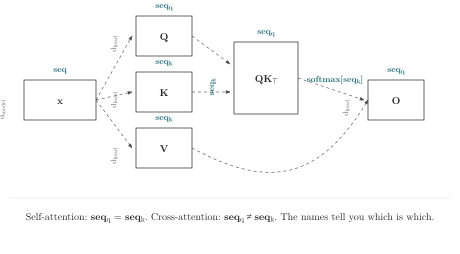
\includegraphics{figures/attention_flow.pdf}
\caption{Q, K, V coordinate flow: names distinguish self-attention from
cross-attention}
\end{figure}

The figure traces the coordinate flow through attention. On the left,
the input \(\mathbf{x}\) carries \texttt{seq} and \texttt{d\_model}.
Three projections branch off: \(\mathbf{Q}\) (with coordinate
\texttt{seq\_q} and \texttt{d\_head}), \(\mathbf{K}\) (with
\texttt{seq\_k} and \texttt{d\_head}), and \(\mathbf{V}\) (with
\texttt{seq\_k} and \texttt{d\_head}). The score matrix
\(\mathbf{QK}^\top\) sits in the center with axes \texttt{seq\_q} and
\texttt{seq\_k}---these are the two coordinates whose names encode the
architecture. After softmax over \texttt{seq\_k}, the output
\(\mathbf{O}\) carries \texttt{seq\_q} and \texttt{d\_head}. The bottom
panels spell out the distinction: in self-attention, \texttt{seq\_q} and
\texttt{seq\_k} range over the same sequence; in cross-attention,
\texttt{seq\_q} is the decoder positions and \texttt{seq\_k} is the
encoder positions. The coordinate names make the architecture decision
visible in the indices themselves.

\begin{Shaded}
\begin{Highlighting}[]
\CommentTok{// --- Multi-head self-attention ---}
\CommentTok{//}
\CommentTok{// Attention is a communication protocol with named roles:}
\CommentTok{//   seq_q = "who is asking" (the query position)}
\CommentTok{//   seq_k = "who is answering" (the key position)}
\CommentTok{//   head  = "which conversation" (isolated communication channel)}
\CommentTok{//   d_head = "the vocabulary" (what is being communicated)}
\CommentTok{//}
\CommentTok{// These four coordinates are not arbitrary. Each carries a distinct}
\CommentTok{// contract. seq_q and seq_k may be the same domain (self-attention) or}
\CommentTok{// different (cross-attention). head isolates gradient flow—heads do not}
\CommentTok{// compete. d_head is the inner dimension that gets contracted in the}
\CommentTok{// score computation. Every shape-compatible attention bug is a violation}
\CommentTok{// of one of these contracts.}
\KeywordTok{let}\NormalTok{ Q}\OperatorTok{[}\NormalTok{layer }\KeywordTok{in} \DecValTok{0.}\NormalTok{.n_layers, b, head, seq, d_head}\OperatorTok{]}\NormalTok{ =}
\NormalTok{    sum}\OperatorTok{[}\NormalTok{d_model}\OperatorTok{]}\NormalTok{(x}\OperatorTok{[}\NormalTok{layer, b, seq, d_model}\OperatorTok{]}\NormalTok{ *}
\NormalTok{                  Wq}\OperatorTok{[}\NormalTok{layer, head, d_model, d_head}\OperatorTok{]}\NormalTok{);}

\KeywordTok{let}\NormalTok{ K}\OperatorTok{[}\NormalTok{layer }\KeywordTok{in} \DecValTok{0.}\NormalTok{.n_layers, b, head, seq, d_head}\OperatorTok{]}\NormalTok{ =}
\NormalTok{    sum}\OperatorTok{[}\NormalTok{d_model}\OperatorTok{]}\NormalTok{(x}\OperatorTok{[}\NormalTok{layer, b, seq, d_model}\OperatorTok{]}\NormalTok{ *}
\NormalTok{                  Wk}\OperatorTok{[}\NormalTok{layer, head, d_model, d_head}\OperatorTok{]}\NormalTok{);}

\KeywordTok{let}\NormalTok{ V}\OperatorTok{[}\NormalTok{layer }\KeywordTok{in} \DecValTok{0.}\NormalTok{.n_layers, b, head, seq, d_head}\OperatorTok{]}\NormalTok{ =}
\NormalTok{    sum}\OperatorTok{[}\NormalTok{d_model}\OperatorTok{]}\NormalTok{(x}\OperatorTok{[}\NormalTok{layer, b, seq, d_model}\OperatorTok{]}\NormalTok{ *}
\NormalTok{                  Wv}\OperatorTok{[}\NormalTok{layer, head, d_model, d_head}\OperatorTok{]}\NormalTok{);}

\KeywordTok{let}\NormalTok{ scores}\OperatorTok{[}\NormalTok{layer }\KeywordTok{in} \DecValTok{0.}\NormalTok{.n_layers, b, head, seq_q, seq_k}\OperatorTok{]}\NormalTok{ =}
\NormalTok{    sum}\OperatorTok{[}\NormalTok{d_head}\OperatorTok{]}\NormalTok{(Q}\OperatorTok{[}\NormalTok{layer, b, head, seq_q, d_head}\OperatorTok{]}\NormalTok{ *}
\NormalTok{                 K}\OperatorTok{[}\NormalTok{layer, b, head, seq_k, d_head}\OperatorTok{]}\NormalTok{)}
\NormalTok{    / (d_head }\KeywordTok{as} \DataTypeTok{f32}\NormalTok{) ** }\DecValTok{0.5}\NormalTok{;}

\KeywordTok{let}\NormalTok{ masked_scores}\OperatorTok{[}\NormalTok{layer }\KeywordTok{in} \DecValTok{0.}\NormalTok{.n_layers, b, head, seq_q, seq_k}\OperatorTok{]}\NormalTok{ =}
    \KeywordTok{if}\NormalTok{ seq_k <= seq_q}
        \OperatorTok{\{}\NormalTok{ scores}\OperatorTok{[}\NormalTok{layer, b, head, seq_q, seq_k}\OperatorTok{]} \OperatorTok{\}}
        \KeywordTok{else} \OperatorTok{\{}\NormalTok{ -}\DecValTok{1}\NormalTok{e9 }\OperatorTok{\}}\NormalTok{;}

\KeywordTok{let}\NormalTok{ attn_weights}\OperatorTok{[}\NormalTok{layer }\KeywordTok{in} \DecValTok{0.}\NormalTok{.n_layers, b, head, seq_q, seq_k}\OperatorTok{]}\NormalTok{ =}
\NormalTok{    softmax}\OperatorTok{[}\NormalTok{seq_k}\OperatorTok{]}\NormalTok{(masked_scores}\OperatorTok{[}\NormalTok{layer, b, head, seq_q, seq_k}\OperatorTok{]}\NormalTok{);}

\KeywordTok{let}\NormalTok{ head_out}\OperatorTok{[}\NormalTok{layer }\KeywordTok{in} \DecValTok{0.}\NormalTok{.n_layers, b, head, seq_q, d_head}\OperatorTok{]}\NormalTok{ =}
\NormalTok{    sum}\OperatorTok{[}\NormalTok{seq_k}\OperatorTok{]}\NormalTok{(attn_weights}\OperatorTok{[}\NormalTok{layer, b, head, seq_q, seq_k}\OperatorTok{]}\NormalTok{ *}
\NormalTok{                V}\OperatorTok{[}\NormalTok{layer, b, head, seq_k, d_head}\OperatorTok{]}\NormalTok{);}

\KeywordTok{let}\NormalTok{ attn_out}\OperatorTok{[}\NormalTok{layer }\KeywordTok{in} \DecValTok{0.}\NormalTok{.n_layers, b, seq_q, d_model}\OperatorTok{]}\NormalTok{ =}
\NormalTok{    sum}\OperatorTok{[}\NormalTok{head, d_head}\OperatorTok{]}\NormalTok{(head_out}\OperatorTok{[}\NormalTok{layer, b, head, seq_q, d_head}\OperatorTok{]}\NormalTok{ *}
\NormalTok{                       Wo}\OperatorTok{[}\NormalTok{layer, head, d_head, d_model}\OperatorTok{]}\NormalTok{);}

\CommentTok{// --- Residual + LayerNorm ---}
\KeywordTok{let}\NormalTok{ x_post_attn}\OperatorTok{[}\NormalTok{layer }\KeywordTok{in} \DecValTok{0.}\NormalTok{.n_layers, b, seq, d_model}\OperatorTok{]}\NormalTok{ =}
\NormalTok{    x}\OperatorTok{[}\NormalTok{layer, b, seq, d_model}\OperatorTok{]}\NormalTok{ + attn_out}\OperatorTok{[}\NormalTok{layer, b, seq, d_model}\OperatorTok{]}\NormalTok{;}

\KeywordTok{let}\NormalTok{ mu}\OperatorTok{[}\NormalTok{layer }\KeywordTok{in} \DecValTok{0.}\NormalTok{.n_layers, b, seq}\OperatorTok{]}\NormalTok{ =}
\NormalTok{    mean}\OperatorTok{[}\NormalTok{d_model}\OperatorTok{]}\NormalTok{(x_post_attn}\OperatorTok{[}\NormalTok{layer, b, seq, d_model}\OperatorTok{]}\NormalTok{);}

\KeywordTok{let}\NormalTok{ sigma}\OperatorTok{[}\NormalTok{layer }\KeywordTok{in} \DecValTok{0.}\NormalTok{.n_layers, b, seq}\OperatorTok{]}\NormalTok{ =}
\NormalTok{    mean}\OperatorTok{[}\NormalTok{d_model}\OperatorTok{]}\NormalTok{((x_post_attn}\OperatorTok{[}\NormalTok{layer, b, seq, d_model}\OperatorTok{]}\NormalTok{ -}
\NormalTok{                    mu}\OperatorTok{[}\NormalTok{layer, b, seq}\OperatorTok{]}\NormalTok{) ** }\DecValTok{2.0}\NormalTok{) ** }\DecValTok{0.5}\NormalTok{;}

\KeywordTok{let}\NormalTok{ normed}\OperatorTok{[}\NormalTok{layer }\KeywordTok{in} \DecValTok{0.}\NormalTok{.n_layers, b, seq, d_model}\OperatorTok{]}\NormalTok{ =}
\NormalTok{    (x_post_attn}\OperatorTok{[}\NormalTok{layer, b, seq, d_model}\OperatorTok{]}\NormalTok{ - mu}\OperatorTok{[}\NormalTok{layer, b, seq}\OperatorTok{]}\NormalTok{)}
\NormalTok{    / (sigma}\OperatorTok{[}\NormalTok{layer, b, seq}\OperatorTok{]}\NormalTok{ + }\DecValTok{1}\NormalTok{e-}\DecValTok{5}\NormalTok{);}

\KeywordTok{let}\NormalTok{ ln_out}\OperatorTok{[}\NormalTok{layer }\KeywordTok{in} \DecValTok{0.}\NormalTok{.n_layers, b, seq, d_model}\OperatorTok{]}\NormalTok{ =}
\NormalTok{    normed}\OperatorTok{[}\NormalTok{layer, b, seq, d_model}\OperatorTok{]}\NormalTok{ * ln_scale}\OperatorTok{[}\NormalTok{layer, d_model}\OperatorTok{]}
\NormalTok{    + ln_bias}\OperatorTok{[}\NormalTok{layer, d_model}\OperatorTok{]}\NormalTok{;}

\CommentTok{// --- Feedforward ---}
\KeywordTok{let}\NormalTok{ ff_hidden}\OperatorTok{[}\NormalTok{layer }\KeywordTok{in} \DecValTok{0.}\NormalTok{.n_layers, b, seq, d_ff}\OperatorTok{]}\NormalTok{ =}
\NormalTok{    sum}\OperatorTok{[}\NormalTok{d_model}\OperatorTok{]}\NormalTok{(ln_out}\OperatorTok{[}\NormalTok{layer, b, seq, d_model}\OperatorTok{]}\NormalTok{ *}
\NormalTok{                  ff_w1}\OperatorTok{[}\NormalTok{layer, d_ff, d_model}\OperatorTok{]}\NormalTok{);}

\KeywordTok{let}\NormalTok{ ff_activated}\OperatorTok{[}\NormalTok{layer }\KeywordTok{in} \DecValTok{0.}\NormalTok{.n_layers, b, seq, d_ff}\OperatorTok{]}\NormalTok{ =}
    \KeywordTok{if}\NormalTok{ ff_hidden}\OperatorTok{[}\NormalTok{layer, b, seq, d_ff}\OperatorTok{]}\NormalTok{ > }\DecValTok{0.0}
        \OperatorTok{\{}\NormalTok{ ff_hidden}\OperatorTok{[}\NormalTok{layer, b, seq, d_ff}\OperatorTok{]} \OperatorTok{\}}
        \KeywordTok{else} \OperatorTok{\{} \DecValTok{0.0} \OperatorTok{\}}\NormalTok{;}

\KeywordTok{let}\NormalTok{ ff_out}\OperatorTok{[}\NormalTok{layer }\KeywordTok{in} \DecValTok{0.}\NormalTok{.n_layers, b, seq, d_model}\OperatorTok{]}\NormalTok{ =}
\NormalTok{    sum}\OperatorTok{[}\NormalTok{d_ff}\OperatorTok{]}\NormalTok{(ff_activated}\OperatorTok{[}\NormalTok{layer, b, seq, d_ff}\OperatorTok{]}\NormalTok{ *}
\NormalTok{               ff_w2}\OperatorTok{[}\NormalTok{layer, d_model, d_ff}\OperatorTok{]}\NormalTok{);}

\CommentTok{// --- Residual connection to next layer ---}
\KeywordTok{let}\NormalTok{ x}\OperatorTok{[}\NormalTok{layer+}\DecValTok{1}\NormalTok{, b, seq, d_model}\OperatorTok{]}\NormalTok{ =}
\NormalTok{    ln_out}\OperatorTok{[}\NormalTok{layer, b, seq, d_model}\OperatorTok{]}\NormalTok{ + ff_out}\OperatorTok{[}\NormalTok{layer, b, seq, d_model}\OperatorTok{]}\NormalTok{;}

\CommentTok{// === Output ===}
\KeywordTok{let}\NormalTok{ logits}\OperatorTok{[}\NormalTok{b, seq, vocab}\OperatorTok{]}\NormalTok{ =}
\NormalTok{    sum}\OperatorTok{[}\NormalTok{d_model}\OperatorTok{]}\NormalTok{(x}\OperatorTok{[}\NormalTok{n_layers, b, seq, d_model}\OperatorTok{]}\NormalTok{ * out_w}\OperatorTok{[}\NormalTok{vocab, d_model}\OperatorTok{]}\NormalTok{);}

\KeywordTok{let}\NormalTok{ probs}\OperatorTok{[}\NormalTok{b, seq, vocab}\OperatorTok{]}\NormalTok{ = softmax}\OperatorTok{[}\NormalTok{vocab}\OperatorTok{]}\NormalTok{(logits}\OperatorTok{[}\NormalTok{b, seq, vocab}\OperatorTok{]}\NormalTok{);}
\KeywordTok{let}\NormalTok{ loss = cross_entropy}\OperatorTok{[}\NormalTok{vocab}\OperatorTok{]}\NormalTok{(logits}\OperatorTok{[}\NormalTok{b, seq, vocab}\OperatorTok{]}\NormalTok{, labels}\OperatorTok{[}\NormalTok{b, seq}\OperatorTok{]}\NormalTok{);}

\CommentTok{// === Gradients ===}
\KeywordTok{let}\NormalTok{ dWq = @loss / @Wq;}
\KeywordTok{let}\NormalTok{ dWk = @loss / @Wk;}
\KeywordTok{let}\NormalTok{ dWv = @loss / @Wv;}
\KeywordTok{let}\NormalTok{ dWo = @loss / @Wo;}
\KeywordTok{let}\NormalTok{ d_ln_scale = @loss / @ln_scale;}
\KeywordTok{let}\NormalTok{ d_ln_bias = @loss / @ln_bias;}
\KeywordTok{let}\NormalTok{ d_ff_w1 = @loss / @ff_w1;}
\KeywordTok{let}\NormalTok{ d_ff_w2 = @loss / @ff_w2;}
\KeywordTok{let}\NormalTok{ d_out_w = @loss / @out_w;}
\end{Highlighting}
\end{Shaded}

``Looks clean,'' Jesse says. ``But we're going to read it with four
questions. Same four questions we'd ask of any tensor program. Ready?''

Dana nods. Jesse scrolls to the top.

\begin{center}\rule{0.5\linewidth}{0.4pt}\end{center}

\hypertarget{first-question-which-coordinate-is-being-eliminated}{%
\subsection{First Question: Which Coordinate Is Being
Eliminated?}\label{first-question-which-coordinate-is-being-eliminated}}

``The first thing I look at,'' Jesse says, ``is every reduction bracket.
What does the bracket claim to consume, and is that claim consistent
with the coordinates that survive?''

They scan the reductions together:

\begin{itemize}
\tightlist
\item
  \texttt{sum{[}d\_model{]}} in the Q, K, V projections. Consumes
  \texttt{d\_model}. Surviving:
  \texttt{{[}layer,\ b,\ head,\ seq,\ d\_head{]}}.
  Correct---\texttt{d\_model} is the inner dimension being contracted.
\item
  \texttt{sum{[}d\_head{]}} in the attention scores. Consumes
  \texttt{d\_head}. Surviving:
  \texttt{{[}layer,\ b,\ head,\ seq\_q,\ seq\_k{]}}. Correct.
\item
  \texttt{softmax{[}seq\_k{]}} in the attention weights. Consumes
  \texttt{seq\_k}. Surviving:
  \texttt{{[}layer,\ b,\ head,\ seq\_q,\ seq\_k{]}}. Wait.
\end{itemize}

``Softmax is a reduction,'' Jesse says. ``It consumes the coordinate in
its bracket---\texttt{seq\_k}---and reconstructs it with normalized
values. The coordinate \texttt{seq\_k} should survive with the same
domain. Does it?''

Dana checks the declaration. \texttt{attn\_weights} has coordinates
\texttt{{[}layer,\ b,\ head,\ seq\_q,\ seq\_k{]}}. Yes, \texttt{seq\_k}
survives. Good.

\begin{itemize}
\tightlist
\item
  \texttt{sum{[}seq\_k{]}} in the output computation. Consumes
  \texttt{seq\_k}. Surviving:
  \texttt{{[}layer,\ b,\ head,\ seq\_q,\ d\_head{]}}.
  Correct---\texttt{seq\_k} is the key dimension being weighted and
  summed.
\item
  \texttt{sum{[}head,\ d\_head{]}} in the output projection. Consumes
  both \texttt{head} and \texttt{d\_head}. Surviving:
  \texttt{{[}layer,\ b,\ seq\_q,\ d\_model{]}}. Correct---the heads are
  merged.
\end{itemize}

``The reductions are consistent,'' Jesse says. ``Every bracket names the
coordinate it consumes. No coordinate is consumed implicitly. Good.''

He scrolls down to the LayerNorm.

\begin{itemize}
\tightlist
\item
  \texttt{mean{[}d\_model{]}} for mu. Consumes \texttt{d\_model}.
  Surviving: \texttt{{[}layer,\ b,\ seq{]}}. Correct.
\item
  \texttt{mean{[}d\_model{]}} for sigma. Same.
\end{itemize}

``The reductions are clean. But there's a second question.''

\begin{center}\rule{0.5\linewidth}{0.4pt}\end{center}

\hypertarget{second-question-which-coordinate-is-being-copied-along}{%
\subsection{Second Question: Which Coordinate Is Being Copied
Along?}\label{second-question-which-coordinate-is-being-copied-along}}

Jesse points to the LayerNorm application:

\begin{Shaded}
\begin{Highlighting}[]
\KeywordTok{let}\NormalTok{ ln_out}\OperatorTok{[}\NormalTok{layer }\KeywordTok{in} \DecValTok{0.}\NormalTok{.n_layers, b, seq, d_model}\OperatorTok{]}\NormalTok{ =}
\NormalTok{    normed}\OperatorTok{[}\NormalTok{layer, b, seq, d_model}\OperatorTok{]}\NormalTok{ * ln_scale}\OperatorTok{[}\NormalTok{layer, d_model}\OperatorTok{]}
\NormalTok{    + ln_bias}\OperatorTok{[}\NormalTok{layer, d_model}\OperatorTok{]}\NormalTok{;}
\end{Highlighting}
\end{Shaded}

``\texttt{normed} has four coordinates:
\texttt{{[}layer,\ b,\ seq,\ d\_model{]}}. \texttt{ln\_scale} has two:
\texttt{{[}layer,\ d\_model{]}}. These are different ranks.''

Dana frowns. ``In einlang, broadcasting is only automatic for same-rank
tensors. A 4D tensor and a 2D tensor---the compiler won't broadcast
them. It requires explicit indexing when ranks differ.''

``So this line doesn't compile.''

Dana scrolls through the test logs. ``It compiled on the small-scale
test. But we were using a different broadcasting mode---the team added a
flag to allow cross-rank broadcasting during prototyping.''

``And that flag hides the fact that \texttt{b} and \texttt{seq} are
being silently replicated in the \texttt{ln\_scale} multiplication,''
Jesse says. ``The replication is mathematically correct---LayerNorm
\emph{should} be independent of batch and sequence position. But the
independence is invisible. A reader has to compare coordinate lists to
discover it.''

``The fix?'' Dana asks.

``You have two options. One: use a coordinate-aware function that makes
the independence part of its contract.''

\begin{Shaded}
\begin{Highlighting}[]
\KeywordTok{fn}\NormalTok{ layer_norm[feature](}
\NormalTok{    x: }\OperatorTok{[}\DataTypeTok{f32}\NormalTok{; ..batch, feature}\OperatorTok{]}\NormalTok{,}
\NormalTok{    scale: }\OperatorTok{[}\DataTypeTok{f32}\NormalTok{; feature}\OperatorTok{]}\NormalTok{,}
\NormalTok{    bias: }\OperatorTok{[}\DataTypeTok{f32}\NormalTok{; feature}\OperatorTok{]}
\NormalTok{) -> }\OperatorTok{[}\DataTypeTok{f32}\NormalTok{; ..batch, feature}\OperatorTok{]} \OperatorTok{\{}
    \KeywordTok{let}\NormalTok{ mu}\OperatorTok{[}\NormalTok{..batch}\OperatorTok{]}\NormalTok{ = mean}\OperatorTok{[}\NormalTok{feature}\OperatorTok{]}\NormalTok{(x}\OperatorTok{[}\NormalTok{..batch, feature}\OperatorTok{]}\NormalTok{);}
    \KeywordTok{let}\NormalTok{ sigma}\OperatorTok{[}\NormalTok{..batch}\OperatorTok{]}\NormalTok{ = mean}\OperatorTok{[}\NormalTok{feature}\OperatorTok{]}\NormalTok{((x}\OperatorTok{[}\NormalTok{..batch, feature}\OperatorTok{]}\NormalTok{ - mu}\OperatorTok{[}\NormalTok{..batch}\OperatorTok{]}\NormalTok{) ** }\DecValTok{2.0}\NormalTok{) ** }\DecValTok{0.5}\NormalTok{;}
    \KeywordTok{let}\NormalTok{ normed}\OperatorTok{[}\NormalTok{..batch, feature}\OperatorTok{]}\NormalTok{ = (x}\OperatorTok{[}\NormalTok{..batch, feature}\OperatorTok{]}\NormalTok{ - mu}\OperatorTok{[}\NormalTok{..batch}\OperatorTok{]}\NormalTok{) / (sigma}\OperatorTok{[}\NormalTok{..batch}\OperatorTok{]}\NormalTok{ + }\DecValTok{1}\NormalTok{e-}\DecValTok{5}\NormalTok{);}
\NormalTok{    normed}\OperatorTok{[}\NormalTok{..batch, feature}\OperatorTok{]}\NormalTok{ * scale}\OperatorTok{[}\NormalTok{feature}\OperatorTok{]}\NormalTok{ + bias}\OperatorTok{[}\NormalTok{feature}\OperatorTok{]}
\OperatorTok{\}}
\end{Highlighting}
\end{Shaded}

``Now the fact that \texttt{scale} and \texttt{bias} are independent of
everything except \texttt{feature} is visible in their type signatures.
The rest packs \texttt{..batch} absorb whatever leading coordinates the
caller provides. No implicit broadcasting. No cross-rank surprises.''

``Option two,'' Dana says, ``is to make the broadcasting explicit inline
by indexing \texttt{ln\_scale} at the full coordinate set and letting
the compiler verify the omission:''

\begin{Shaded}
\begin{Highlighting}[]
\CommentTok{// Explicit: ln_scale omits b and seq by not mentioning them}
\KeywordTok{let}\NormalTok{ ln_out}\OperatorTok{[}\NormalTok{layer, b, seq, d_model}\OperatorTok{]}\NormalTok{ =}
\NormalTok{    normed}\OperatorTok{[}\NormalTok{layer, b, seq, d_model}\OperatorTok{]}\NormalTok{ * ln_scale}\OperatorTok{[}\NormalTok{layer, d_model}\OperatorTok{]}
\NormalTok{    + ln_bias}\OperatorTok{[}\NormalTok{layer, d_model}\OperatorTok{]}\NormalTok{;}
\end{Highlighting}
\end{Shaded}

``But this still relies on implicit broadcasting for different ranks,''
Jesse says. ``The function approach is safer. Either way, the point is:
the independence of the normalization parameters from the batch
dimensions should be a visible fact in the code, not a consequence of
the broadcasting engine's behavior.''

Dana makes a note. ``Use the function. It's one more abstraction, but
the contract is checkable.''

\begin{center}\rule{0.5\linewidth}{0.4pt}\end{center}

\hypertarget{third-question-can-you-trace-a-coordinate-from-source-to-destination}{%
\subsection{Third Question: Can You Trace a Coordinate from Source to
Destination?}\label{third-question-can-you-trace-a-coordinate-from-source-to-destination}}

Jesse scrolls to the attention output and the residual connection.

\begin{Shaded}
\begin{Highlighting}[]
\KeywordTok{let}\NormalTok{ attn_out}\OperatorTok{[}\NormalTok{layer }\KeywordTok{in} \DecValTok{0.}\NormalTok{.n_layers, b, seq_q, d_model}\OperatorTok{]}\NormalTok{ =}
\NormalTok{    sum}\OperatorTok{[}\NormalTok{head, d_head}\OperatorTok{]}\NormalTok{(head_out}\OperatorTok{[}\NormalTok{layer, b, head, seq_q, d_head}\OperatorTok{]}\NormalTok{ *}
\NormalTok{                       Wo}\OperatorTok{[}\NormalTok{layer, head, d_head, d_model}\OperatorTok{]}\NormalTok{);}

\KeywordTok{let}\NormalTok{ x_post_attn}\OperatorTok{[}\NormalTok{layer }\KeywordTok{in} \DecValTok{0.}\NormalTok{.n_layers, b, seq, d_model}\OperatorTok{]}\NormalTok{ =}
\NormalTok{    x}\OperatorTok{[}\NormalTok{layer, b, seq, d_model}\OperatorTok{]}\NormalTok{ + attn_out}\OperatorTok{[}\NormalTok{layer, b, seq, d_model}\OperatorTok{]}\NormalTok{;}
\end{Highlighting}
\end{Shaded}

``Look at the coordinate names,'' Jesse says. ``The attention output
declares its sequence coordinate as \texttt{seq\_q}. The residual
connection indexes it as \texttt{seq}. Are these the same coordinate?''

Dana studies the two lines. ``In self-attention, they're the same
domain. The query sequence and the key sequence are the same tokens. So
\texttt{seq\_q} and \texttt{seq} refer to the same thing.''

``Then why do they have different names?''

Dana is quiet for a moment. ``Because I wrote the attention block first,
using \texttt{seq\_q} and \texttt{seq\_k} to make the roles clear inside
the attention computation. Then I wrote the residual connection and used
\texttt{seq} because the role distinction wasn't needed outside
attention.''

``So the same domain has two names. The compiler sees \texttt{seq\_q}
and \texttt{seq} as different coordinates. If they have the same extent,
the residual addition might compile---einlang allows addition of tensors
with different coordinate names if the extents match and the compiler
can verify the correspondence. But there's a flag for that too. If the
extents differ---say, in a cross-attention scenario where the query
length and key length are different---this residual connection would
produce a shape mismatch.''

``Or worse,'' Dana says, ``if the extents happen to be equal but the
domains are actually different, the addition would silently produce a
valid tensor with semantically wrong values. The Square Matrix Test.''

``Exactly. The fix is simple: use \texttt{seq} consistently for
self-attention. If you need \texttt{seq\_q} and \texttt{seq\_k} inside
the attention computation for clarity, rename at the boundary.''

Dana rewrites:

\begin{Shaded}
\begin{Highlighting}[]
\KeywordTok{let}\NormalTok{ attn_out}\OperatorTok{[}\NormalTok{layer }\KeywordTok{in} \DecValTok{0.}\NormalTok{.n_layers, b, seq, d_model}\OperatorTok{]}\NormalTok{ =}
\NormalTok{    sum}\OperatorTok{[}\NormalTok{head, d_head}\OperatorTok{]}\NormalTok{(head_out}\OperatorTok{[}\NormalTok{layer, b, head, seq, d_head}\OperatorTok{]}\NormalTok{ *}
\NormalTok{                       Wo}\OperatorTok{[}\NormalTok{layer, head, d_head, d_model}\OperatorTok{]}\NormalTok{);}
\end{Highlighting}
\end{Shaded}

``Now \texttt{seq} flows from the input embedding, through every layer,
to the output projection. One name, one identity, traceable from source
to destination.''

``That's the third habit,'' Jesse says. ``Permute with a source. But it
applies even when there's no permutation---just a coordinate renaming.
If a coordinate has the same identity throughout the computation, use
the same name. If it doesn't, the place where the name changes is the
place where the identity changes. That place should be visible.''

\begin{center}\rule{0.5\linewidth}{0.4pt}\end{center}

\hypertarget{fourth-question-the-declaration-bracket}{%
\subsection{Fourth Question: The Declaration
Bracket}\label{fourth-question-the-declaration-bracket}}

Jesse points to the recurrence that connects layers:

\begin{Shaded}
\begin{Highlighting}[]
\KeywordTok{let}\NormalTok{ x}\OperatorTok{[}\NormalTok{layer+}\DecValTok{1}\NormalTok{, b, seq, d_model}\OperatorTok{]}\NormalTok{ =}
\NormalTok{    ln_out}\OperatorTok{[}\NormalTok{layer, b, seq, d_model}\OperatorTok{]}\NormalTok{ + ff_out}\OperatorTok{[}\NormalTok{layer, b, seq, d_model}\OperatorTok{]}\NormalTok{;}
\end{Highlighting}
\end{Shaded}

``Read the declaration bracket.''

Dana reads: \texttt{x{[}layer+1,\ ...{]}}. She closes her eyes. ``Ah.''

``The declaration bracket can only contain identifiers, literals, and
named rests. No expressions. \texttt{layer+1} is an expression.''

``I put the computation in the wrong place,'' Dana says. ``The bracket
is for naming \emph{what} is being defined---the element at index
\texttt{layer+1} over some domain. The body is for saying \emph{how} to
compute it, using backward references like \texttt{layer-1}.''

She rewrites:

\begin{Shaded}
\begin{Highlighting}[]
\KeywordTok{let}\NormalTok{ x}\OperatorTok{[}\NormalTok{layer }\KeywordTok{in} \DecValTok{1.}\NormalTok{.=n_layers, b, seq, d_model}\OperatorTok{]}\NormalTok{ =}
\NormalTok{    ln_out}\OperatorTok{[}\NormalTok{layer-}\DecValTok{1}\NormalTok{, b, seq, d_model}\OperatorTok{]}\NormalTok{ + ff_out}\OperatorTok{[}\NormalTok{layer-}\DecValTok{1}\NormalTok{, b, seq, d_model}\OperatorTok{]}\NormalTok{;}
\end{Highlighting}
\end{Shaded}

``Now the declaration bracket says \texttt{layer\ in\ 1..=n\_layers}---a
domain, not an expression. The body uses \texttt{layer-1}---a backward
reference, which is allowed because \texttt{layer-1} is strictly smaller
than \texttt{layer}. The rule is consistent: the left side names the
element being defined. The right side computes it from earlier
elements.''

``This is the same rule from Chapter 3,'' Jesse says. ``The index slot
in the declaration bracket is for naming, not computing. It's not an
arbitrary syntactic restriction. It's what makes the backward-only
constraint checkable. If \texttt{layer+1} were allowed in the bracket,
the compiler couldn't statically verify that the recurrence only reads
from the past.''

\begin{center}\rule{0.5\linewidth}{0.4pt}\end{center}

\hypertarget{the-gradient-question}{%
\subsection{The Gradient Question}\label{the-gradient-question}}

Jesse scrolls to the bottom.

\begin{Shaded}
\begin{Highlighting}[]
\KeywordTok{let}\NormalTok{ dWq = @loss / @Wq;}
\KeywordTok{let}\NormalTok{ dWk = @loss / @Wk;}
\KeywordTok{let}\NormalTok{ dWv = @loss / @Wv;}
\KeywordTok{let}\NormalTok{ dWo = @loss / @Wo;}
\KeywordTok{let}\NormalTok{ d_out_w = @loss / @out_w;}
\end{Highlighting}
\end{Shaded}

``What are the coordinates of \texttt{d\_out\_w}?''

Dana thinks. ``\texttt{out\_w} has coordinates
\texttt{{[}vocab,\ d\_model{]}}. The forward pass uses it in
\texttt{sum{[}d\_model{]}(x{[}...{]}\ *\ out\_w{[}vocab,\ d\_model{]})}.
The gradient with respect to \texttt{out\_w} must sum over all
coordinates that \texttt{out\_w} omits---which are \texttt{b} and
\texttt{seq}. So \texttt{d\_out\_w} should have coordinates
\texttt{{[}vocab,\ d\_model{]}}.''

``And if the compiler accidentally summed over \texttt{vocab} instead,
producing \texttt{{[}b,\ seq,\ d\_model{]}}?''

``Then the gradient would have the wrong shape. Except---if
\texttt{vocab} happened to equal \texttt{d\_model}---''

``Square Matrix Test again. The shapes would match by coincidence. The
optimizer would apply an invalid gradient update. The loss would still
go down---just for the wrong reasons.''

Dana is silent for a moment. ``How do we verify this?''

``You don't need to. The compiler does. The autodiff rules from Chapter
8 guarantee that \texttt{@loss\ /\ @out\_w} sums over exactly the
coordinates that \texttt{out\_w} omits. The coordinate structure of the
gradient is determined by the coordinate structure of the forward pass.
But the question---`does the backward reduction match the forward
omission?'---is exactly the fourth habit. Forward and backward,
symmetric. You ask it to verify that you trust the compiler's answer.''

\begin{center}\rule{0.5\linewidth}{0.4pt}\end{center}

\hypertarget{the-conversation-continues-cross-attention}{%
\subsection{The Conversation Continues:
Cross-Attention}\label{the-conversation-continues-cross-attention}}

Jesse leans back. ``The code is correct for self-attention. But the
architecture document mentions cross-attention for the second
phase---the decoder attending to the encoder output. How would you
extend this?''

Dana opens a fresh buffer. ``Cross-attention means the queries come from
one sequence and the keys and values come from another. The two
sequences may have different lengths and different coordinate
identities.''

She sketches:

\begin{Shaded}
\begin{Highlighting}[]
\CommentTok{// Encoder output: sequence of source tokens}
\KeywordTok{let}\NormalTok{ enc_out}\OperatorTok{[}\NormalTok{enc_seq, d_model}\OperatorTok{]}\NormalTok{ = encoder(source);}

\CommentTok{// Decoder hidden state: sequence of target tokens (so far)}
\KeywordTok{let}\NormalTok{ dec_hidden}\OperatorTok{[}\NormalTok{dec_seq, d_model}\OperatorTok{]}\NormalTok{ = decoder_embedding(target_prefix);}

\CommentTok{// Cross-attention: decoder queries attend to encoder keys/values}
\KeywordTok{let}\NormalTok{ Q_cross}\OperatorTok{[}\NormalTok{b, head, dec_seq, d_head}\OperatorTok{]}\NormalTok{ =}
\NormalTok{    sum}\OperatorTok{[}\NormalTok{d_model}\OperatorTok{]}\NormalTok{(dec_hidden}\OperatorTok{[}\NormalTok{dec_seq, d_model}\OperatorTok{]}\NormalTok{ *}
\NormalTok{                  Wq_cross}\OperatorTok{[}\NormalTok{head, d_model, d_head}\OperatorTok{]}\NormalTok{);}

\KeywordTok{let}\NormalTok{ K_cross}\OperatorTok{[}\NormalTok{b, head, enc_seq, d_head}\OperatorTok{]}\NormalTok{ =}
\NormalTok{    sum}\OperatorTok{[}\NormalTok{d_model}\OperatorTok{]}\NormalTok{(enc_out}\OperatorTok{[}\NormalTok{enc_seq, d_model}\OperatorTok{]}\NormalTok{ *}
\NormalTok{                  Wk_cross}\OperatorTok{[}\NormalTok{head, d_model, d_head}\OperatorTok{]}\NormalTok{);}

\KeywordTok{let}\NormalTok{ V_cross}\OperatorTok{[}\NormalTok{b, head, enc_seq, d_head}\OperatorTok{]}\NormalTok{ =}
\NormalTok{    sum}\OperatorTok{[}\NormalTok{d_model}\OperatorTok{]}\NormalTok{(enc_out}\OperatorTok{[}\NormalTok{enc_seq, d_model}\OperatorTok{]}\NormalTok{ *}
\NormalTok{                  Wv_cross}\OperatorTok{[}\NormalTok{head, d_model, d_head}\OperatorTok{]}\NormalTok{);}

\KeywordTok{let}\NormalTok{ scores_cross}\OperatorTok{[}\NormalTok{b, head, dec_seq, enc_seq}\OperatorTok{]}\NormalTok{ =}
\NormalTok{    sum}\OperatorTok{[}\NormalTok{d_head}\OperatorTok{]}\NormalTok{(Q_cross}\OperatorTok{[}\NormalTok{b, head, dec_seq, d_head}\OperatorTok{]}\NormalTok{ *}
\NormalTok{                 K_cross}\OperatorTok{[}\NormalTok{b, head, enc_seq, d_head}\OperatorTok{]}\NormalTok{)}
\NormalTok{    / (d_head }\KeywordTok{as} \DataTypeTok{f32}\NormalTok{) ** }\DecValTok{0.5}\NormalTok{;}

\KeywordTok{let}\NormalTok{ attn_cross}\OperatorTok{[}\NormalTok{b, head, dec_seq, enc_seq}\OperatorTok{]}\NormalTok{ =}
\NormalTok{    softmax}\OperatorTok{[}\NormalTok{enc_seq}\OperatorTok{]}\NormalTok{(scores_cross}\OperatorTok{[}\NormalTok{b, head, dec_seq, enc_seq}\OperatorTok{]}\NormalTok{);}

\KeywordTok{let}\NormalTok{ cross_out}\OperatorTok{[}\NormalTok{b, head, dec_seq, d_head}\OperatorTok{]}\NormalTok{ =}
\NormalTok{    sum}\OperatorTok{[}\NormalTok{enc_seq}\OperatorTok{]}\NormalTok{(attn_cross}\OperatorTok{[}\NormalTok{b, head, dec_seq, enc_seq}\OperatorTok{]}\NormalTok{ *}
\NormalTok{                  V_cross}\OperatorTok{[}\NormalTok{b, head, enc_seq, d_head}\OperatorTok{]}\NormalTok{);}
\end{Highlighting}
\end{Shaded}

Jesse studies the coordinate names. ``\texttt{dec\_seq} and
\texttt{enc\_seq} are different. The score matrix is
\texttt{{[}...,\ dec\_seq,\ enc\_seq{]}}---query positions on one axis,
key positions on the other. If someone accidentally used \texttt{seq}
for both, the compiler would see a square matrix and the attention would
silently become self-attention.''

``If the lengths are different, the shape mismatch would catch it,''
Dana says. ``But if the lengths happen to be equal---the Square Matrix
Test, again---the bug survives. Distinct names make it survive the
compiler instead.''

``This is exactly why the attention block in the original code used
\texttt{seq\_q} and \texttt{seq\_k}---the convention anticipates
cross-attention. In self-attention, both happen to be \texttt{seq}. In
cross-attention, one is \texttt{dec\_seq} and the other is
\texttt{enc\_seq}. The naming convention makes the architecture visible
in the coordinate names.''

Dana nods. ``And the compiler enforces it. If I try to compute
\texttt{scores\_cross} with \texttt{Q{[}dec\_seq{]}} and
\texttt{K{[}enc\_seq{]}} but label the result \texttt{{[}seq,\ seq{]}},
the compiler will report that \texttt{dec\_seq} and \texttt{enc\_seq}
don't match the declared coordinate. The names are part of the type.''

\begin{center}\rule{0.5\linewidth}{0.4pt}\end{center}

\hypertarget{the-conversation-deepens-multi-query-attention}{%
\subsection{The Conversation Deepens: Multi-Query
Attention}\label{the-conversation-deepens-multi-query-attention}}

``While we're on attention variants,'' Jesse says, ``the team has been
talking about multi-query attention for the next iteration. Fewer
key-value heads than query heads, to reduce the KV cache size. How does
that change the coordinate structure?''

Dana thinks for a moment. ``In multi-head attention, every query head
has its own key head and value head. The coordinate \texttt{head} spans
query, key, and value equally. In multi-query attention, the query has
\texttt{n\_heads} heads but the keys and values share a single head---or
a smaller number of heads.''

``So the \texttt{head} coordinate has different extents for Q vs.~K/V.''

``Exactly. And if you use the same coordinate name \texttt{head} for
both, you're claiming they're the same domain---which they aren't, or
aren't entirely. The notation should make that visible.''

She sketches the multi-query variant:

\begin{Shaded}
\begin{Highlighting}[]
\CommentTok{// Multi-query attention: many query heads, fewer key-value heads}
\KeywordTok{let}\NormalTok{ n_q_heads = }\DecValTok{8}\NormalTok{;}
\KeywordTok{let}\NormalTok{ n_kv_heads = }\DecValTok{2}\NormalTok{;   }\CommentTok{// shared across query heads}

\KeywordTok{let}\NormalTok{ Wq}\OperatorTok{[}\NormalTok{head_q, d_model, d_head}\OperatorTok{]}\NormalTok{ = init_weight(n_q_heads, d_model, d_head);}
\KeywordTok{let}\NormalTok{ Wk}\OperatorTok{[}\NormalTok{head_kv, d_model, d_head}\OperatorTok{]}\NormalTok{ = init_weight(n_kv_heads, d_model, d_head);}
\KeywordTok{let}\NormalTok{ Wv}\OperatorTok{[}\NormalTok{head_kv, d_model, d_head}\OperatorTok{]}\NormalTok{ = init_weight(n_kv_heads, d_model, d_head);}

\KeywordTok{let}\NormalTok{ Q}\OperatorTok{[}\NormalTok{b, head_q, seq, d_head}\OperatorTok{]}\NormalTok{ = sum}\OperatorTok{[}\NormalTok{d_model}\OperatorTok{]}\NormalTok{(x}\OperatorTok{[}\NormalTok{b, seq, d_model}\OperatorTok{]}\NormalTok{ * Wq}\OperatorTok{[}\NormalTok{head_q, d_model, d_head}\OperatorTok{]}\NormalTok{);}
\KeywordTok{let}\NormalTok{ K}\OperatorTok{[}\NormalTok{b, head_kv, seq, d_head}\OperatorTok{]}\NormalTok{ = sum}\OperatorTok{[}\NormalTok{d_model}\OperatorTok{]}\NormalTok{(x}\OperatorTok{[}\NormalTok{b, seq, d_model}\OperatorTok{]}\NormalTok{ * Wk}\OperatorTok{[}\NormalTok{head_kv, d_model, d_head}\OperatorTok{]}\NormalTok{);}
\KeywordTok{let}\NormalTok{ V}\OperatorTok{[}\NormalTok{b, head_kv, seq, d_head}\OperatorTok{]}\NormalTok{ = sum}\OperatorTok{[}\NormalTok{d_model}\OperatorTok{]}\NormalTok{(x}\OperatorTok{[}\NormalTok{b, seq, d_model}\OperatorTok{]}\NormalTok{ * Wv}\OperatorTok{[}\NormalTok{head_kv, d_model, d_head}\OperatorTok{]}\NormalTok{);}

\CommentTok{// The score: for each head_q, use the corresponding head_kv group}
\KeywordTok{let}\NormalTok{ scores}\OperatorTok{[}\NormalTok{b, head_q, seq_q, seq_k}\OperatorTok{]}\NormalTok{ =}
\NormalTok{    sum}\OperatorTok{[}\NormalTok{d_head}\OperatorTok{]}\NormalTok{(Q}\OperatorTok{[}\NormalTok{b, head_q, seq_q, d_head}\OperatorTok{]}\NormalTok{ *}
\NormalTok{                 K}\OperatorTok{[}\NormalTok{b, head_kv_of}\OperatorTok{[}\NormalTok{head_q}\OperatorTok{]}\NormalTok{, seq_k, d_head}\OperatorTok{]}\NormalTok{)}
\NormalTok{    / (d_head }\KeywordTok{as} \DataTypeTok{f32}\NormalTok{) ** }\DecValTok{0.5}\NormalTok{;}
\end{Highlighting}
\end{Shaded}

Jesse points at the last line.
``\texttt{head\_kv\_of{[}head\_q{]}}---what's that?''

``A mapping from query heads to key-value heads. If
\texttt{n\_q\_heads\ =\ 8} and \texttt{n\_kv\_heads\ =\ 2}, then
\texttt{head\_kv\_of} maps query heads 0-3 to KV head 0, and query heads
4-7 to KV head 1. It's an explicit function, not an implicit broadcast.
The coordinate names---\texttt{head\_q} vs. \texttt{head\_kv}---make the
structural asymmetry visible. You can't accidentally treat them as the
same coordinate because they have different names.''

``And the shapes?''

``Q has \texttt{{[}b,\ head\_q,\ seq,\ d\_head{]}}. K has
\texttt{{[}b,\ head\_kv,\ seq,\ d\_head{]}}. The score computation needs
to align \texttt{head\_q} with \texttt{head\_kv} via the mapping. A
standard \texttt{sum{[}d\_head{]}} won't work because the \texttt{head}
coordinates don't match. The compiler would reject a naive contraction
attempt. The mapping \texttt{head\_kv\_of{[}head\_q{]}} is
required---and checked.''

``This is the coordinate habit applied to architecture design,'' Jesse
says. ``The notation doesn't just record the architecture. It constrains
it. A shape-compatible bug---using the wrong KV head for a query
head---is a coordinate mismatch. The compiler catches it.''

\begin{center}\rule{0.5\linewidth}{0.4pt}\end{center}

\hypertarget{what-survives-the-audit}{%
\subsection{What Survives the Audit}\label{what-survives-the-audit}}

Dana commits the changes:

\begin{enumerate}
\def\labelenumi{\arabic{enumi}.}
\item
  \textbf{LayerNorm} is wrapped in a coordinate-aware function with rest
  packs. The independence of scale and bias from batch coordinates is
  visible in the type signature.
\item
  \textbf{The \texttt{seq\_q} coordinate} in \texttt{attn\_out} is
  renamed to \texttt{seq}. One name, one identity, from embedding to
  output.
\item
  \textbf{The recurrence} uses \texttt{layer\ in\ 1..=n\_layers} in the
  declaration bracket and \texttt{layer-1} in the body. The left side
  names. The right side computes.
\item
  \textbf{The gradient coordinates} are verified: each
  \texttt{@loss\ /\ @param} has the same coordinates as \texttt{param}.
  The compiler enforces this. The audit confirms it.
\item
  \textbf{Cross-attention} uses distinct coordinate names for decoder
  sequence (\texttt{dec\_seq}) and encoder sequence (\texttt{enc\_seq}).
  The architecture is visible in the names.
\item
  \textbf{Multi-query attention} uses distinct coordinate names for
  query heads (\texttt{head\_q}) and key-value heads
  (\texttt{head\_kv}), with an explicit mapping between them. The
  structural asymmetry is a coordinate-level fact.
\end{enumerate}

It is 11:14 PM. The GPUs are still reserved for 8 AM. The code is
different than it was two hours ago---not in what it computes, but in
what it says. The shapes are the same. The names are clearer. The
compiler has more to check, and the next reader---Dana, three months
from now, after the model architecture has changed twice---has more to
read.

``That's the whole thing, isn't it?'' Dana says. ``The coordinate habit
isn't about writing correct code. It's about writing code that stays
correct when you're not the one reading it.''

Jesse closes the laptop. ``See you Saturday.''

\begin{center}\rule{0.5\linewidth}{0.4pt}\end{center}

This is the graduation. You can now read a tensor program and see not
just the shapes, but the coordinates---which survive, which are
consumed, which are broadcast, which are reduced. The four habits are
not something you apply deliberately, one at a time, with effort. They
are how you read.

Every reduction bracket is a claim about which coordinate is eliminated.
Every broadcast is a claim about which coordinate is independent. Every
coordinate name is a claim about identity---where the data came from,
where it is going, whether the name at the destination matches the name
at the source. The gradient of a loss with respect to a parameter is a
claim about which coordinates the parameter omitted in the forward pass.

The compiler checks these claims. The habits check the compiler. And the
notation makes both possible.

\hypertarget{try-it-15}{%
\subsubsection{Try It}\label{try-it-15}}

\begin{enumerate}
\def\labelenumi{\arabic{enumi}.}
\item
  In the cross-attention sketch, the softmax is over \texttt{enc\_seq}.
  What would happen if someone changed it to
  \texttt{softmax{[}dec\_seq{]}}? The shapes would be identical---a
  probability distribution over the decoder positions instead of the
  encoder positions. How would you catch this in code review?
\item
  Multi-query attention with \texttt{head\_kv\_of{[}head\_q{]}} requires
  a mapping function. If \texttt{n\_q\_heads\ =\ 8} and
  \texttt{n\_kv\_heads\ =\ 4}, and query heads 0-1 map to KV head 0,
  heads 2-3 to KV head 1, etc., write the mapping as an einlang
  expression. What would the compiler check?
\item
  \textbf{Mixture of Experts.} A routing operation
  \texttt{let\ route{[}b,\ t{]}\ =\ argmax{[}e{]}(gate\_prob{[}b,\ t,\ e{]});}
  sends each token to its top expert. Each expert has a capacity limit.
  Tokens beyond capacity are silently dropped---their output is replaced
  by a fallback value. The mask \texttt{keep{[}b,\ t{]}} records which
  tokens survived. This mask has the same shape as the output; it does
  not change any dimension. The fact that some tokens were silently
  replaced is invisible to every shape check. How would you make this
  fact visible in the notation? Think about what coordinate you would
  name, and what the mask's presence or absence in the coordinate list
  tells the reader.
\end{enumerate}

\newpage

\hypertarget{epilogue-a-friend-named-einlang}{%
\section{Epilogue · A Friend Named
einlang}\label{epilogue-a-friend-named-einlang}}

\begin{quote}
``Programs must be written for people to read, and only incidentally for
machines to execute.''

--- Harold Abelson and Gerald Jay Sussman, \emph{Structure and
Interpretation of Computer Programs}
\end{quote}

\begin{center}\rule{0.5\linewidth}{0.4pt}\end{center}

In Chapter 6, einlang was a name. A label for the notation we'd been
building since Chapter 3. Now, at the end of sixteen chapters, you know
what the name actually refers to.

Einlang is not a language in the sense that Python is a language, or
C++, or Rust. It does not aspire to run your web server or render your
UI. It is a language built on three ideas: primitive expressions, means
of combination, and means of abstraction---organized around a single
purpose.

The idea is that \textbf{coordinates have identities, and those
identities belong in the source code.}

Everything else in the language serves that idea. Reductions name the
coordinate they consume. Broadcasts name the coordinate they replicate
along. Permutations state the coordinate correspondence explicitly.
Functions declare which coordinates they use by identity, and the
compiler checks those declarations at every call site. Gradients
preserve coordinate structure through differentiation. Recurrences make
the direction of time a syntactic constraint.

\begin{center}\rule{0.5\linewidth}{0.4pt}\end{center}

The SICP quotation that opens this epilogue is famous for a reason. It
states a truth that is obvious once you hear it and difficult to
practice consistently: code is communication between humans before it is
instruction to machines.

The coordinate habit is an application of that truth to tensor
programming. When you write \texttt{x.mean(dim=1)}, you are
communicating to the machine (``reduce axis 1'') but not to the human
(``eliminate channel''). When you write \texttt{mean{[}channel{]}(x)},
you are communicating to both. The machine still knows what to do. The
human now also knows what you intended. And the compiler can check that
your intent is consistent with the tensor's actual coordinate structure.

This is the bet the book has asked you to make: that the extra
keystrokes of naming coordinates are repaid, with interest, in debugging
sessions avoided, in refactoring confidence gained, in the quiet
satisfaction of reading code that says what it means.

\begin{center}\rule{0.5\linewidth}{0.4pt}\end{center}

SICP ends with a meta-circular evaluator---a Scheme interpreter written
in Scheme---as if to say: you now understand the language deeply enough
to implement it yourself.

I am not going to ask you to implement einlang. I am going to ask you
something smaller and harder.

Take the four habits into your next tensor program. Not an einlang
program---the language is young, the tooling is sparse, and you have
deadlines. Take them into PyTorch. Into JAX. Into whatever framework you
use to get work done.

When you write a reduction, pause. Ask: which coordinate am I
eliminating? Is the name in the code?

When you write a broadcast, pause. Ask: which coordinate am I copying
along? Is independence genuinely justified?

When you write a permutation, pause. Ask: can I trace one coordinate
from source to destination without reconstructing the position map?

When you inspect a gradient, pause. Ask: does the backward reduction
match the forward broadcast?

These questions cost seconds. The bugs they catch cost hours. The ratio
is favorable.

\begin{center}\rule{0.5\linewidth}{0.4pt}\end{center}

\hypertarget{how-to-start}{%
\subsection{How to Start}\label{how-to-start}}

You don't need einlang to practice the coordinate habit. You need a
place to put a name and a discipline to keep it honest.

Start small. Name one coordinate at a time. The data-entry boundary is
the most important one---if coordinates are named when tensors enter the
program, the names flow downstream. Name the reductions next---they are
where coordinates are consumed, and the consumption is the hardest fact
to reconstruct later. Name the broadcasts last---they are often
implicit, and making them explicit is the most verbose change.

In PyTorch, a comment is your first bridge:
\texttt{x.mean(dim=1)\ \ \#\ dim\ 1\ =\ channel}. In JAX, einops
patterns are your bridge:
\texttt{rearrange(x,\ "batch\ channel\ spatial\ -\textgreater{}\ batch\ spatial\ channel")}.
The bridge doesn't have to be perfect. It has to be there.

The goal is not to convert your entire codebase to named dimensions
overnight. The goal is to develop the reflex: when you write an
operation that depends on a coordinate's identity, put that identity in
the source. Not in your head. Not in a Slack message. In the source.

\begin{center}\rule{0.5\linewidth}{0.4pt}\end{center}

There is a sentence I have been saving for the end. It is the
one-sentence version of this book:

\textbf{Let your coordinate names be as visible as your intent---because
six months from now, when you return to this code to fix a bug, the
intent will be gone, and only the names will remain.}

Thank you for reading.

\newpage

\end{document}
